% !TEX program = xelatex
\documentclass[UTF8,a4paper,12pt]{ctexart}
\usepackage{geometry}
\geometry{left=2.6cm,right=2.6cm,top=2.7cm,bottom=2.6cm}
\usepackage{amsmath,amssymb,bm}
\usepackage{graphicx}
\usepackage{booktabs,array,multirow}
% 子图改用 minipage 实现，无需 subcaption 宏包
\usepackage{enumitem}
\usepackage{float}
\usepackage{xcolor}
\usepackage{fancyhdr}
\usepackage{setspace}
\usepackage{caption}
\usepackage{hyperref}
\definecolor{reportblue}{HTML}{28566B}
\definecolor{reportink}{HTML}{253340}
\definecolor{reportmuted}{HTML}{6B7780}
\hypersetup{hidelinks,pdftitle={超声波测试实验——实验报告}}
\graphicspath{{exp2_images/}}
\newcommand{\blank}[1][2.5cm]{\mbox{\underline{\hspace{#1}}}}
\numberwithin{equation}{section}
\ctexset{
  section={format=\Large\bfseries\color{reportblue},beforeskip=1.8ex plus 0.5ex,afterskip=0.9ex},
  subsection={format=\large\bfseries\color{reportink},beforeskip=1.5ex plus 0.3ex,afterskip=0.7ex},
  subsubsection={format=\normalsize\bfseries\color{reportink},beforeskip=1.2ex,afterskip=0.5ex}
}
\setlength{\parindent}{2em}
\setlength{\parskip}{0.15em}
\setstretch{1.08}
\setlist[enumerate]{leftmargin=2.3em,itemsep=0.2em,topsep=0.35em,parsep=0pt}
\captionsetup{font=small,labelfont=bf,labelsep=quad}
\renewcommand{\arraystretch}{1.24}
\setlength{\tabcolsep}{5.5pt}
\pagestyle{fancy}
\fancyhf{}
\fancyhead[L]{\small\color{reportmuted}动态测试技术实验报告}
\fancyhead[R]{\small\color{reportmuted}超声波测试实验}
\fancyfoot[C]{\small\color{reportmuted}\thepage}
\renewcommand{\headrulewidth}{0.3pt}
\setlength{\headheight}{15pt}
\raggedbottom

\begin{document}
\begin{center}
  {\small\bfseries\color{reportblue}实验二\quad /\quad 动态测试技术}\par\vspace{0.8em}
  {\LARGE\bfseries\color{reportink}超声波测试实验}\par\vspace{0.35em}
  {\normalsize\color{reportmuted}实验报告}\par\vspace{0.8em}
  {\color{reportblue}\rule{0.84\textwidth}{0.8pt}}
\end{center}
\vspace{0.5em}
\begin{center}
  \begin{tabular}{@{}ll@{}}
  姓\qquad 名：吴凯伟 & 学\qquad 号：2601110100\\[0.7em]
  同组成员：顾宇辽 & 实验地点：力学楼 203\\[0.7em]
  实验日期：2026 年 10 月 13 日 & \\
  \end{tabular}
\end{center}
\vspace{0.5em}
\begingroup
\small
\setstretch{1.05}
\setlength{\parskip}{0pt}
\tableofcontents
\endgroup
\clearpage

\section{实验目的}
\begin{enumerate}
  \item 掌握超声波传播基本知识及超声脉冲--回波检测原理。
  \item 了解脉冲发射接收仪的操作使用。
  \item 掌握超声波实验测波速、材料常数及衰减系数的基本方法。
  \item 了解 B-Scan 超声测试方法，以及焊缝缺陷的探测方法。
\end{enumerate}

\section{实验装置、仪器及器材}
\begin{enumerate}
  \item 超声脉冲发射接收仪（Olympus 5077PR Square Wave Pulser/Receiver）。
  \item 数字存储示波器（Tektronix DPO 3034 Digital Phosphor Oscilloscope）。
  \item 笔记本电脑（Lenovo Thinkbook 16p Gen 2）及示波器配套软件。
  \item Olympus NDT 5 MHz 水浸式超声探头、5 MHz 横波探头、5 MHz 及 10 MHz 纵波探头、1 MHz 斜探头。
  \item 试件：圆柱状钢制试件、圆柱状铝制试件、板状有机玻璃试件、带焊缝的钢板。
  \item 探头线、水盆、酒精、脱脂棉、纵波耦合剂（SF-CORES 医用超声耦合剂）、横波耦合剂（Olympus SWC-2 横波耦合剂）。
  \item 天平（BSM620.3 电子天平）、游标卡尺（桂林量具刃具有限责任公司制 0--150 mm 游标卡尺，50 分度）、钢制直尺（Stanley 35-345-23）。
\end{enumerate}

\section{实验测量方法与测量过程}
\subsection{超声波法测量材料动态力学性能的方法}
超声波是指振动频率大于 20 kHz 的声波。由于其每秒振动次数（频率）甚高，超出人耳听觉上限（20 kHz），人们将这种听不见的声波叫做超声波。超声波和可闻声波本质上是一致的，都是一种机械振动，通常以波的方式在弹性介质中传播。其不同点是超声频率高、波长短，在一定距离内具有良好的指向性。超声波的波速取决于弹性介质的力学性质。超声波在传播过程中会由于材料非均匀性的散射和吸收导致能量衰减，并且衰减会随着频率升高而快速增加。

超声波在材料性能测试、厚度测试及无损检测中具有广泛的应用。常用的脉冲--回波方法的基本原理如图\ref{fig:exp2-pulse-echo}所示，它利用超声传感器发射并接收反射回波信号。当采用超声传感器发射一个脉冲信号，经过试件上下表面多次反射，可得到相应的回波信号。通过对实验测得的数据进行处理，可以获得超声波在材料中的传播速度、衰减系数以及材料常数等物理量，同时能够进行材料缺陷检测。

\begin{figure}[H]
\centering
\begin{minipage}[t]{0.48\textwidth}
  \centering
  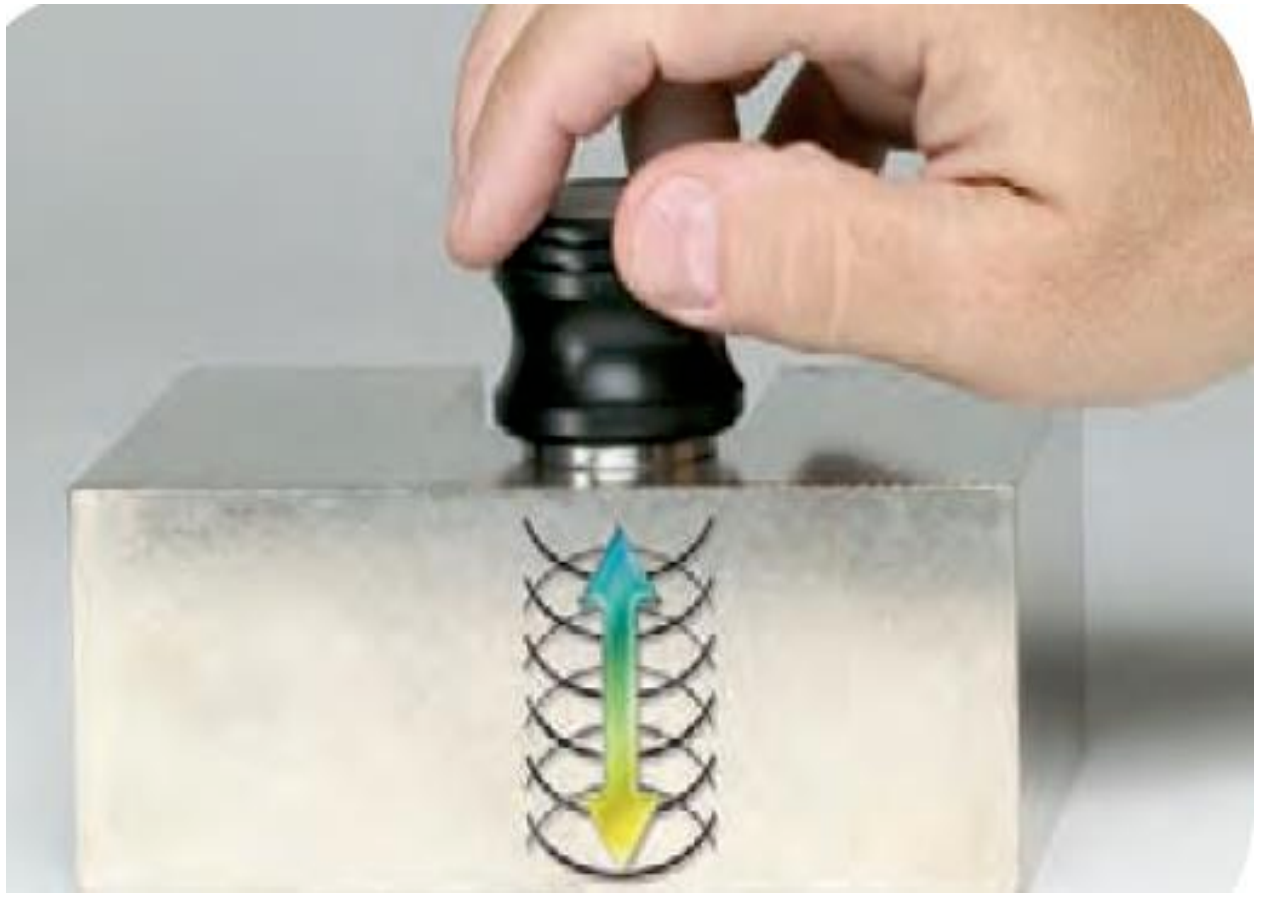
\includegraphics[width=\linewidth]{p03_img01.png}
  （a）接触式测试方法
\end{minipage}\hfill
\begin{minipage}[t]{0.48\textwidth}
  \centering
  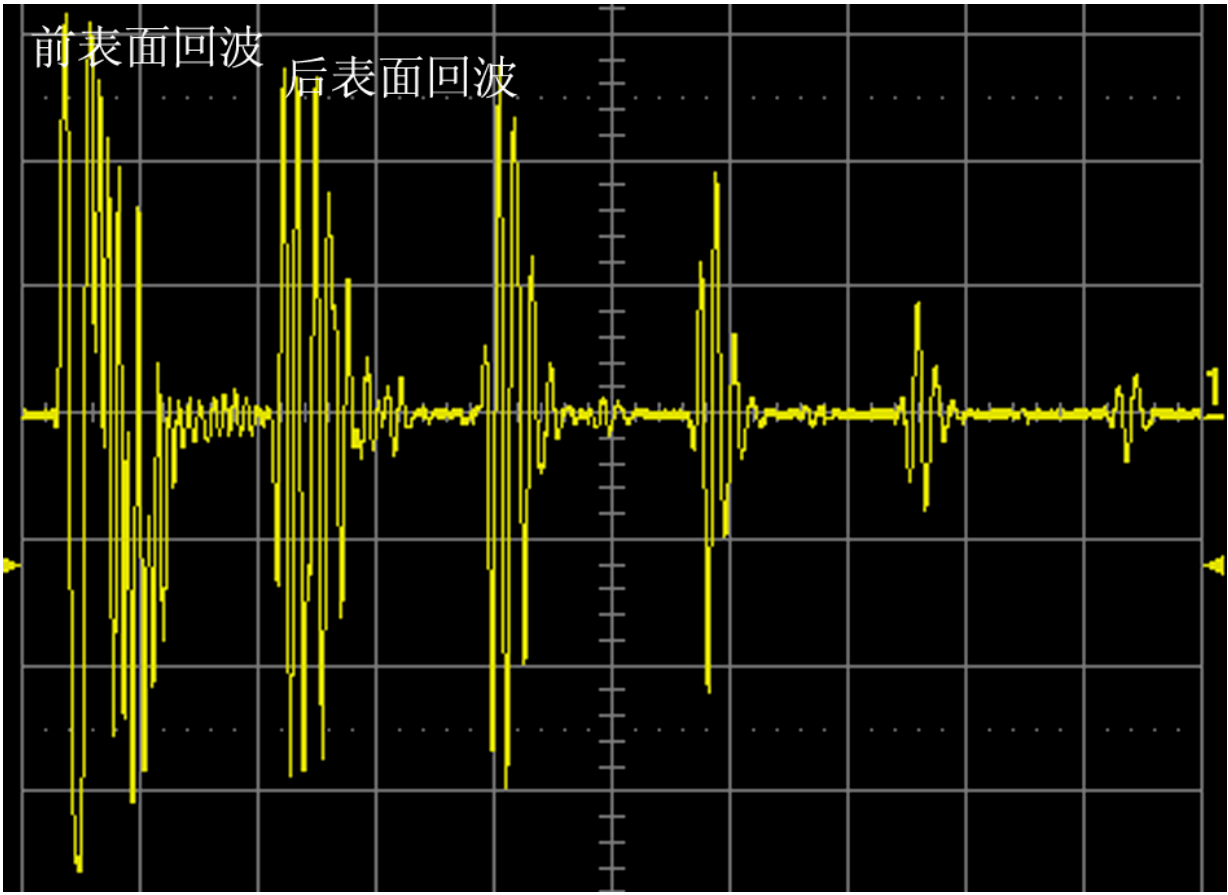
\includegraphics[width=\linewidth]{p03_img02.png}
  （b）测试信号
\end{minipage}
\caption{脉冲--回波方法}
\label{fig:exp2-pulse-echo}
\end{figure}

\subsubsection{波速}
根据回波信号得到两个回波峰值之间的时间差 $\Delta t$，并已知超声波传播路程 $\Delta L$ 为试件厚度 $d$ 的两倍，可计算出超声波的传播速度
\begin{equation}
  C=\frac{2d}{\Delta t}.
  \label{eq:exp2-speed}
\end{equation}

\subsubsection{衰减系数}
在介质中传播的超声平面波，其声压和声强振幅随传播距离 $x$ 的增加呈指数衰减，即
\begin{subequations}
\begin{align}
  P_x&=P_0e^{-\alpha x},\\
  I_x&=I_0e^{-2\alpha x}.
\end{align}
\end{subequations}
其中 $P$ 为声压，$I$ 为声强，$x$ 为声波传播的距离，$\alpha$ 为材料的衰减系数（单位为 NP/cm）。根据多次反射的回波信号，可以计算材料的衰减系数。对于任意两个回波 $n,m$（$n>m$），通过其峰值之间的幅值比可得到
\begin{equation}
  \alpha=\frac{1}{2(n-m)d}\ln\frac{P_m}{P_n}\quad(\mathrm{NP/cm}).
\end{equation}
实际测量中常采用 dB/cm 为单位，则衰减系数为
\begin{equation}
  \alpha=\frac{20}{2(n-m)d}\log_{10}\frac{|P_m|}{|P_n|}\quad(\mathrm{dB/cm}).
  \label{eq:exp2-attenuation}
\end{equation}
两种单位之间的换算关系为 $1\,\mathrm{NP/cm}=8.69\,\mathrm{dB/cm}$。

\subsubsection{材料常数（弹性模量和泊松比）}
根据无限弹性固体介质中波的传播特性，可得
\begin{subequations}
\begin{align}
  C_L&=\sqrt{\frac{E(1-\nu)}{\rho(1+\nu)(1-2\nu)}},\\
  C_S&=\sqrt{\frac{E}{2\rho(1+\nu)}}=\sqrt{\frac{G}{\rho}}.
\end{align}
\end{subequations}
通过测得材料中纵波和横波的波速 $C_L$ 和 $C_S$，即可得到材料的弹性模量和泊松比：
\begin{subequations}
\begin{align}
  \nu&=\frac{1-2(C_S/C_L)^2}{2-2(C_S/C_L)^2},\\
  E&=2\rho C_S^2(1+\nu).
  \label{eq:exp2-E}
\end{align}
\end{subequations}

\subsubsection{材料缺陷的检测}
如果知道试件厚度，可以通过测试波传播的时间差 $\Delta t$ 得到波速；反之，如果知道材料波速，可以通过测试前后表面波传播的时间差确定试件厚度，以及试件内部损伤的大小及位置。当超声波传播路径上无缺陷时，在探测信号入射波与底部回波之间不存在缺陷反射回波。当传播路径上存在缺陷，且缺陷界面小于探头晶片面积时，则同时存在缺陷反射回波和底面回波。当内部缺陷比较严重时，缺陷界面反射回波往往比较强，导致试件后表面无回波信号。因此，可以根据超声波反射回波特点对试件内部缺陷的位置及大小进行探测。

\begin{figure}[H]
  \centering
  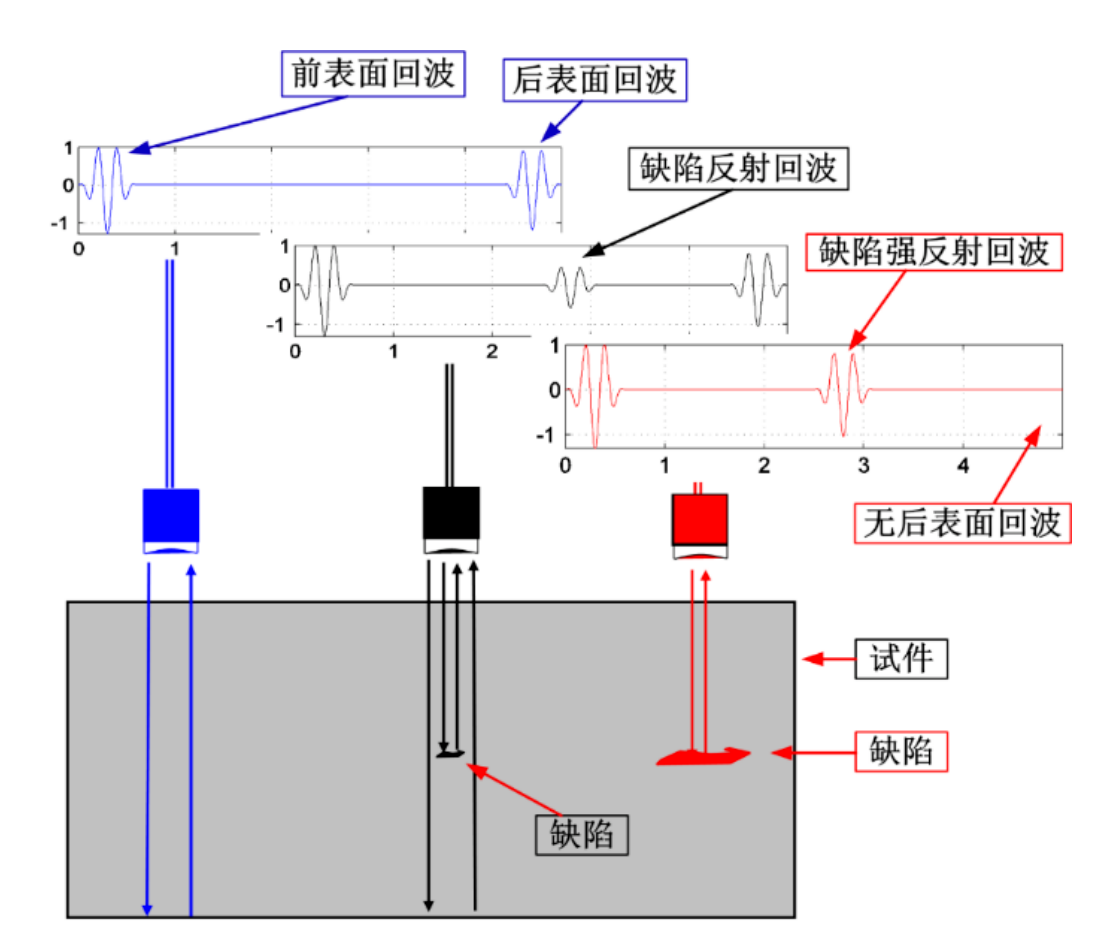
\includegraphics[width=0.5\textwidth]{p04_img01.png}
  \caption{有缺陷存在时波形示意图}
\end{figure}

超声波实验测试系统如图\ref{fig:exp2-system}所示。超声脉冲发射接收仪产生脉冲信号，通过超声探头转换为超声纵波或横波垂直入射到被测试件。同一探头接受试件底面反射的回波并转换为电信号，并采用数字存储示波器记录接收的信号进行分析。根据实验需要，可分别采用水浸式或接触式测试方式。超声纵波的测试两种方式都可以选择，只需选择对应探头；超声横波探头只能采用接触式测量。

\begin{figure}[H]
  \centering
  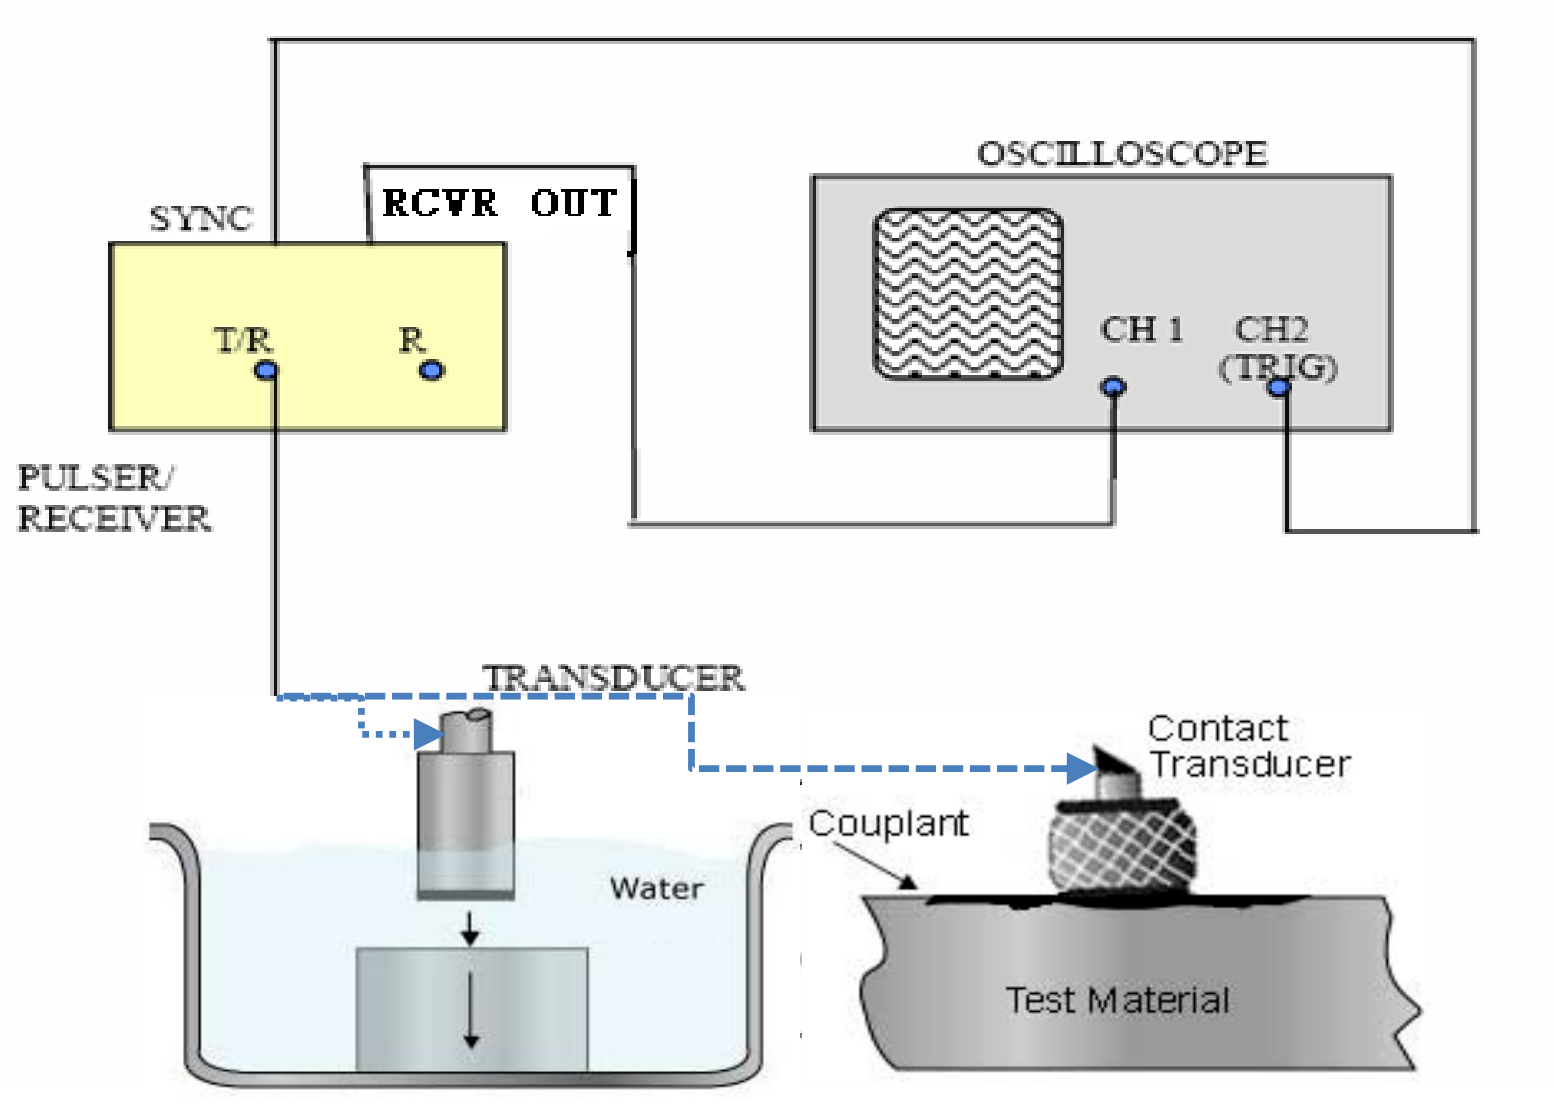
\includegraphics[width=0.7\textwidth]{p05_img01.png}
  \caption{实验测试系统示意图}
  \label{fig:exp2-system}
\end{figure}

\subsection{超声波实验测量的过程}
\subsubsection{材料密度测量}
分别测量钢、铝和有机玻璃试件的质量与尺寸，每个量记录一次，按试件形状计算密度。

\subsubsection{材料纵波波速和衰减系数测量}
\begin{enumerate}
  \item 实验准备：准备好装有足够水的水盆、酒精、脱脂棉等，并将水浸式超声探头架设在支架台上并探入水中。采用图\ref{fig:exp2-system}水浸式测量方式连接线路。
  \item 设置超声脉冲发射接收仪参数。
  \item 调节探头角度，使其垂直入射，测试超声波传播情况。测量探头距离盆底的距离，以便计算水的波速。
  \item 设置数字存储示波器参数，通过数字存储示波器采集超声探头接收的信号，并将数据及图像保存下来。
  \item 纵波波速测量：将钢、铝和有机玻璃分别放置于探头下，调整位置，进行测量。
  \item 数据分析：分析波形数据，得到所测材料的波速，并从多次反射峰值测超声波的衰减系数。
  \item 不同频率超声探头的纵波波速测量：采用纵波耦合剂接触式测量方式，分别采用 5 MHz 和 10 MHz 超声探头进行钢和有机玻璃的纵波波速测量。
  \item 不同频率超声探头的纵波衰减系数测量：采用纵波耦合剂接触式测量方式，分别采用 5 MHz 和 10 MHz 超声探头进行有机玻璃纵波衰减系数测量。
\end{enumerate}

\subsubsection{材料横波波速测量}
采用图\ref{fig:exp2-system}接触式测量方式连接线路，用酒精棉擦拭试件表面，将横波耦合剂涂于超声探头上，然后将横波超声探头与试件紧密接触，待信号稳定后采集并存储波形数据。所测试件分别为钢、铝和有机玻璃。

\subsubsection{钢板焊缝缺陷超声探测}
利用超声波脉冲回波模式，分别采用纵波超声直探头从钢板侧面垂直入射或斜探头从钢板表面斜入射的方式，对含焊缝钢板进行 B-Scan 超声探测，分析焊缝缺陷的位置及大小。
\begin{enumerate}
  \item 根据图\ref{fig:exp2-weld-setup}建立探测系统，选择探测模式，调节仪器参数。
  \item 在钢板侧面和表面画好探测路径并标好刻度，涂上纵波耦合剂。
  \item 在已画好的探测路径上每隔 0.5 cm 或 1 cm 进行一次超声探测，利用示波器和计算机进行信号数据采集存储。
  \item 通过分析所采集的信号，判断焊缝缺陷的位置和大小。
  \item 在钢板侧面纵波探测结果的基础上，在表面沿着与焊缝平行的方向，采用斜探头进行焊缝损伤的再次检测，并与前面的结果进行比较、分析。
\end{enumerate}

\begin{figure}[H]
  \centering
  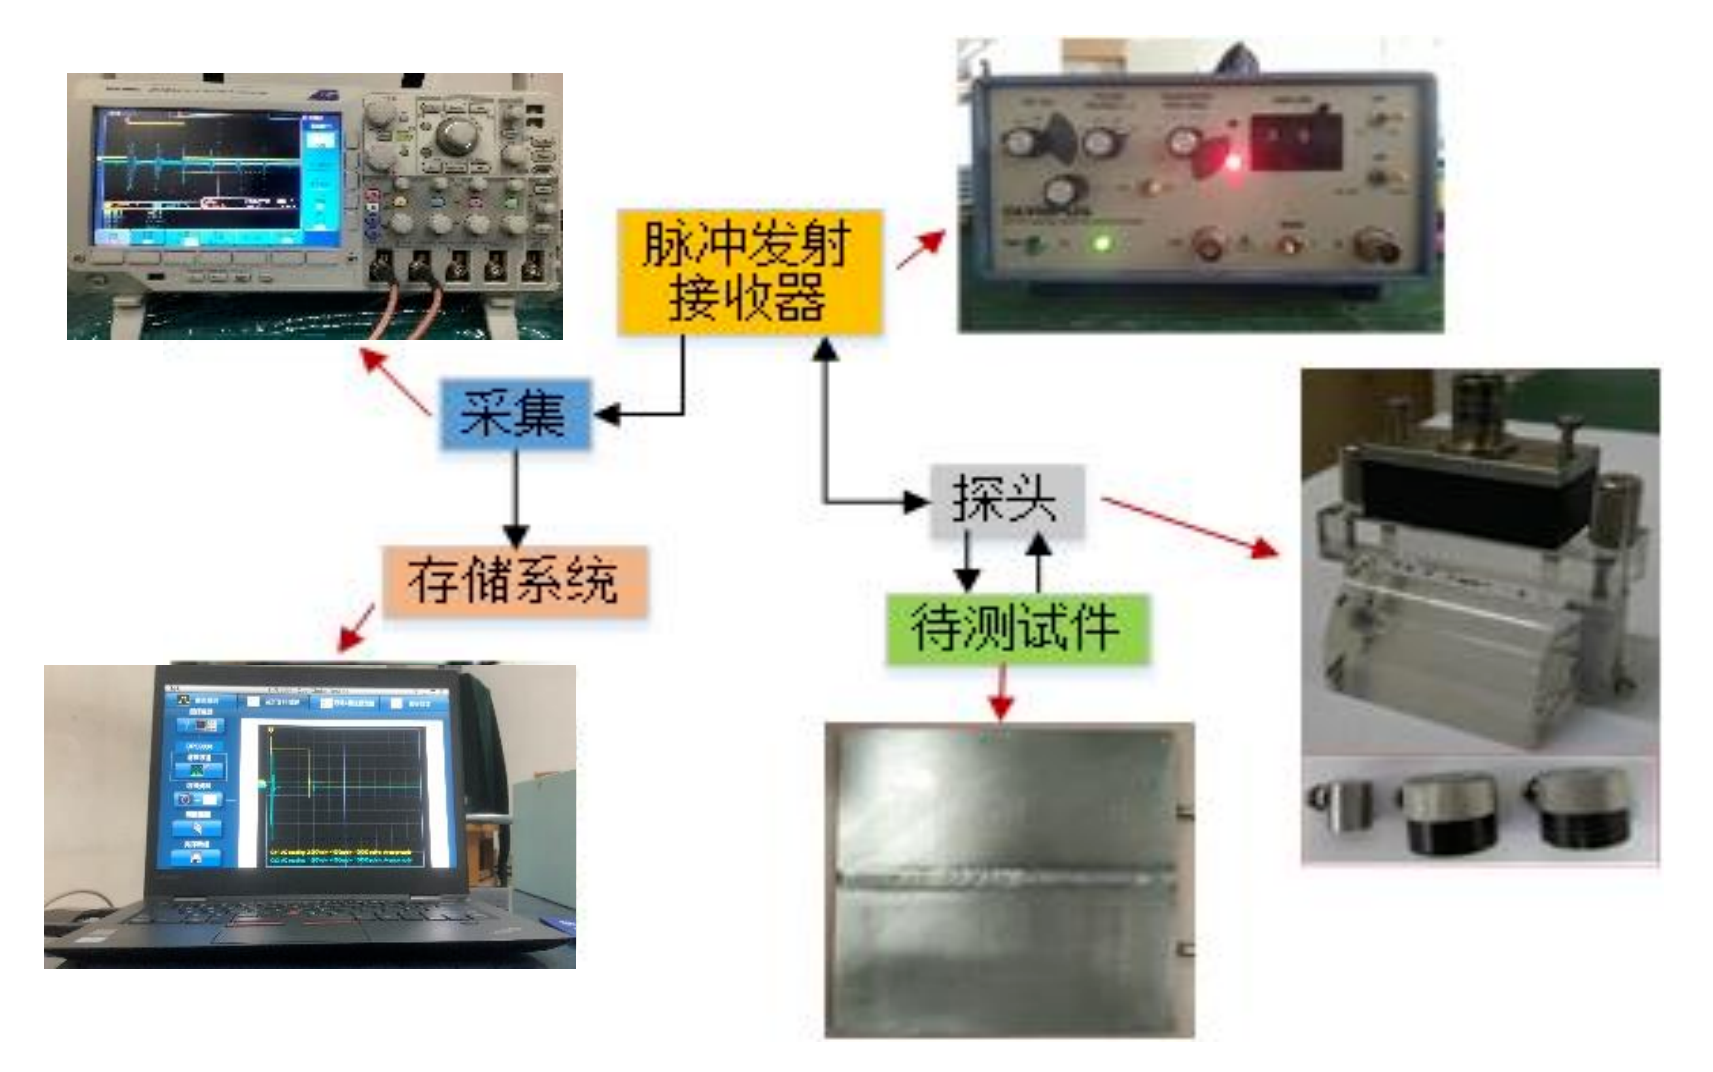
\includegraphics[width=0.75\textwidth]{p06_img01.png}
  \caption{钢板焊缝损伤检测}
  \label{fig:exp2-weld-setup}
\end{figure}

\section{脉冲--回波法测量波速和衰减系数、弹性模量和泊松比}
\noindent\textbf{填写说明：}本部分信号图均为本组实测波形；试件质量、尺寸及探头与盆底距离均为本组现场读数；时间差、回波幅值及各计算结果均已填写。探伤部分结果与图像均已按本组记录填写。

\subsection{材料密度测量}
钢、铝试件按圆柱体处理，有机玻璃试件按长方体处理。每个质量和尺寸量只读取一次，记录在表\ref{tab:exp2-density}。质量以 g、尺寸以 mm 记录，计算密度时换算为 $\mathrm{g/cm^3}$。

\begin{table}[H]
\centering
\caption{试件质量和尺寸的单次测量结果}
\label{tab:exp2-density}
\begin{tabular}{llc}
\toprule
试件 & 测量量 & 读数\\
\midrule
\multirow{3}{*}{钢} & 质量 $m_{st}$（g） & 81.943\\
 & 直径 $d_{st}$（mm） & 29.8\\
 & 厚度 $h_{st}$（mm） & 15.05\\
\midrule
\multirow{3}{*}{铝} & 质量 $m_{al}$（g） & 29.468\\
 & 直径 $d_{al}$（mm） & 30.0\\
 & 厚度 $h_{al}$（mm） & 15.02\\
\midrule
\multirow{4}{*}{有机玻璃} & 质量 $m_{og}$（g） & 131.189\\
 & 长度 $a_{og}$（mm） & 98.9\\
 & 宽度 $b_{og}$（mm） & 80.4\\
 & 厚度 $h_{og}$（mm） & 14.1\\
\bottomrule
\end{tabular}
\end{table}

由质量和几何体积计算密度。将表中以 mm 记录的尺寸直接代入时，单位换算系数为 $10^3$：
\begin{subequations}
\begin{align}
  \rho_{st}&=\frac{4\times10^3m_{st}}{\pi d_{st}^{\,2}h_{st}}
  =7.806\ \mathrm{g/cm^3},\\
  \rho_{al}&=\frac{4\times10^3m_{al}}{\pi d_{al}^{\,2}h_{al}}
  =2.776\ \mathrm{g/cm^3},\\
  \rho_{og}&=\frac{10^3m_{og}}{a_{og}b_{og}h_{og}}
  =1.170\ \mathrm{g/cm^3}.
\end{align}
\end{subequations}

\subsection{水的纵波波速}
将频率为 5 MHz 的水浸式超声探头浸入水中并调整角度，使探头垂直入射。选用合适大小的试件固定探头和盆底的距离，之后取出试件并测量其厚度，即为探头与底部的距离 $h$。在示波器波形中读取入射波与反射波之间的时间差 $\Delta t$，由式\eqref{eq:exp2-speed}计算水中波速。信号图见图\ref{fig:exp2-water-signal}。

\begin{table}[H]
\centering
\caption{测量水中纵波波速时探头与盆底的距离}
\label{tab:exp2-water-distance}
\begin{tabular}{lc}
\toprule
测量量 & 单次读数\\
\midrule
距离 $h$（mm） & 50\\
\bottomrule
\end{tabular}
\end{table}

\begin{figure}[H]
\centering
\begin{minipage}[t]{0.48\textwidth}
  \centering
  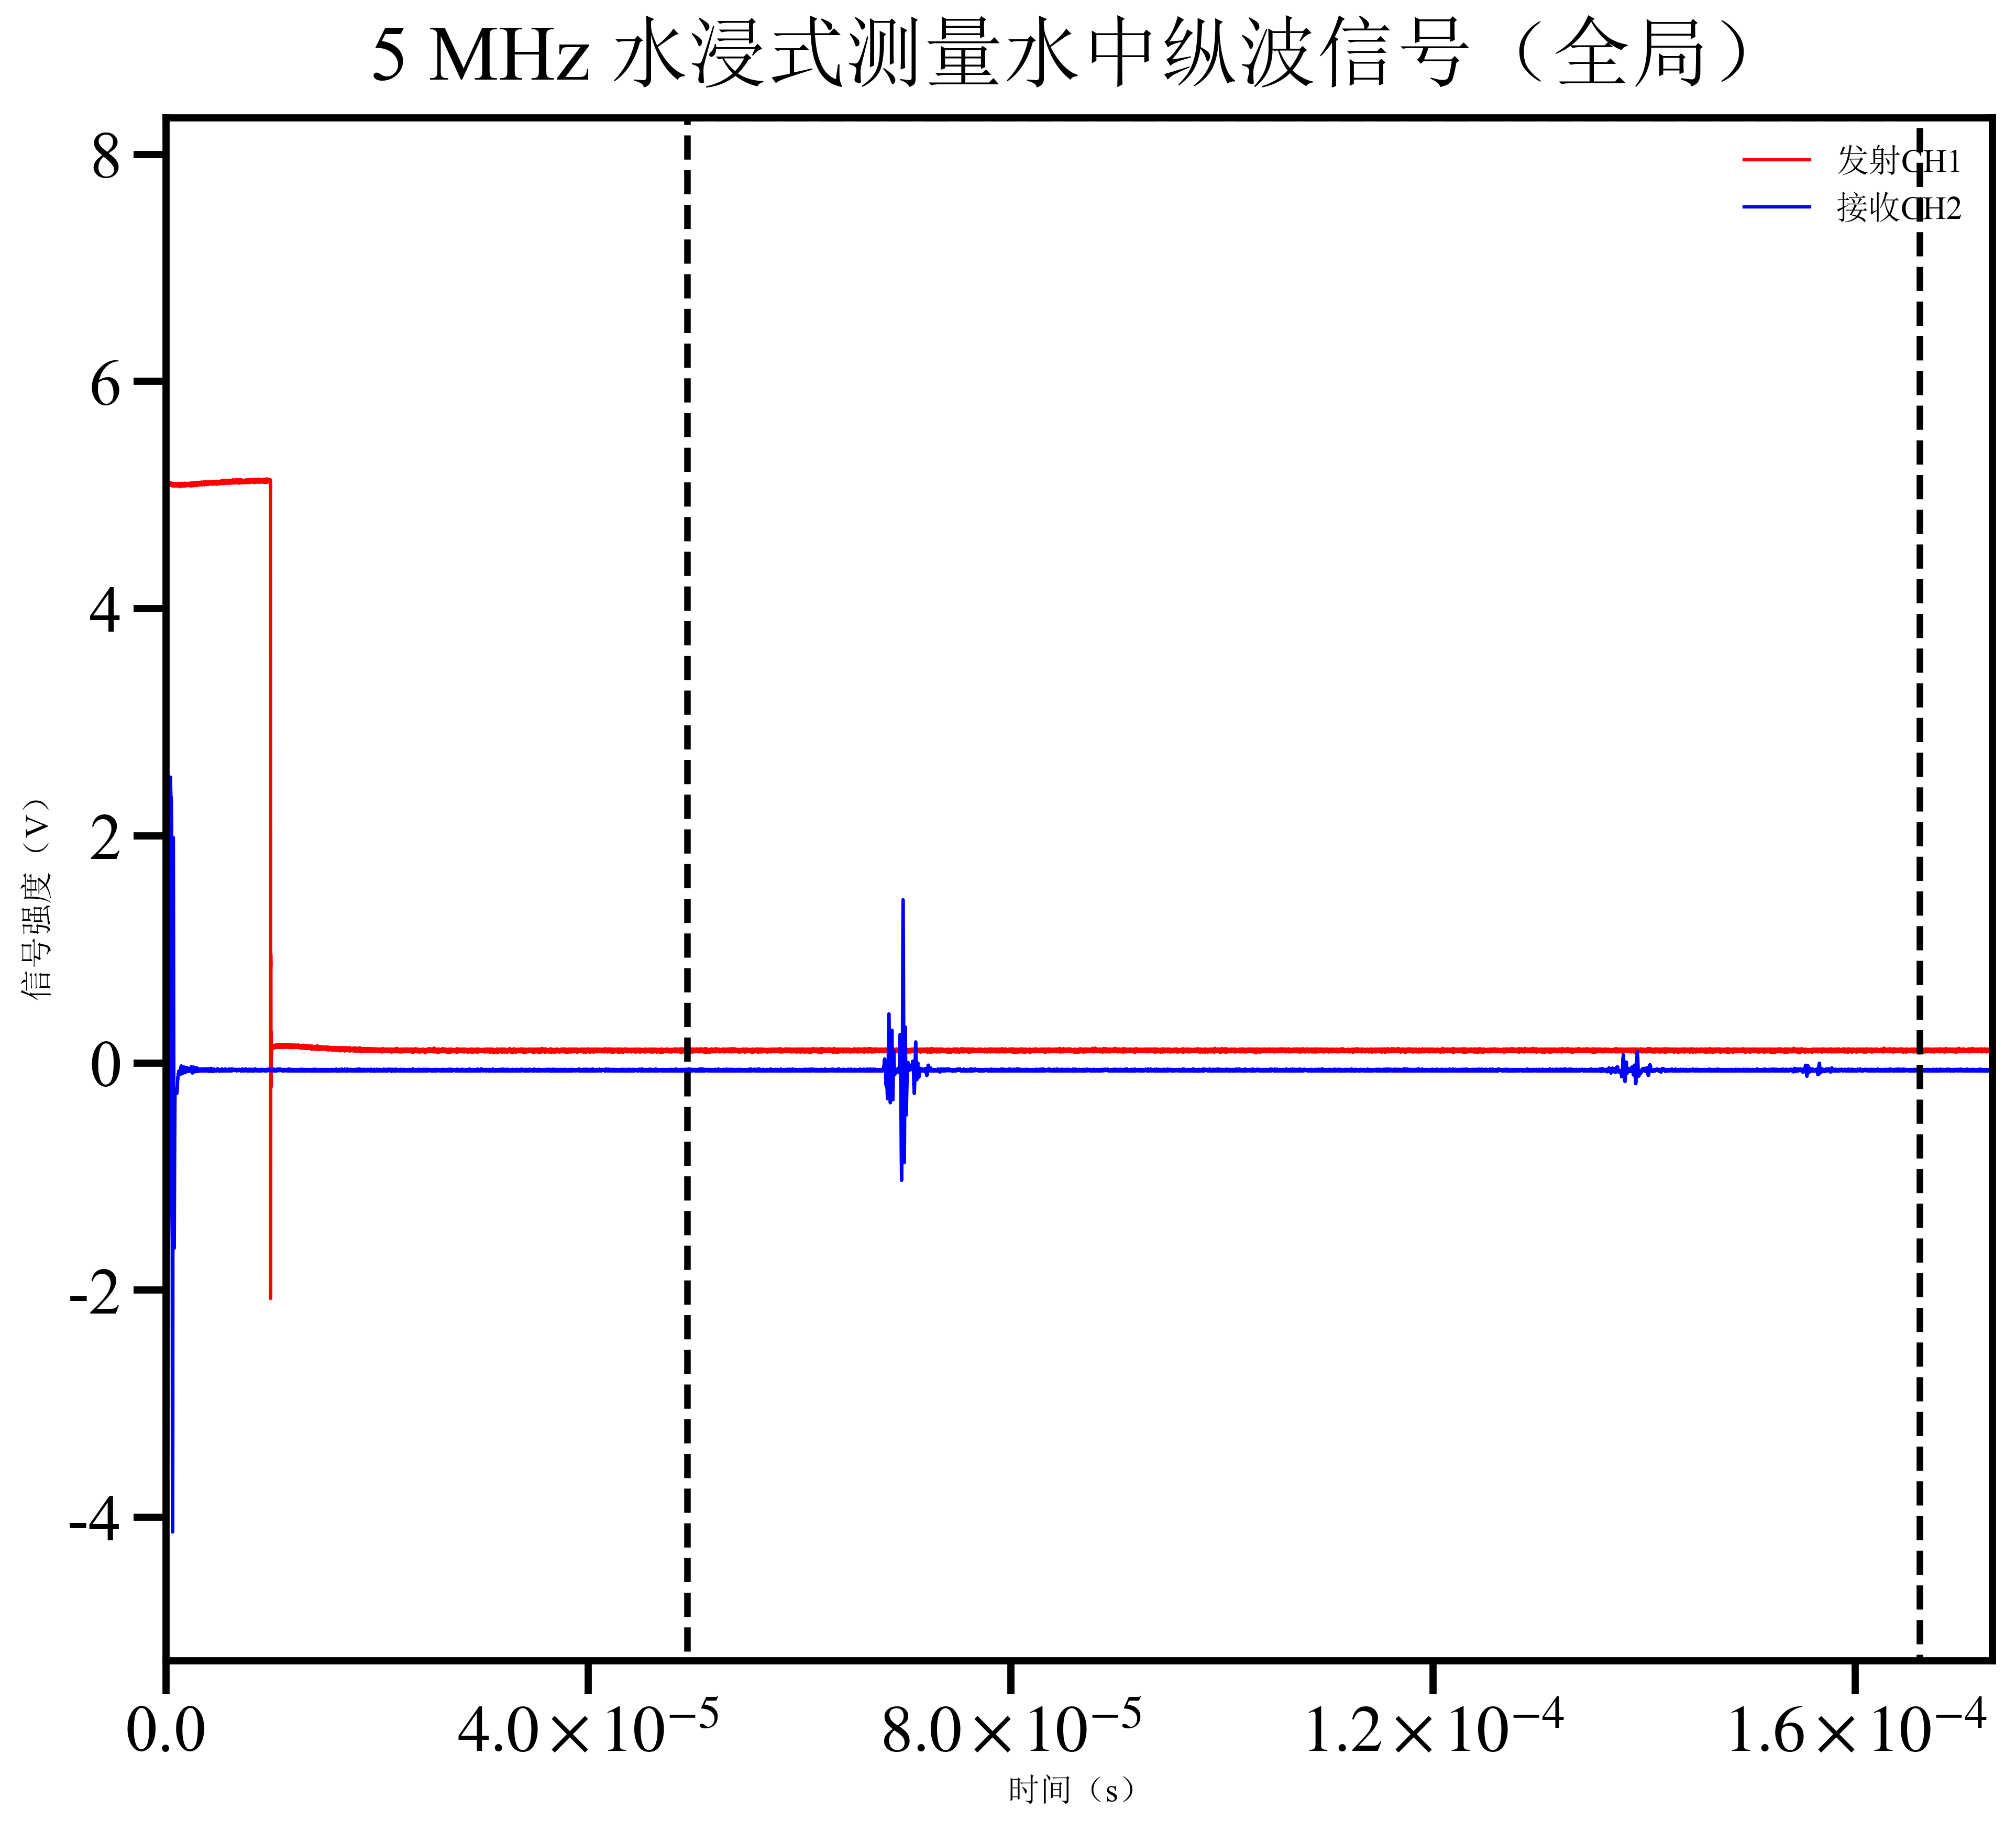
\includegraphics[width=\linewidth]{water_global.png}
  （a）输入输出信号全局图
\end{minipage}\hfill
\begin{minipage}[t]{0.48\textwidth}
  \centering
  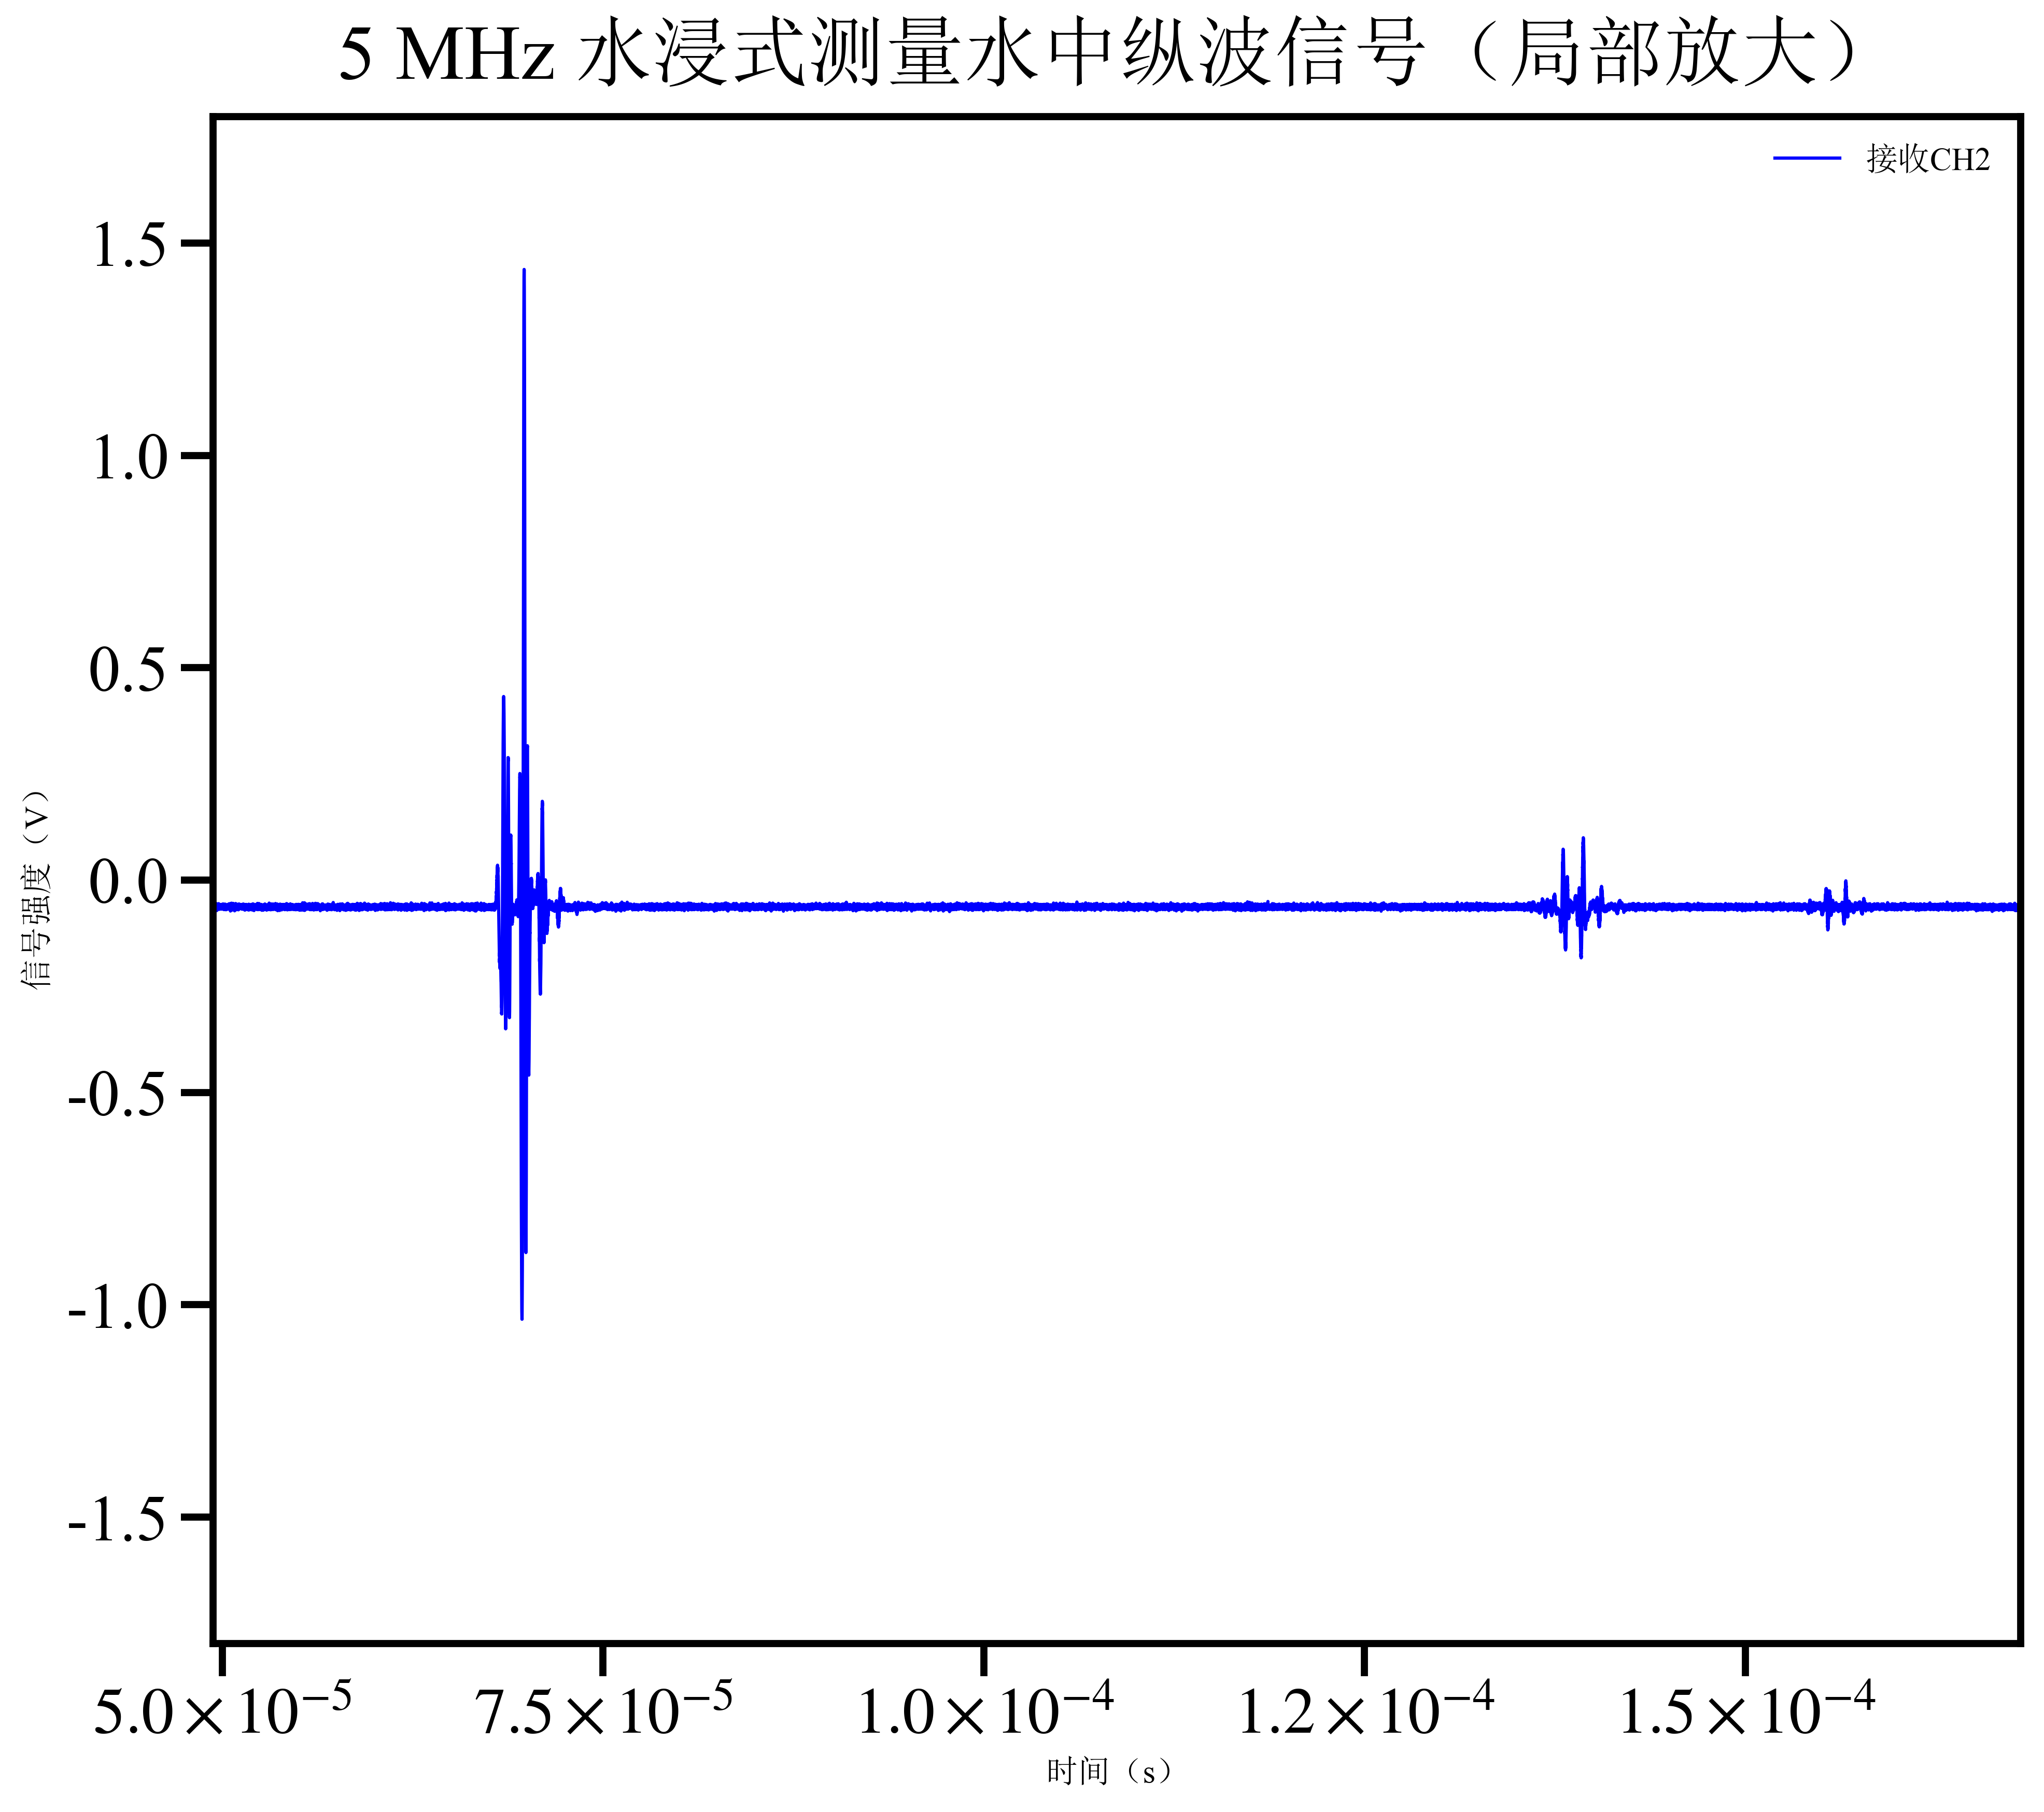
\includegraphics[width=\linewidth]{water_zoom.png}
  （b）输出信号局部放大图
\end{minipage}
\caption{5 MHz 测量水中纵波波速时信号图}
\label{fig:exp2-water-signal}
\end{figure}

\begin{table}[H]
\centering
\caption{5 MHz 测量水中纵波波速时的时间差}
\label{tab:exp2-water-time}
\begin{tabular}{lc}
\toprule
测量量 & 单次读数\\
\midrule
$\Delta t$（$\mu$s） & 69.81\\
\bottomrule
\end{tabular}
\end{table}

表\ref{tab:exp2-water-distance}中的 $h$ 以 mm 记录，表\ref{tab:exp2-water-time}中的 $\Delta t$ 以 $\mu$s 记录，故水中纵波波速为
\begin{equation}
  C_{water}=\frac{2h}{\Delta t}\times10^3
  =1432\ \mathrm{m/s}.
\end{equation}
常温水中的超声波波速参考值取 $1480\,\mathrm{m/s}$，相对误差为
\begin{equation}
  \delta_{water}=\frac{|C_{water}-1480|}{1480}\times100\%
  =3.2\%.
\end{equation}
分析距离测量、探头移动及时间差读数等因素对结果的影响。
本组波形中盆底回波清晰，入射波与回波之间几乎无杂波。时间差读数的不确定性主要来自波峰位置的选取：取波包前沿与主峰对应的时间可相差约 $1\,\mu$s，折算波速差异约 1\%。距离 $h$ 为游标卡尺单次测量，探头与盆底是否严格垂直、取出固定试件时探头是否发生移动，是本项测量的主要系统误差来源。

\subsection{水浸式测量三种材料的纵波波速}
利用频率为 5 MHz 的水浸式超声探头测量纵波在钢、铝、有机玻璃中的传播速度。将试件依次放入水中，调整探头方向使其垂直于试件表面，待示波器信号稳定后记录并导出数据。波形及用于计算波速的数据区域如图\ref{fig:exp2-steel-L}--图\ref{fig:exp2-og-L}所示，波峰时间差填入表\ref{tab:exp2-L-time}。

\begin{figure}[H]
\centering
\begin{minipage}[t]{0.48\textwidth}
  \centering
  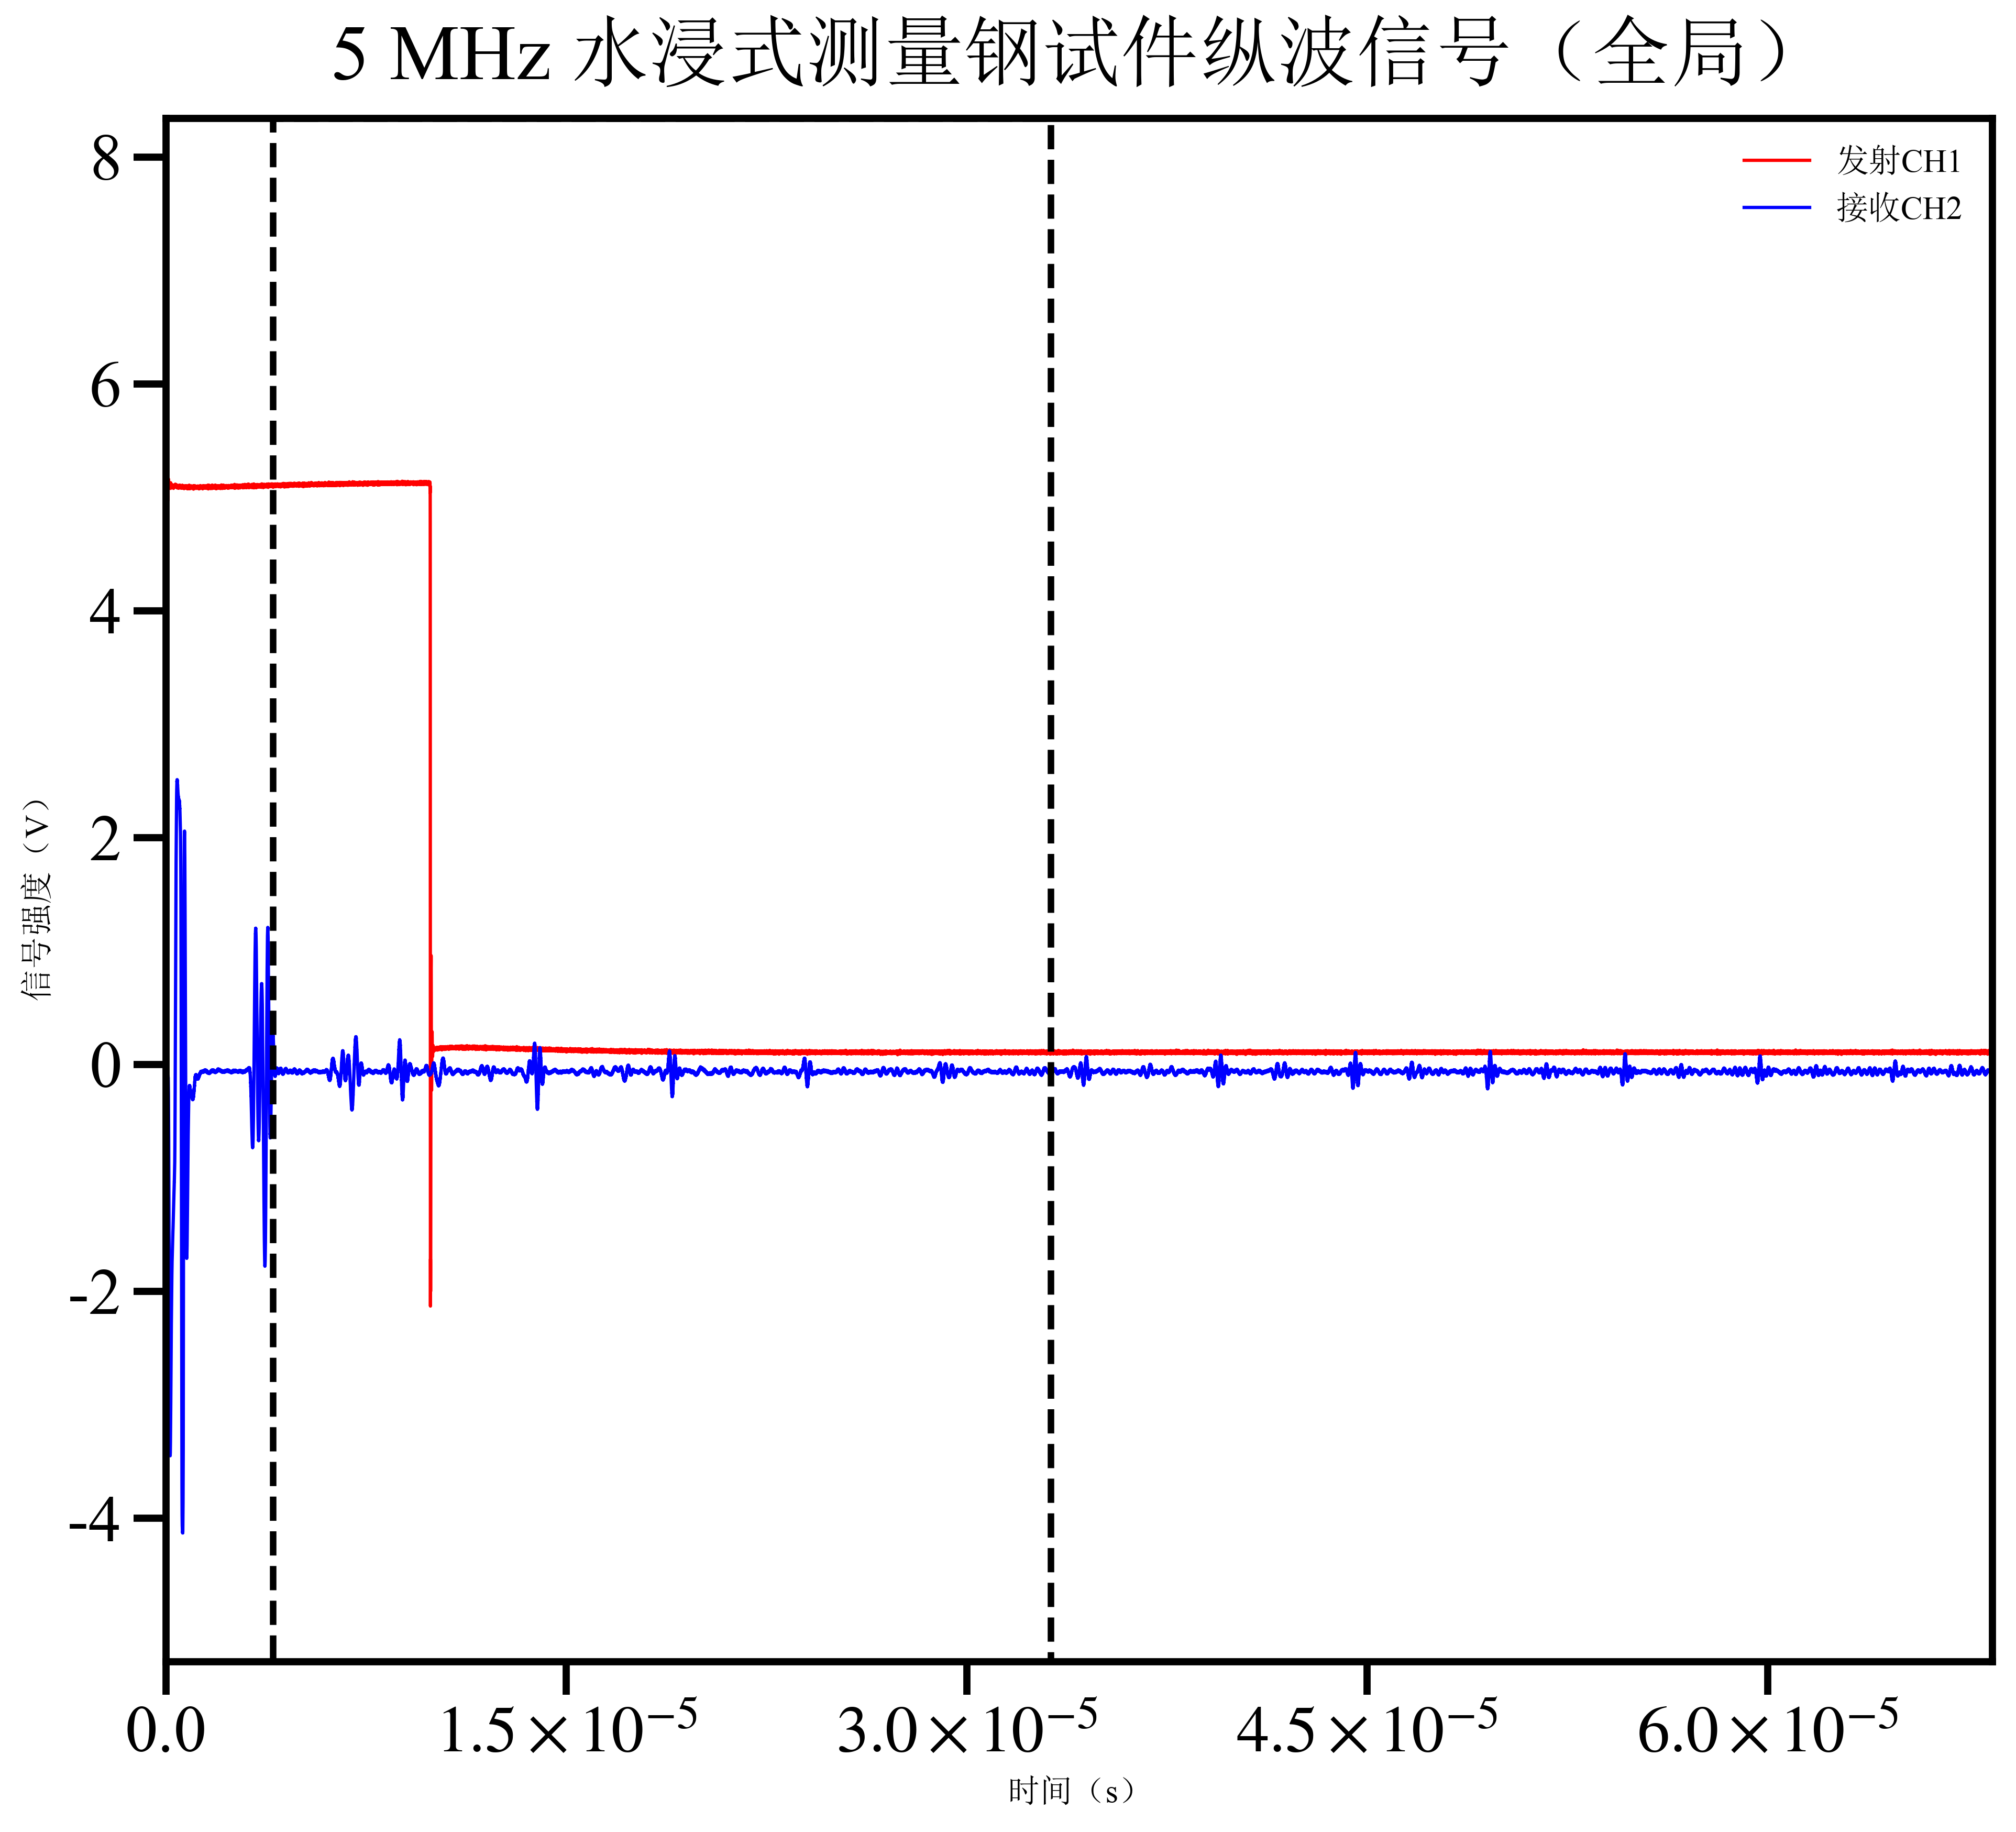
\includegraphics[width=\linewidth]{steel_water_global.png}
  （a）输入输出信号全局图
\end{minipage}\hfill
\begin{minipage}[t]{0.48\textwidth}
  \centering
  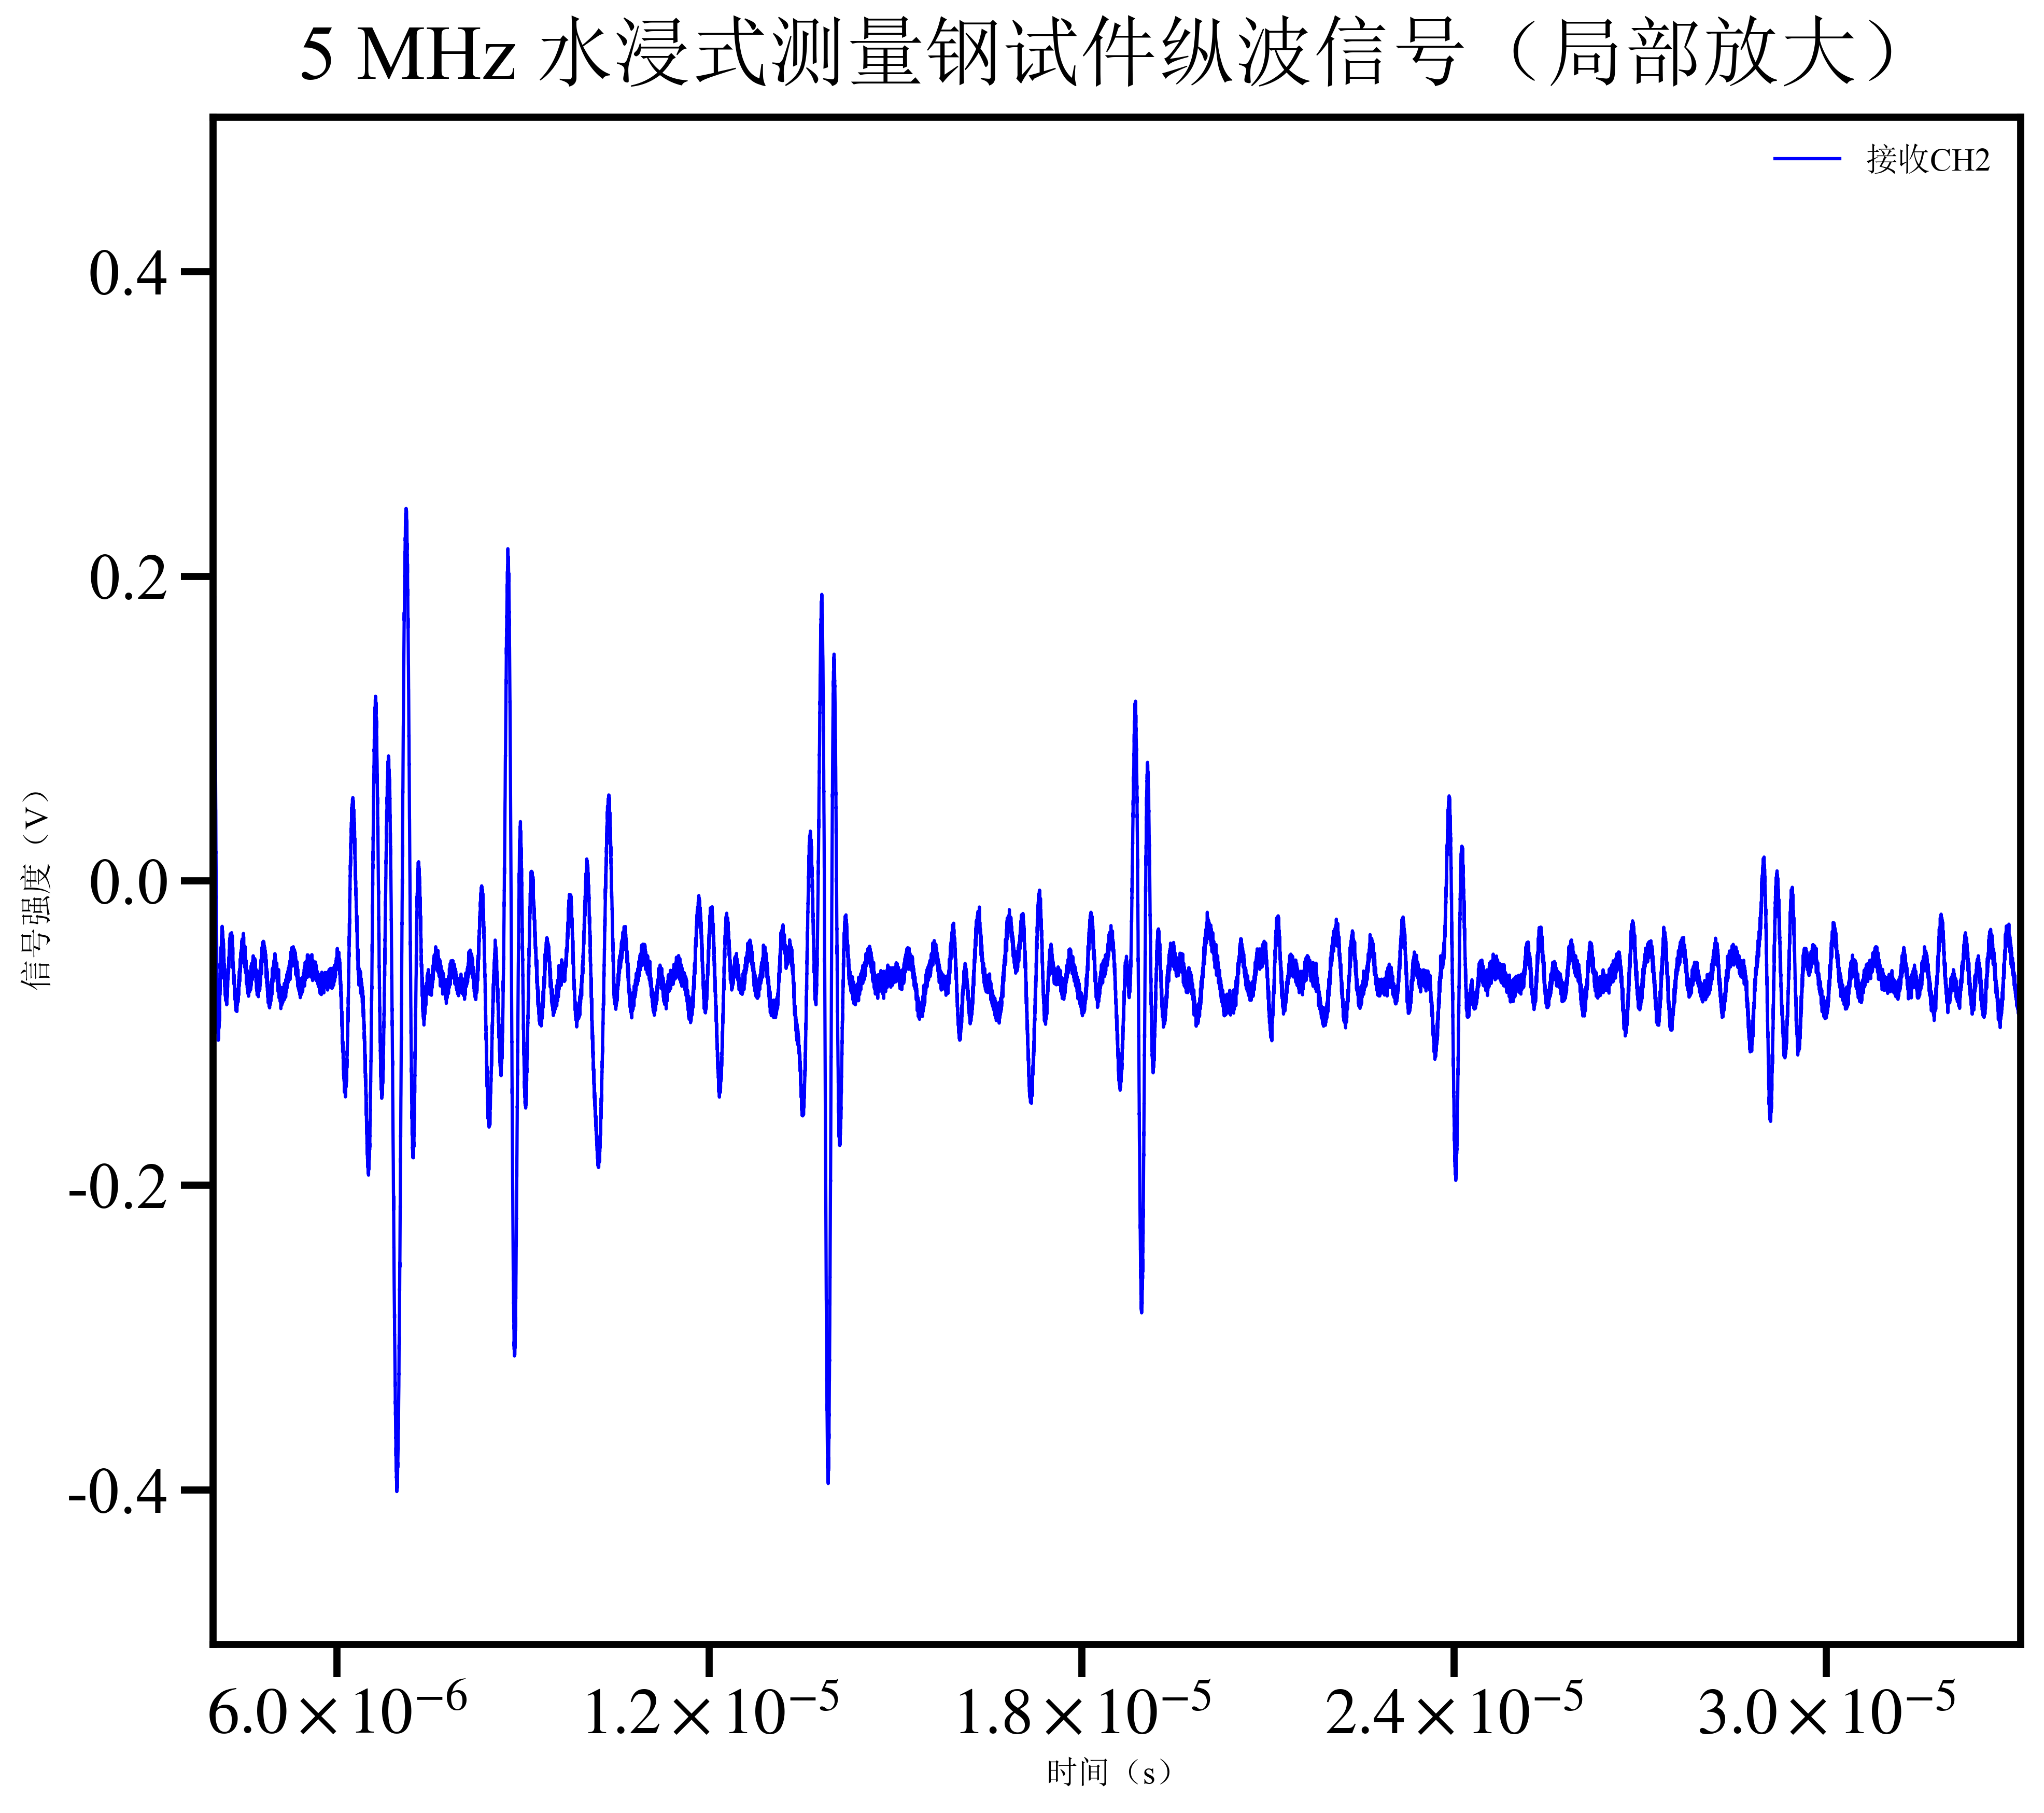
\includegraphics[width=\linewidth]{steel_water_zoom.png}
  （b）输出信号局部放大图
\end{minipage}
\caption{5 MHz 水浸式测量钢试件纵波波速时信号图}
\label{fig:exp2-steel-L}
\end{figure}

\begin{figure}[H]
\centering
\begin{minipage}[t]{0.48\textwidth}
  \centering
  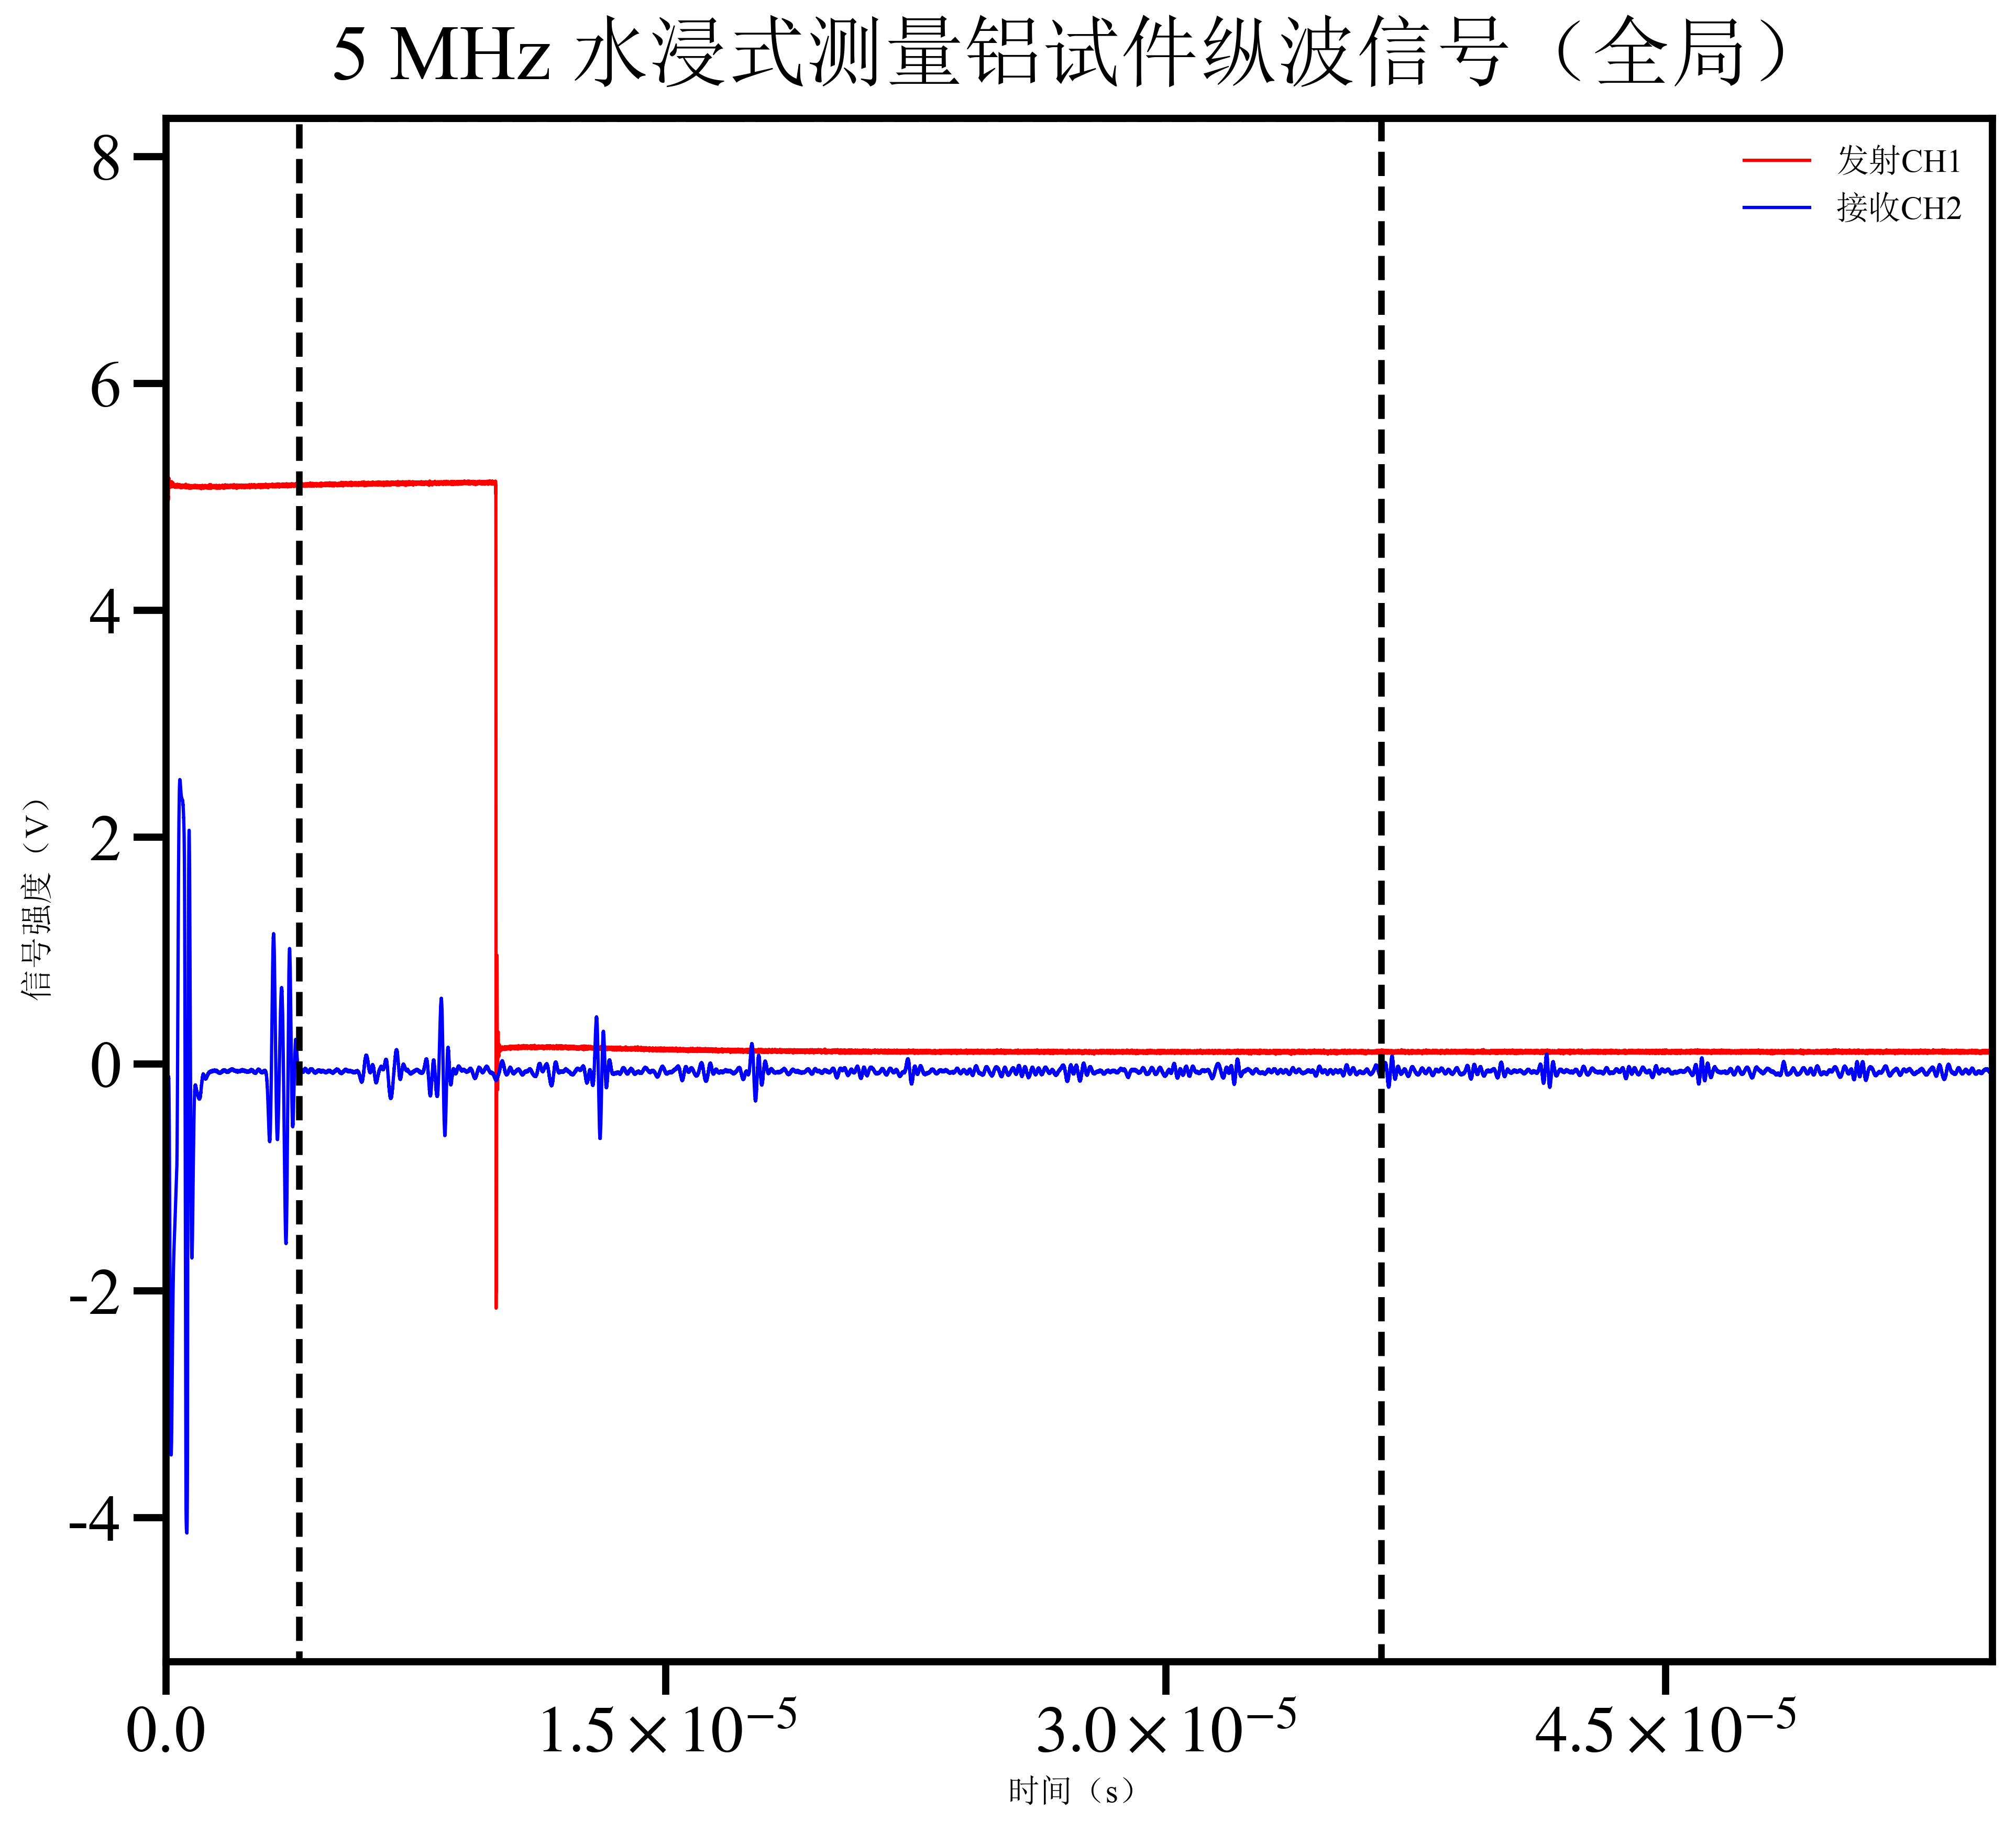
\includegraphics[width=\linewidth]{alu_water_global.png}
  （a）输入输出信号全局图
\end{minipage}\hfill
\begin{minipage}[t]{0.48\textwidth}
  \centering
  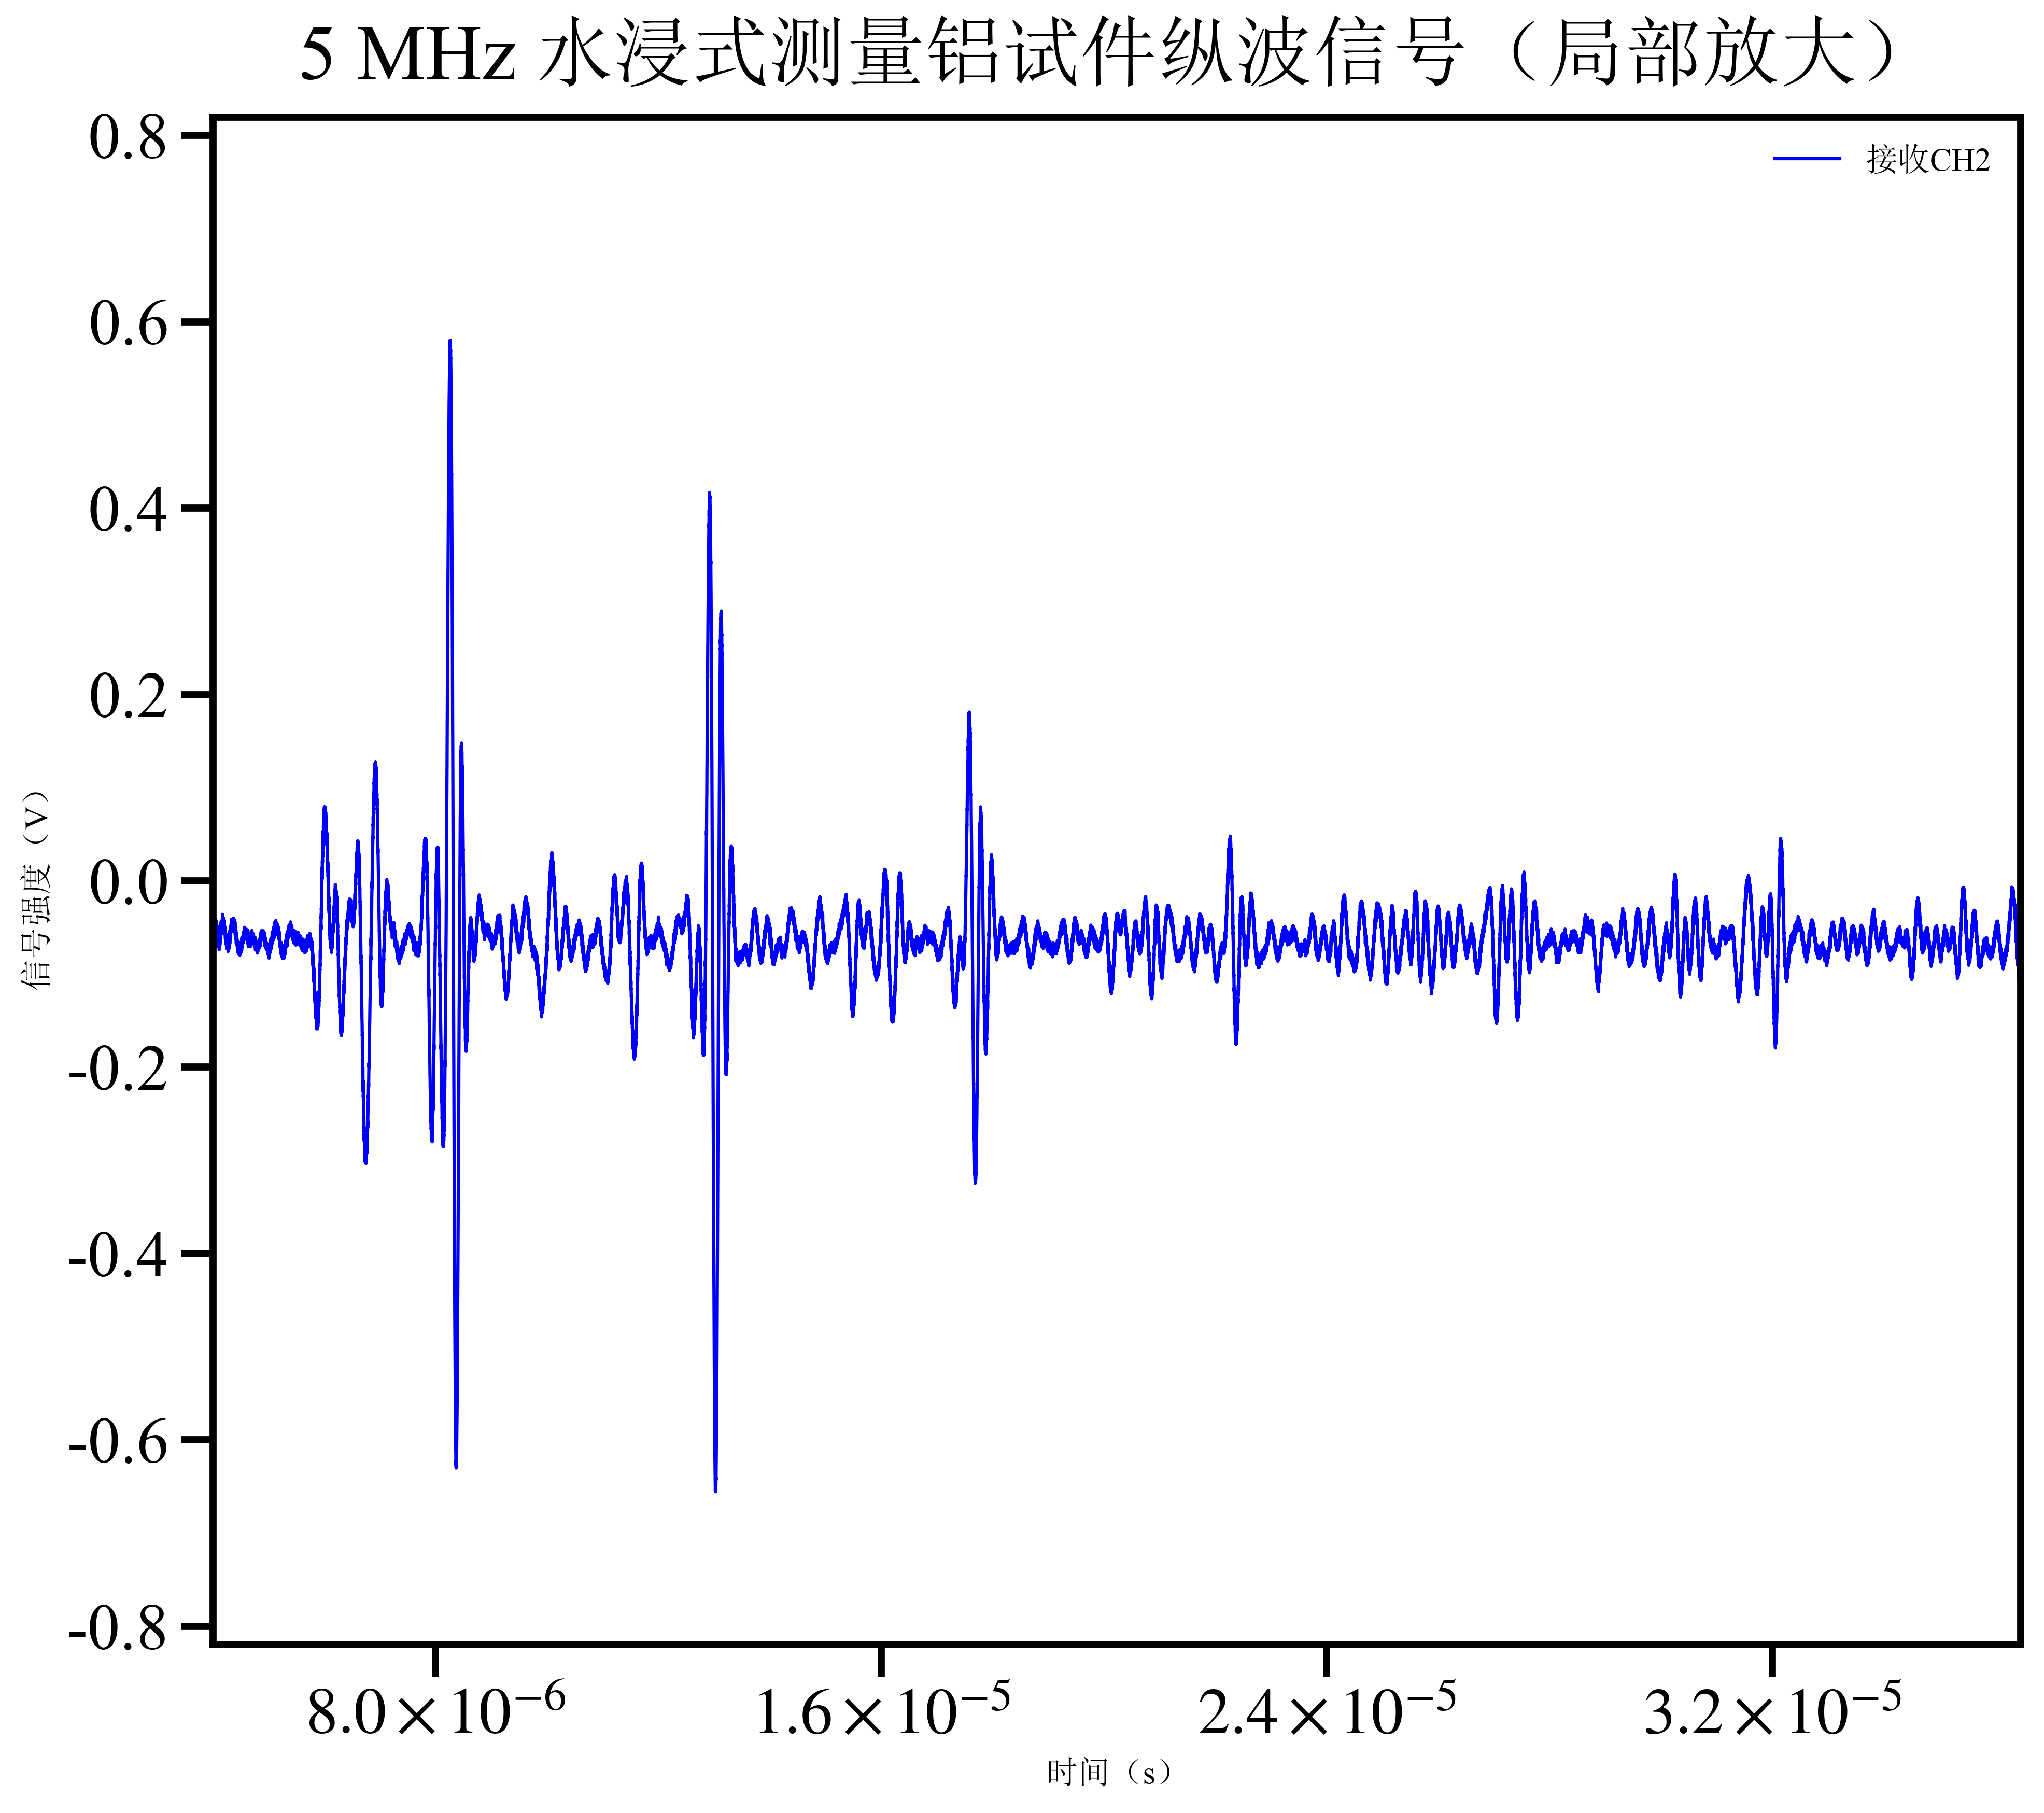
\includegraphics[width=\linewidth]{alu_water_zoom.png}
  （b）输出信号局部放大图
\end{minipage}
\caption{5 MHz 水浸式测量铝试件纵波波速时信号图}
\end{figure}

\begin{figure}[H]
\centering
\begin{minipage}[t]{0.48\textwidth}
  \centering
  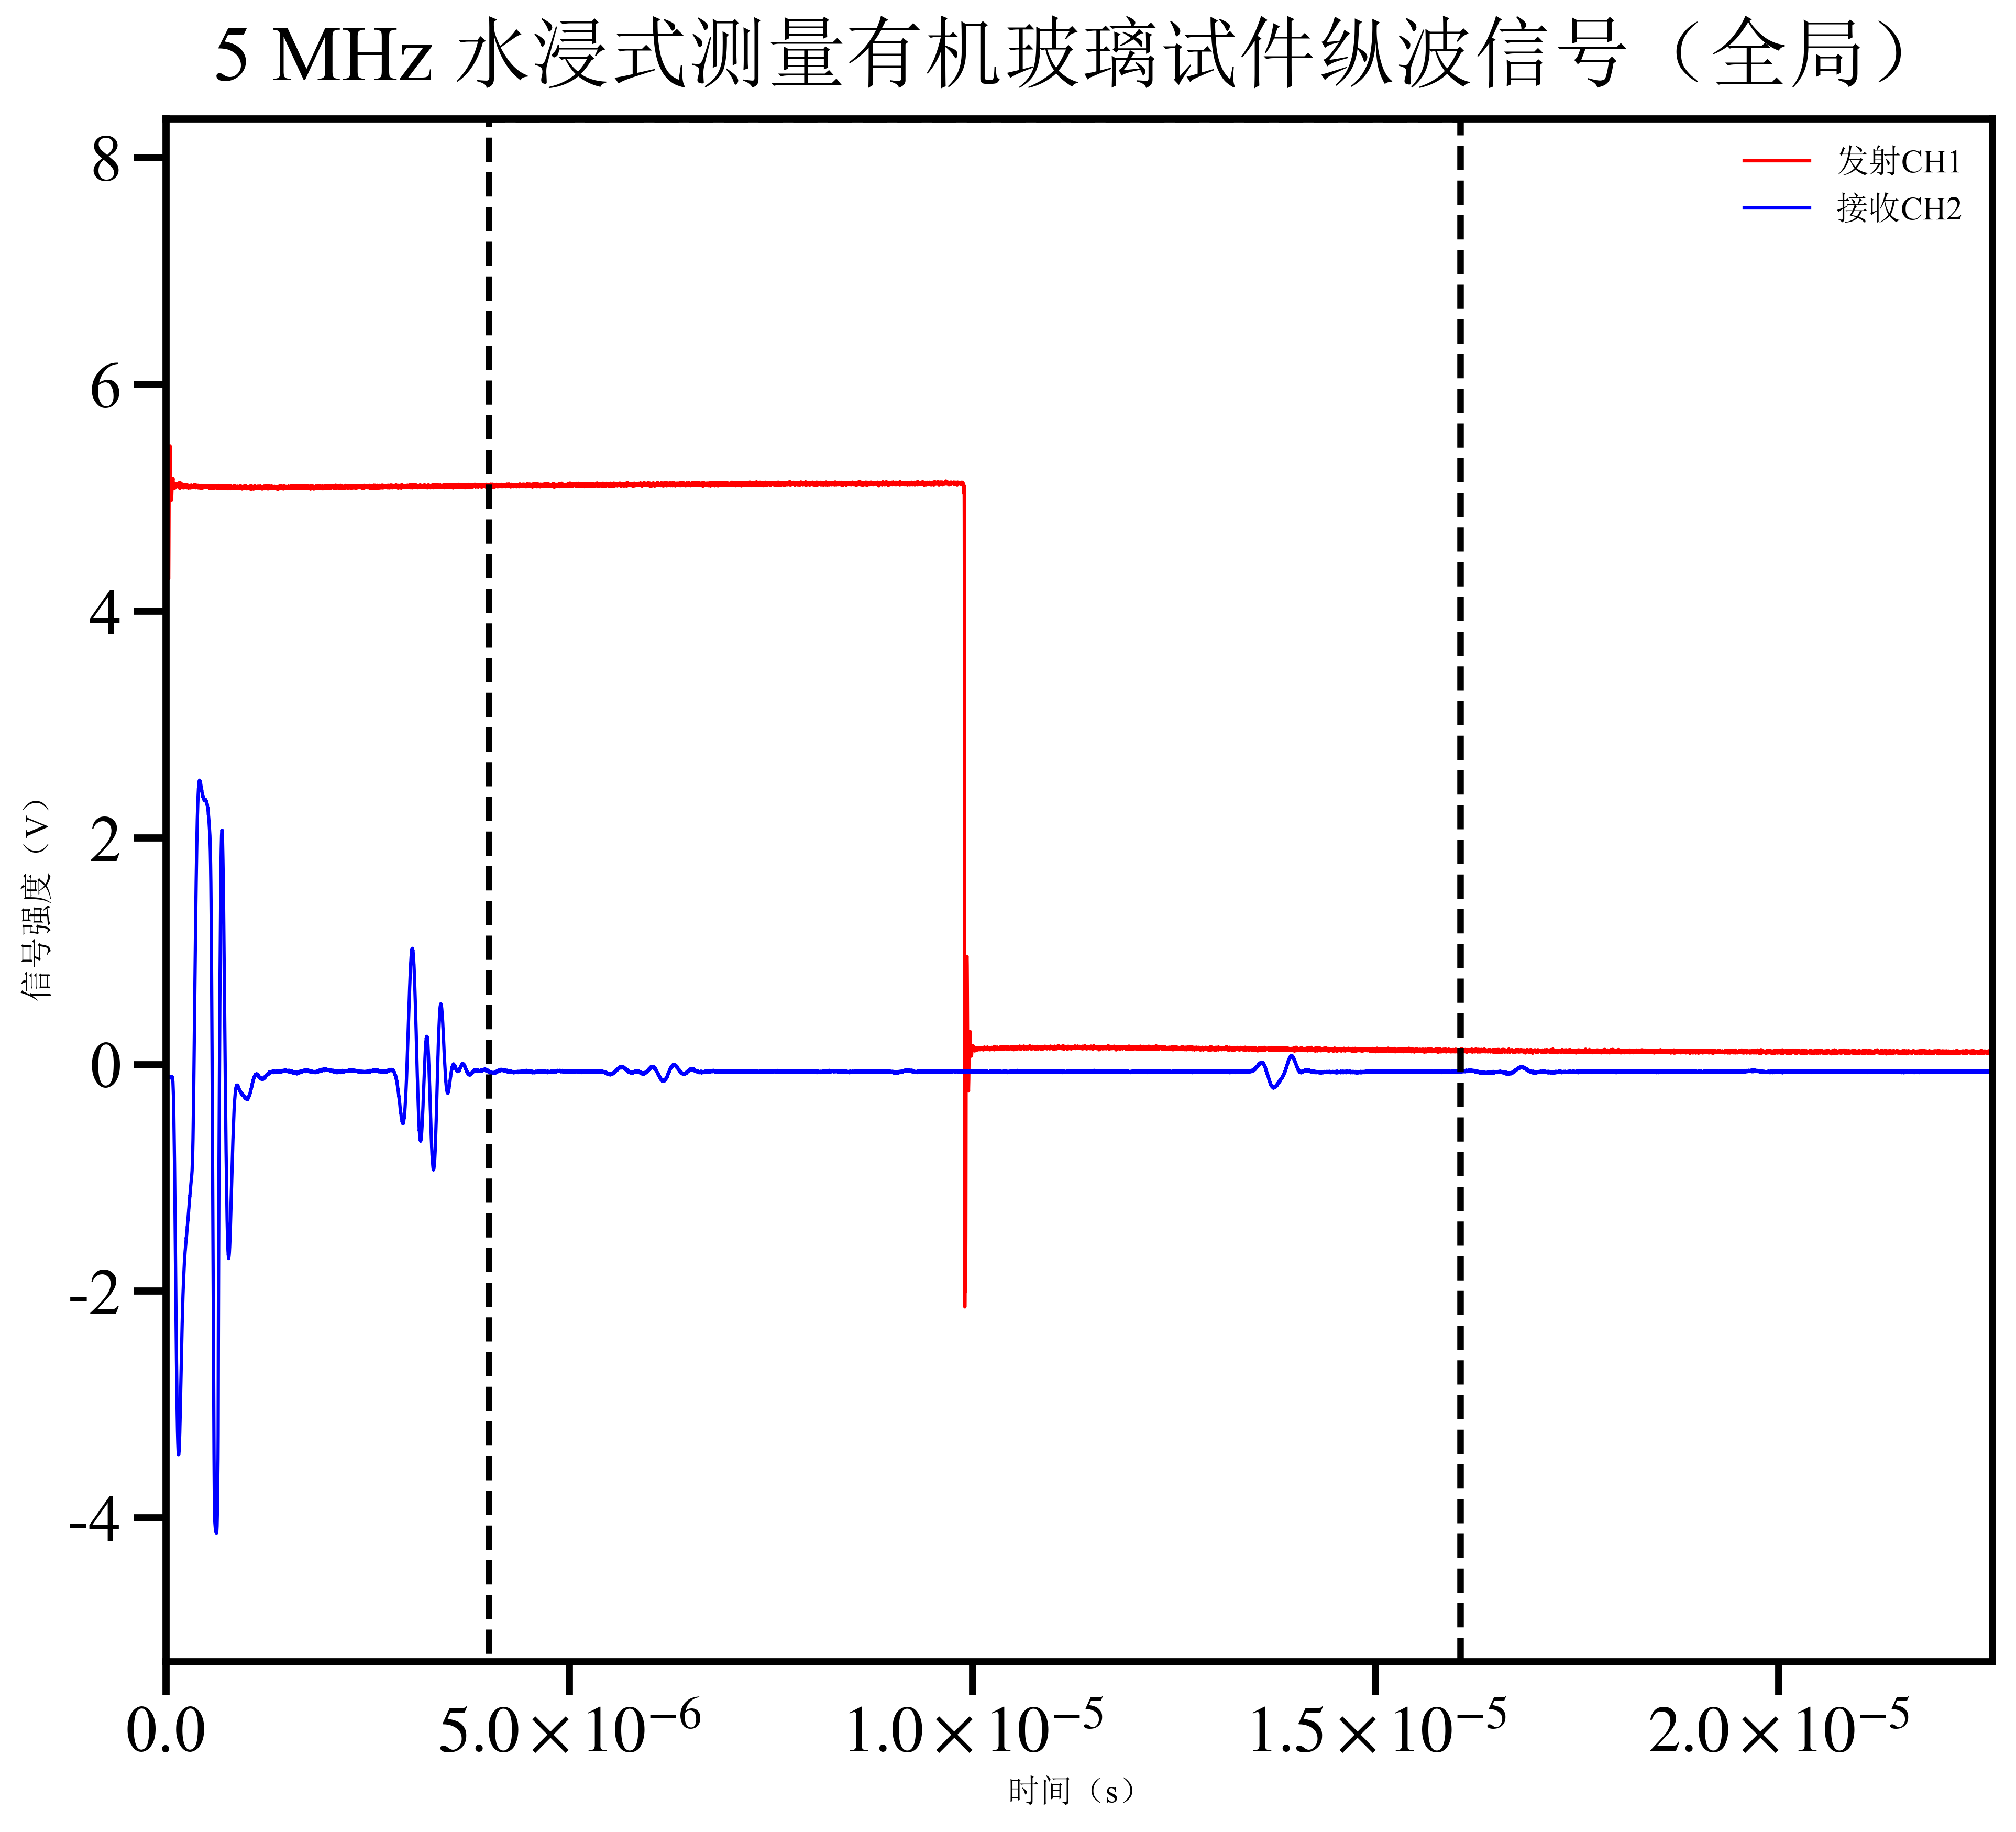
\includegraphics[width=\linewidth]{glass_water_global.png}
  （a）输入输出信号全局图
\end{minipage}\hfill
\begin{minipage}[t]{0.48\textwidth}
  \centering
  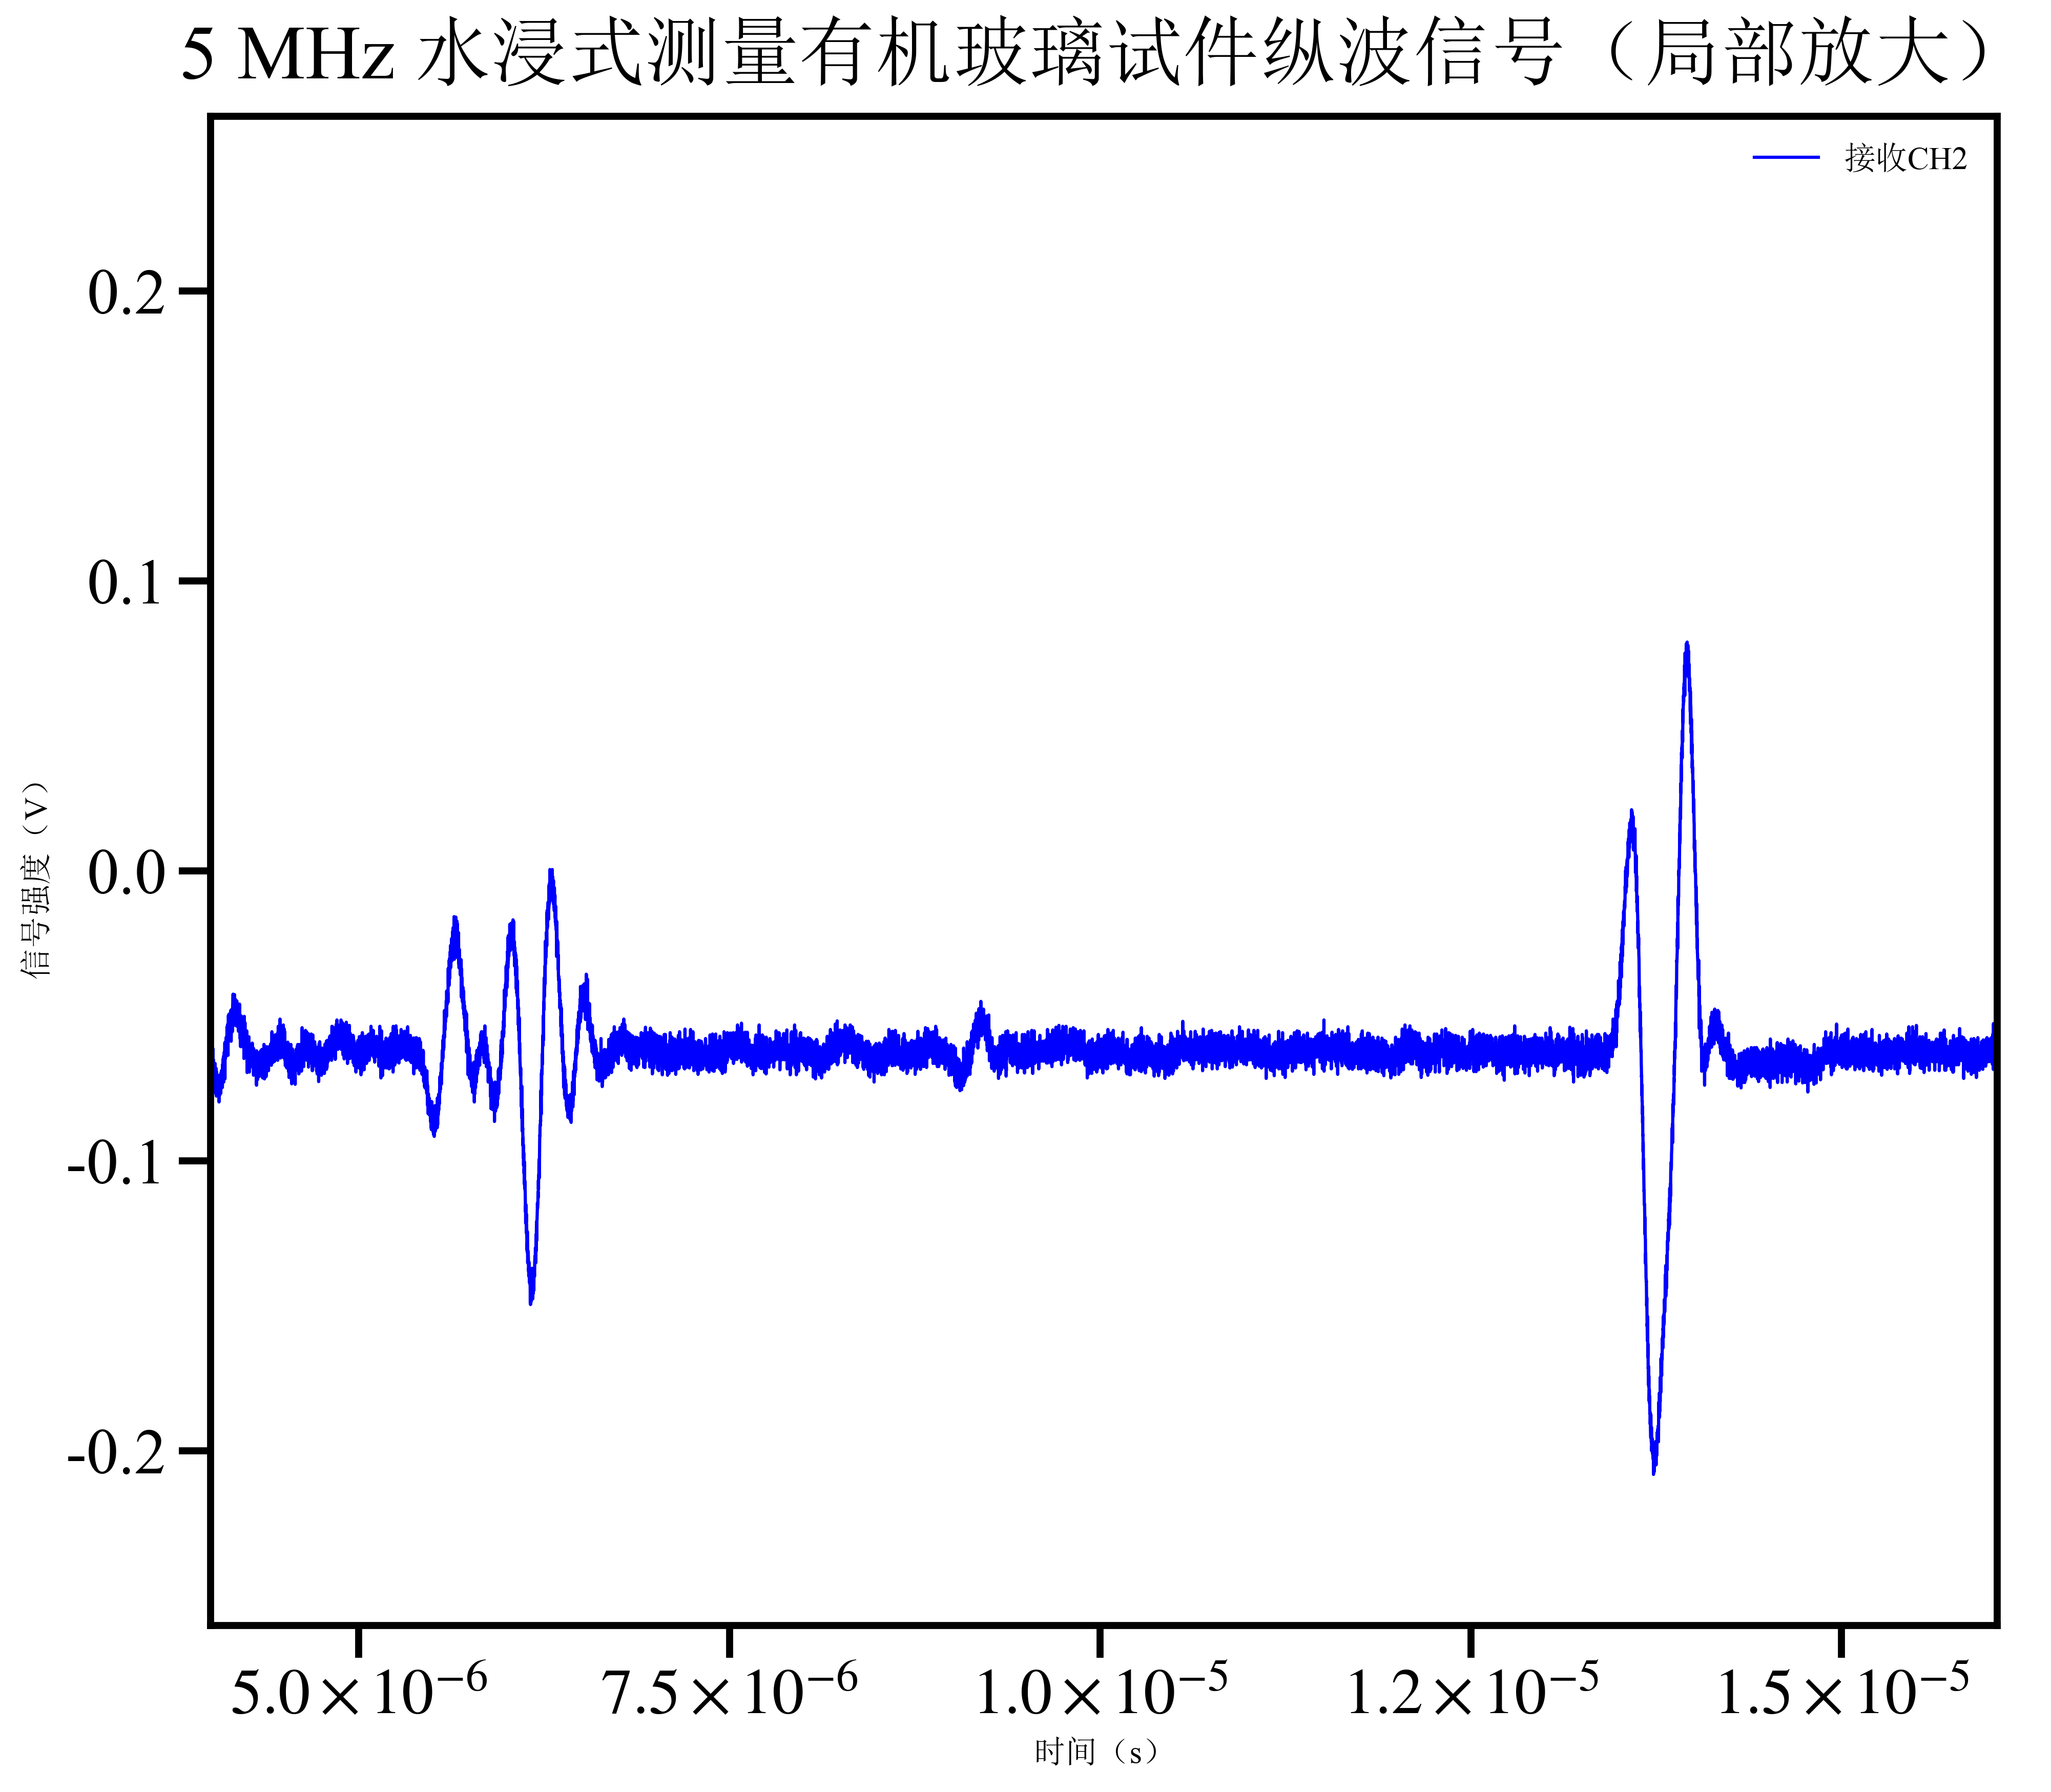
\includegraphics[width=\linewidth]{glass_water_zoom.png}
  （b）输出信号局部放大图
\end{minipage}
\caption{5 MHz 水浸式测量有机玻璃试件纵波波速时信号图}
\label{fig:exp2-og-L}
\end{figure}

\begin{table}[H]
\centering
\caption{5 MHz 水浸式测量三种材料的纵波回波时间差}
\label{tab:exp2-L-time}
\begin{tabular}{lc}
\toprule
材料 & $\Delta t_L$（$\mu$s）\\
\midrule
钢 & 5.05\\
铝 & 4.66\\
有机玻璃 & 7.58\\
\bottomrule
\end{tabular}
\end{table}

由表\ref{tab:exp2-density}的试件厚度和表\ref{tab:exp2-L-time}的时间差计算纵波波速。厚度以 mm、时间差以 $\mu$s 代入时：
\begin{subequations}
\begin{align}
  C_{L,st}&=\frac{2h_{st}}{\Delta t_{L,st}}\times10^3
  =5960\ \mathrm{m/s},\\
  C_{L,al}&=\frac{2h_{al}}{\Delta t_{L,al}}\times10^3
  =6446\ \mathrm{m/s},\\
  C_{L,og}&=\frac{2h_{og}}{\Delta t_{L,og}}\times10^3
  =3720\ \mathrm{m/s}.
\end{align}
\end{subequations}
钢、铝和有机玻璃的纵波波速参考值分别取 $5900$、$6300$ 和 $2730\,\mathrm{m/s}$，对应相对误差为
\begin{subequations}
\begin{align}
  \delta_{L,st}&=\frac{|C_{L,st}-5900|}{5900}\times100\%=1.0\%,\\
  \delta_{L,al}&=\frac{|C_{L,al}-6300|}{6300}\times100\%=2.3\%,\\
  \delta_{L,og}&=\frac{|C_{L,og}-2730|}{2730}\times100\%=36.3\%.
\end{align}
\end{subequations}
结合信号强度、材料非均匀性和波峰位置的选取分析偏差。本组钢、铝结果与参考值吻合较好；有机玻璃水浸信号回波成分复杂，除上下表面回波外混有水面与盆底反射杂波，所识别回波间隔对应的波速与参考值偏差较大，仅供参考（有机玻璃纵波波速以接触式测量为准）。
本组钢、铝试件纵波波速分别为 $5960\,\mathrm{m/s}$ 和 $6446\,\mathrm{m/s}$，与参考值偏差仅 $1.0\%$ 和 $2.3\%$；两者回波列规则、相邻回波间隔稳定，读数可靠。有机玻璃信号回波成分复杂，波峰归属难以确定，故其水浸波速仅供参考，以接触式测量结果为准。

\subsection{水浸式测量三种材料的衰减系数}
利用同一次波形中试件上下表面的不同反射回波，读取第 $m$、$n$ 个回波的幅值 $P_m$、$P_n$（$n>m$），再按式\eqref{eq:exp2-attenuation}计算衰减系数。计算时将表\ref{tab:exp2-density}中的试件厚度由 mm 换算为 cm，结果填入表\ref{tab:exp2-attenuation}。

\begin{table}[H]
\centering
\caption{5 MHz 水浸式测量三种材料的纵波衰减系数}
\label{tab:exp2-attenuation}
\begin{tabular}{lccc}
\toprule
材料 & $P_m$（V），回波序号 $m$ & $P_n$（V），回波序号 $n$ & $\alpha_L$（dB/cm）\\
\midrule
钢 & 0.401，$m=1$ & 0.142，$n=2$ & 3.00\\
铝 & 0.655，$m=1$ & 0.325，$n=2$ & 2.03\\
有机玻璃 & 0.208，$m=1$ & 0.073，$n=2$ & 3.23\\
\bottomrule
\end{tabular}
\end{table}

比较三种材料的衰减程度，并分析后续回波信号较弱时波峰读取对结果的影响。注意本组有机玻璃水浸信号的第二回波幅值已接近噪声水平，其衰减系数仅供参考。
三种材料的纵波衰减系数分别为钢 $3.00\,\mathrm{dB/cm}$、铝 $2.03\,\mathrm{dB/cm}$、有机玻璃 $3.23\,\mathrm{dB/cm}$。水浸测量中回波幅值包含水--试件界面的透射损失，衰减系数较材料真实值偏大，但材料间的相对比较仍有意义；后续回波越弱，波峰读取对结果的影响越显著。

\subsection{接触式测量三种材料的横波波速}
使用频率为 5 MHz 的横波超声探头进行接触式测量。本组增益设置为：钢、铝试件 10 dB，有机玻璃试件 30 dB。波形数据及用于计算波速的数据区域如图\ref{fig:exp2-steel-S}--图\ref{fig:exp2-og-S}所示，波峰时间差填入表\ref{tab:exp2-S-time}。

\begin{figure}[H]
\centering
\begin{minipage}[t]{0.48\textwidth}
  \centering
  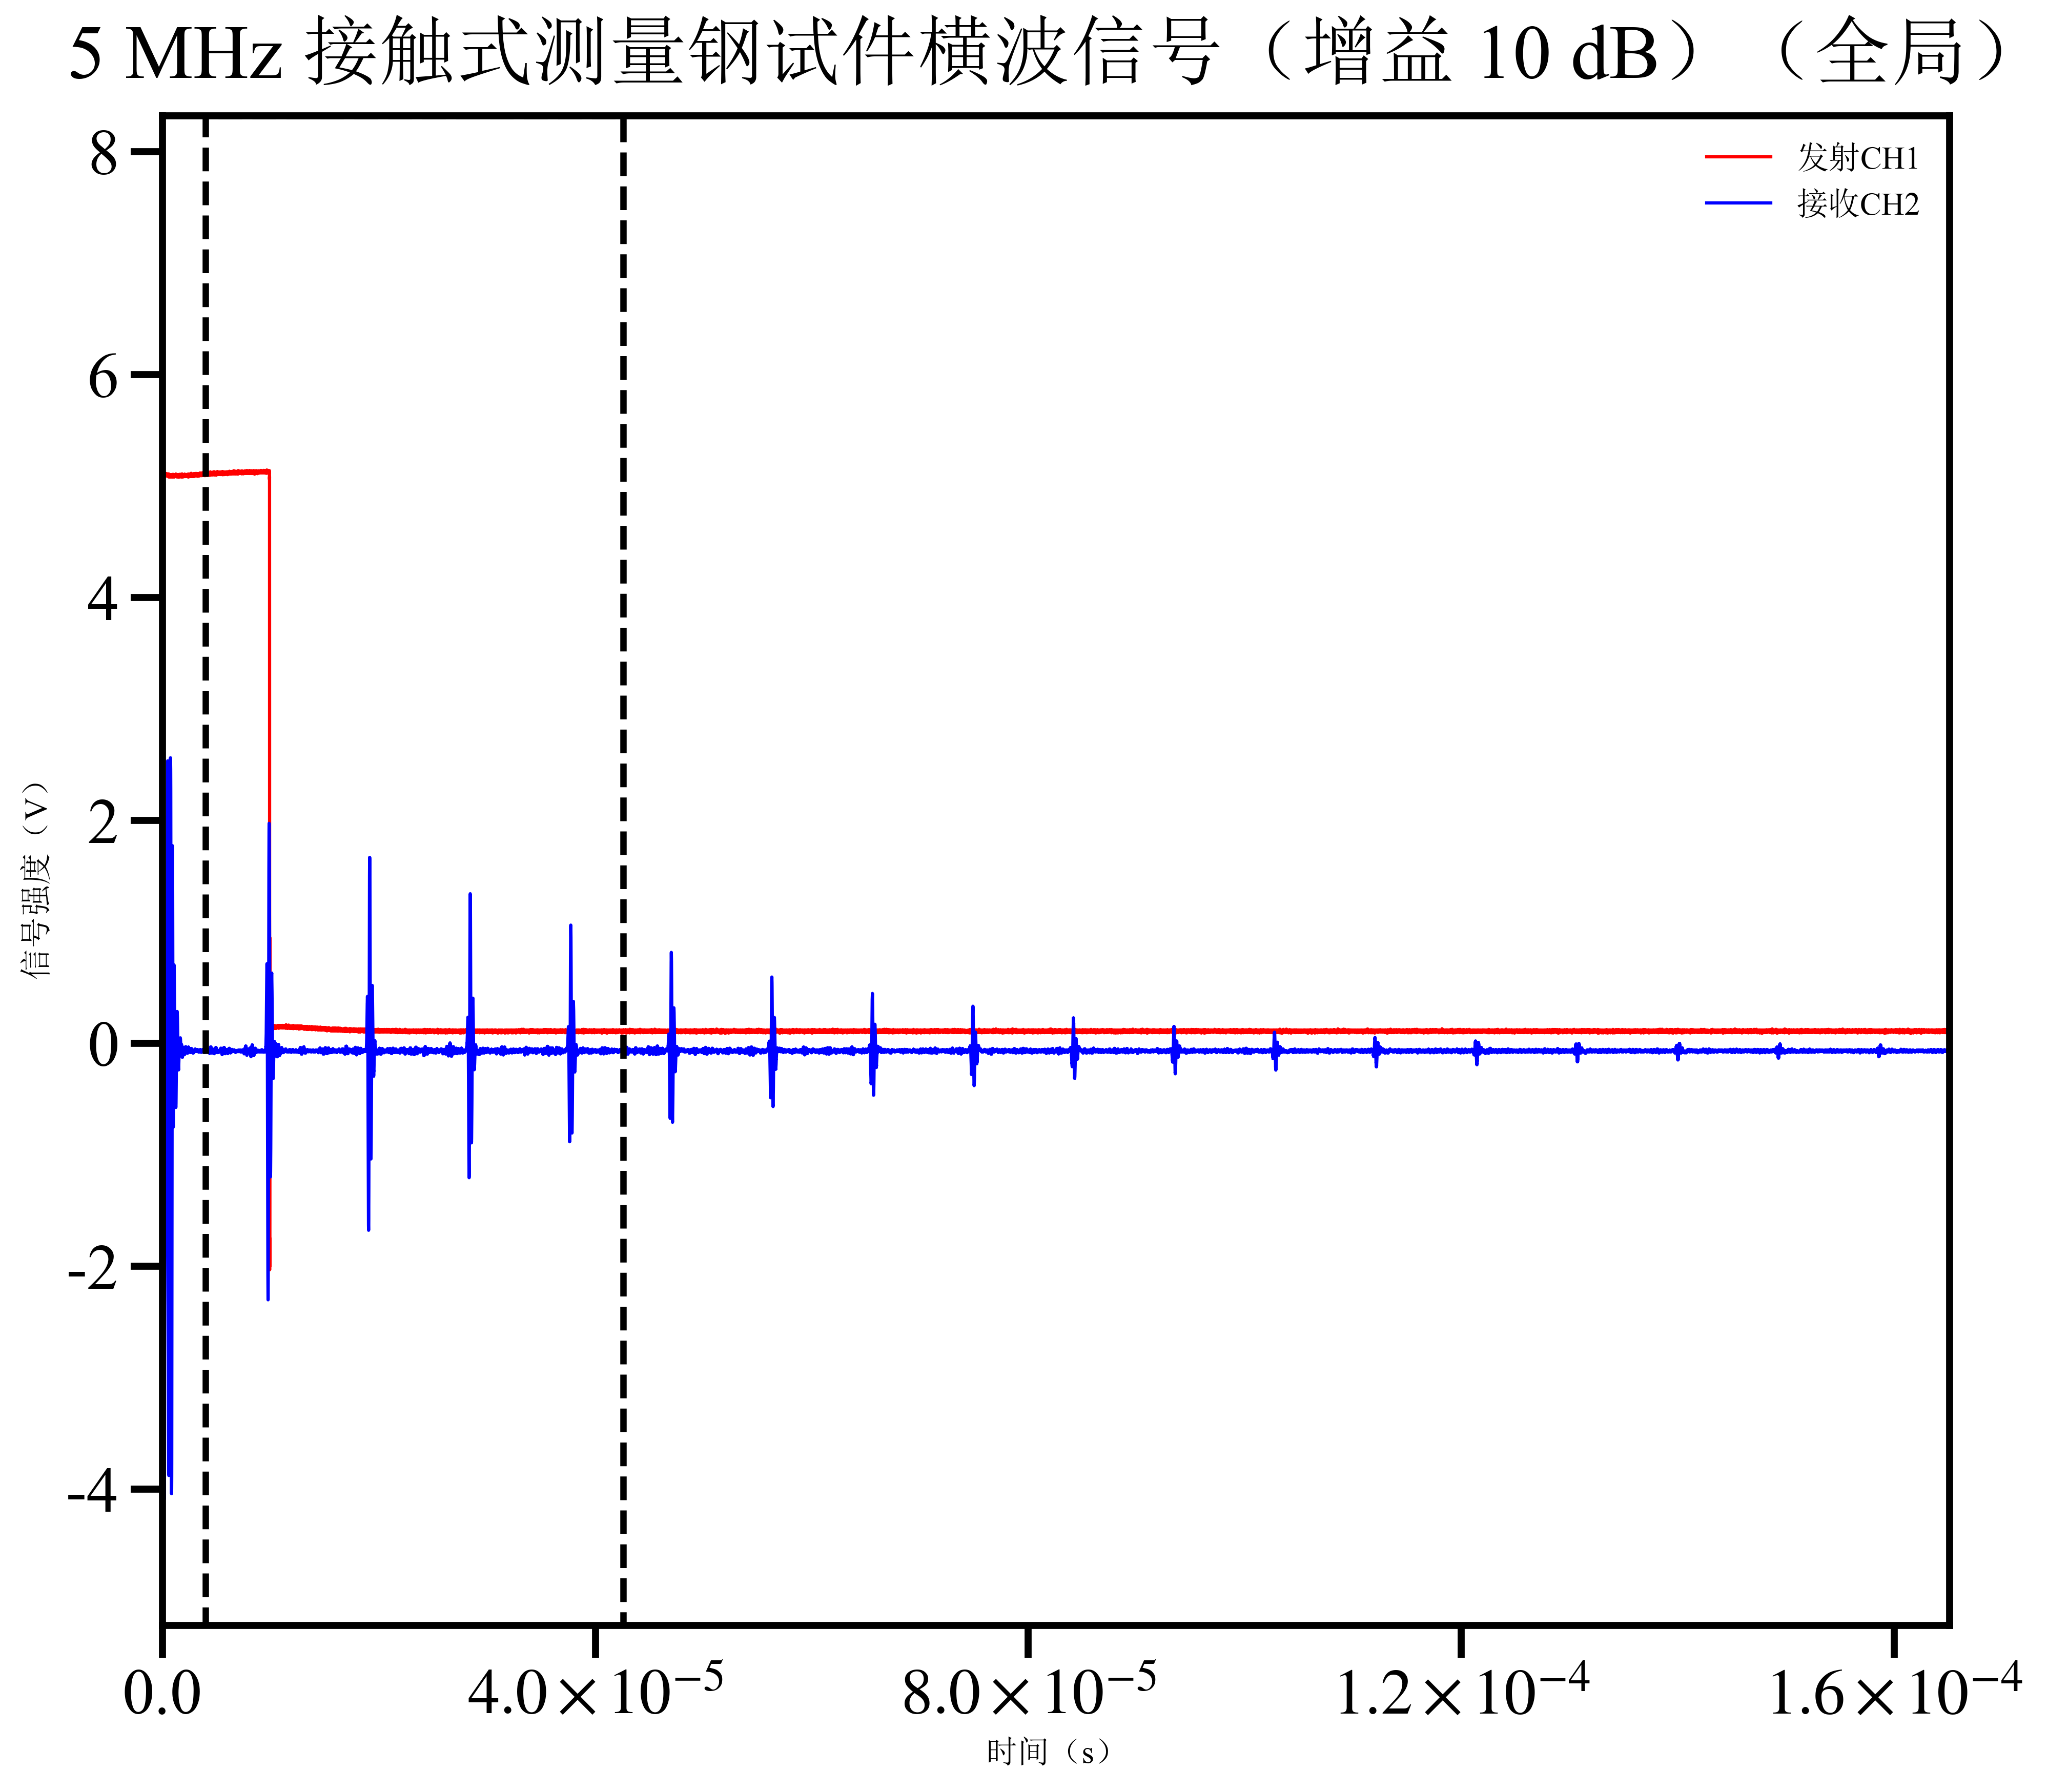
\includegraphics[width=\linewidth]{steel_5S_global.png}
  （a）输入输出信号全局图
\end{minipage}\hfill
\begin{minipage}[t]{0.48\textwidth}
  \centering
  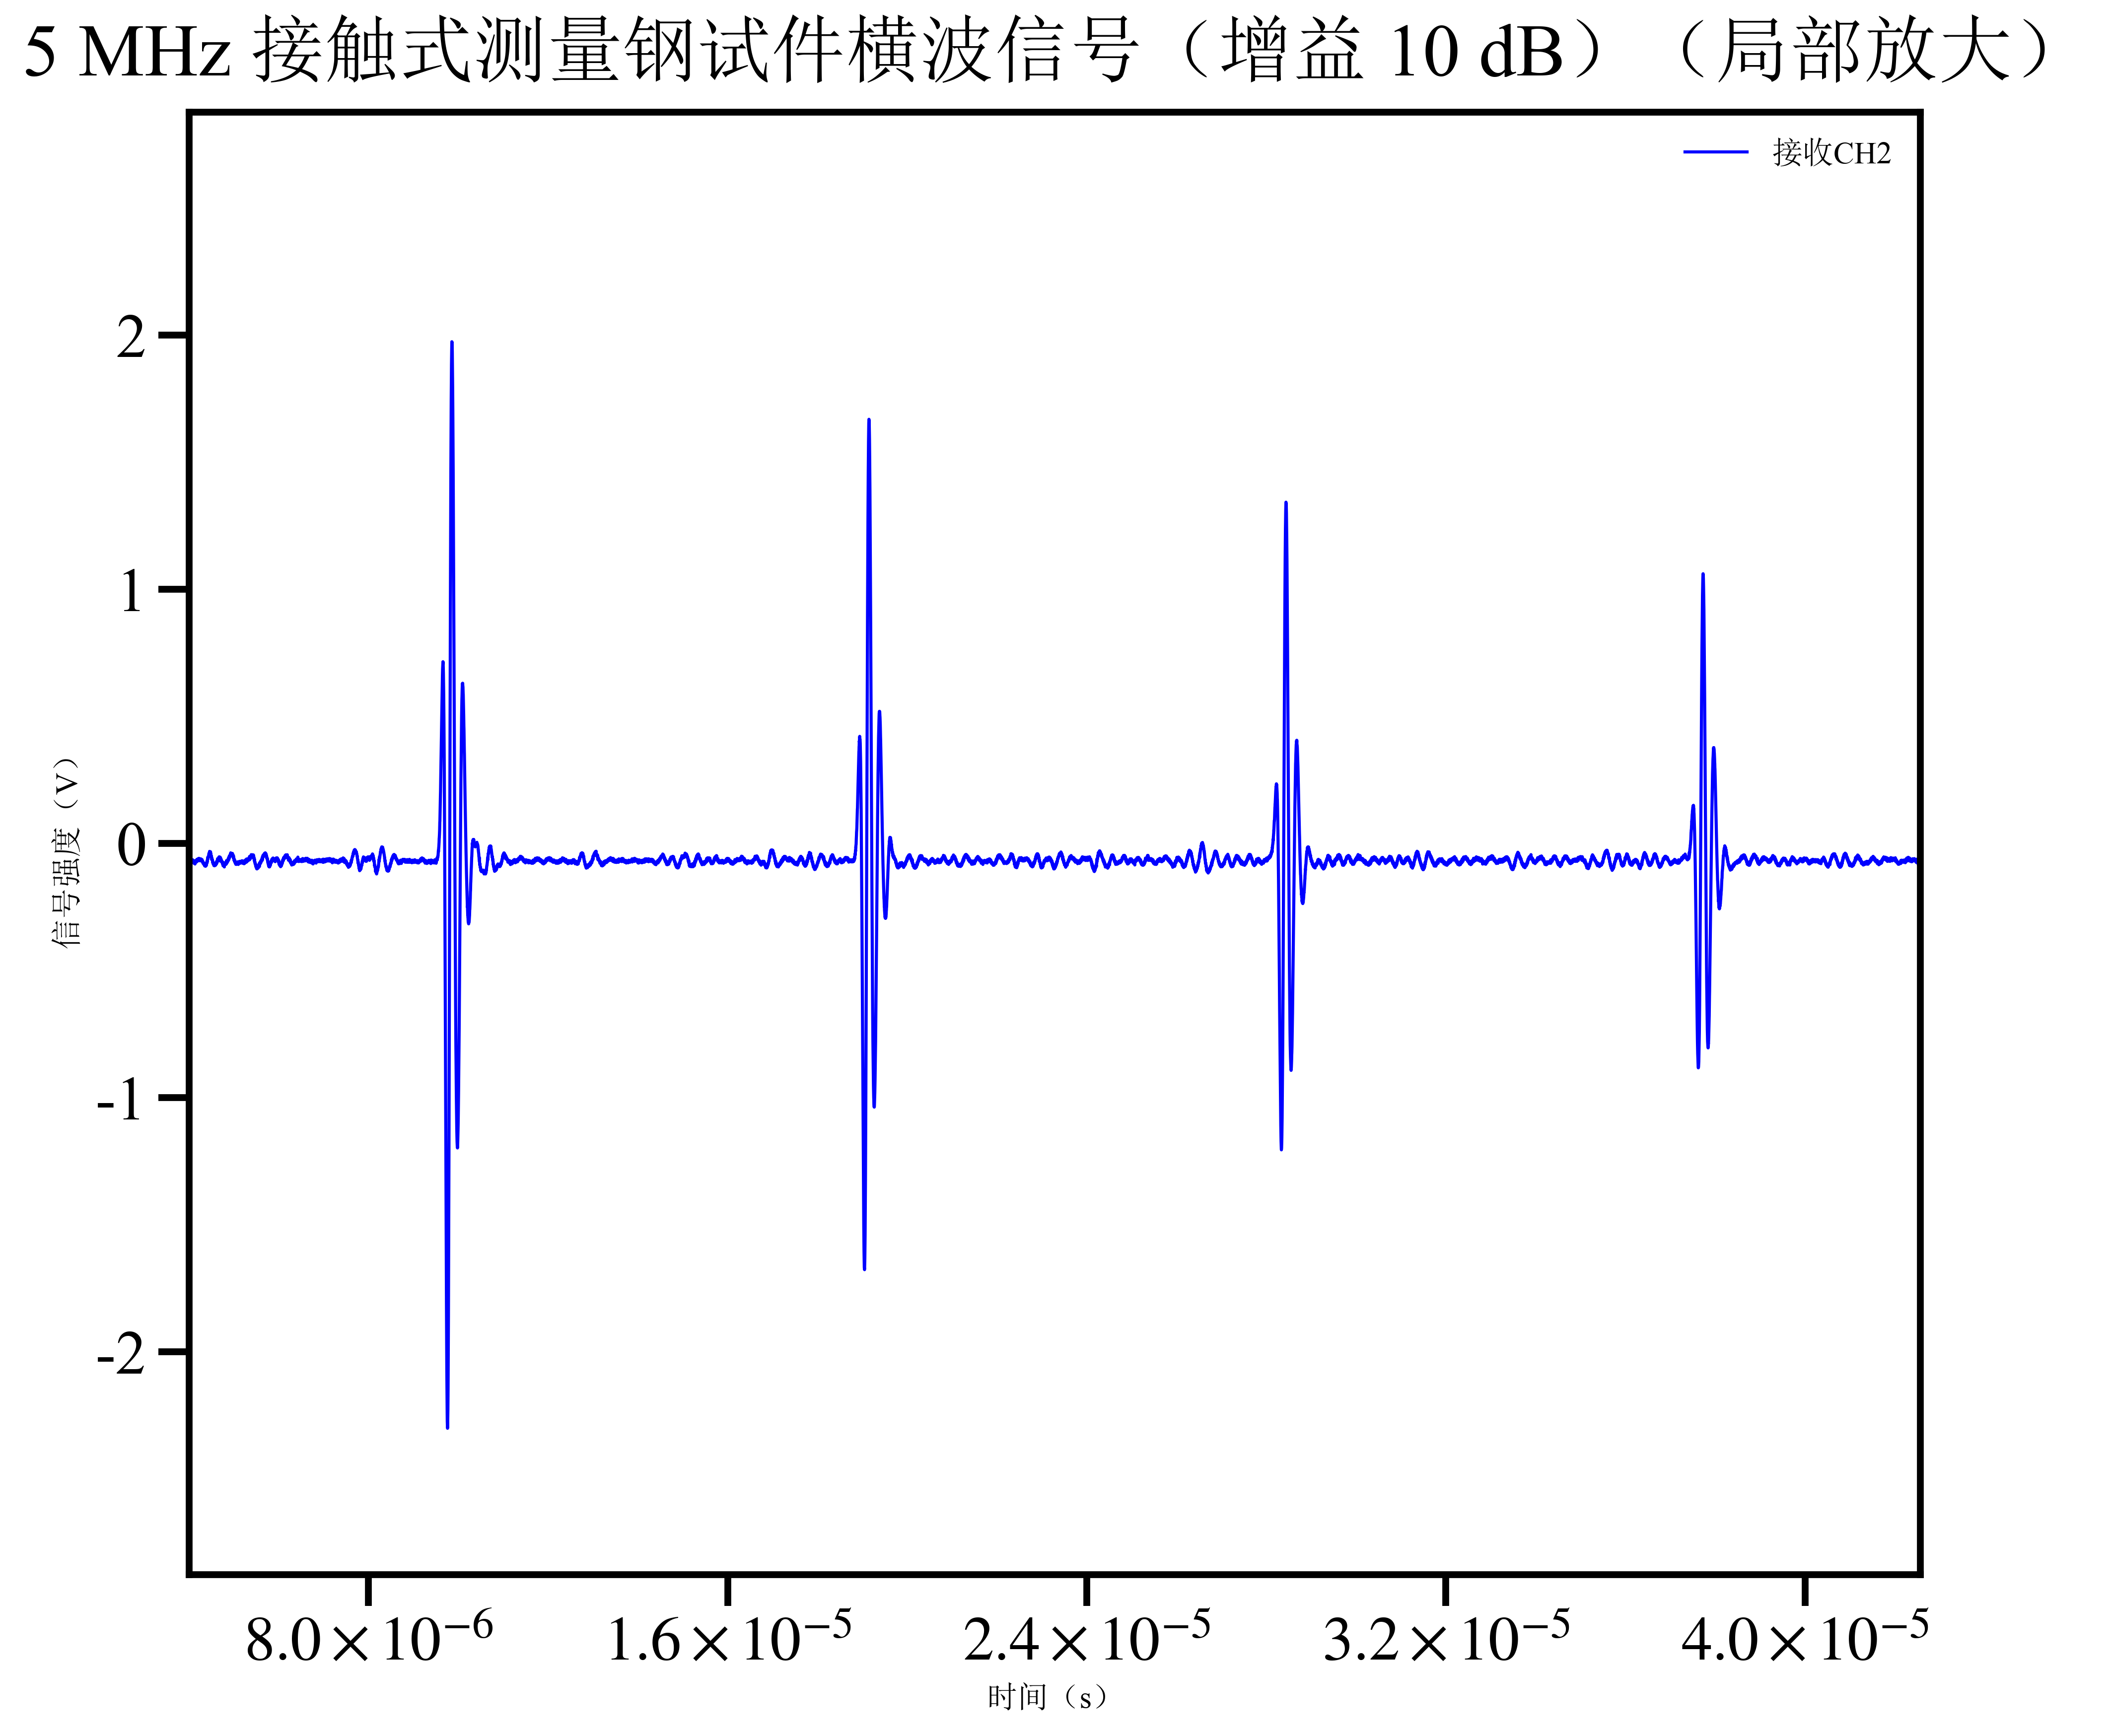
\includegraphics[width=\linewidth]{steel_5S_zoom.png}
  （b）输出信号局部放大图
\end{minipage}
\caption{5 MHz 接触式测量钢试件横波波速时信号图}
\label{fig:exp2-steel-S}
\end{figure}

\begin{figure}[H]
\centering
\begin{minipage}[t]{0.48\textwidth}
  \centering
  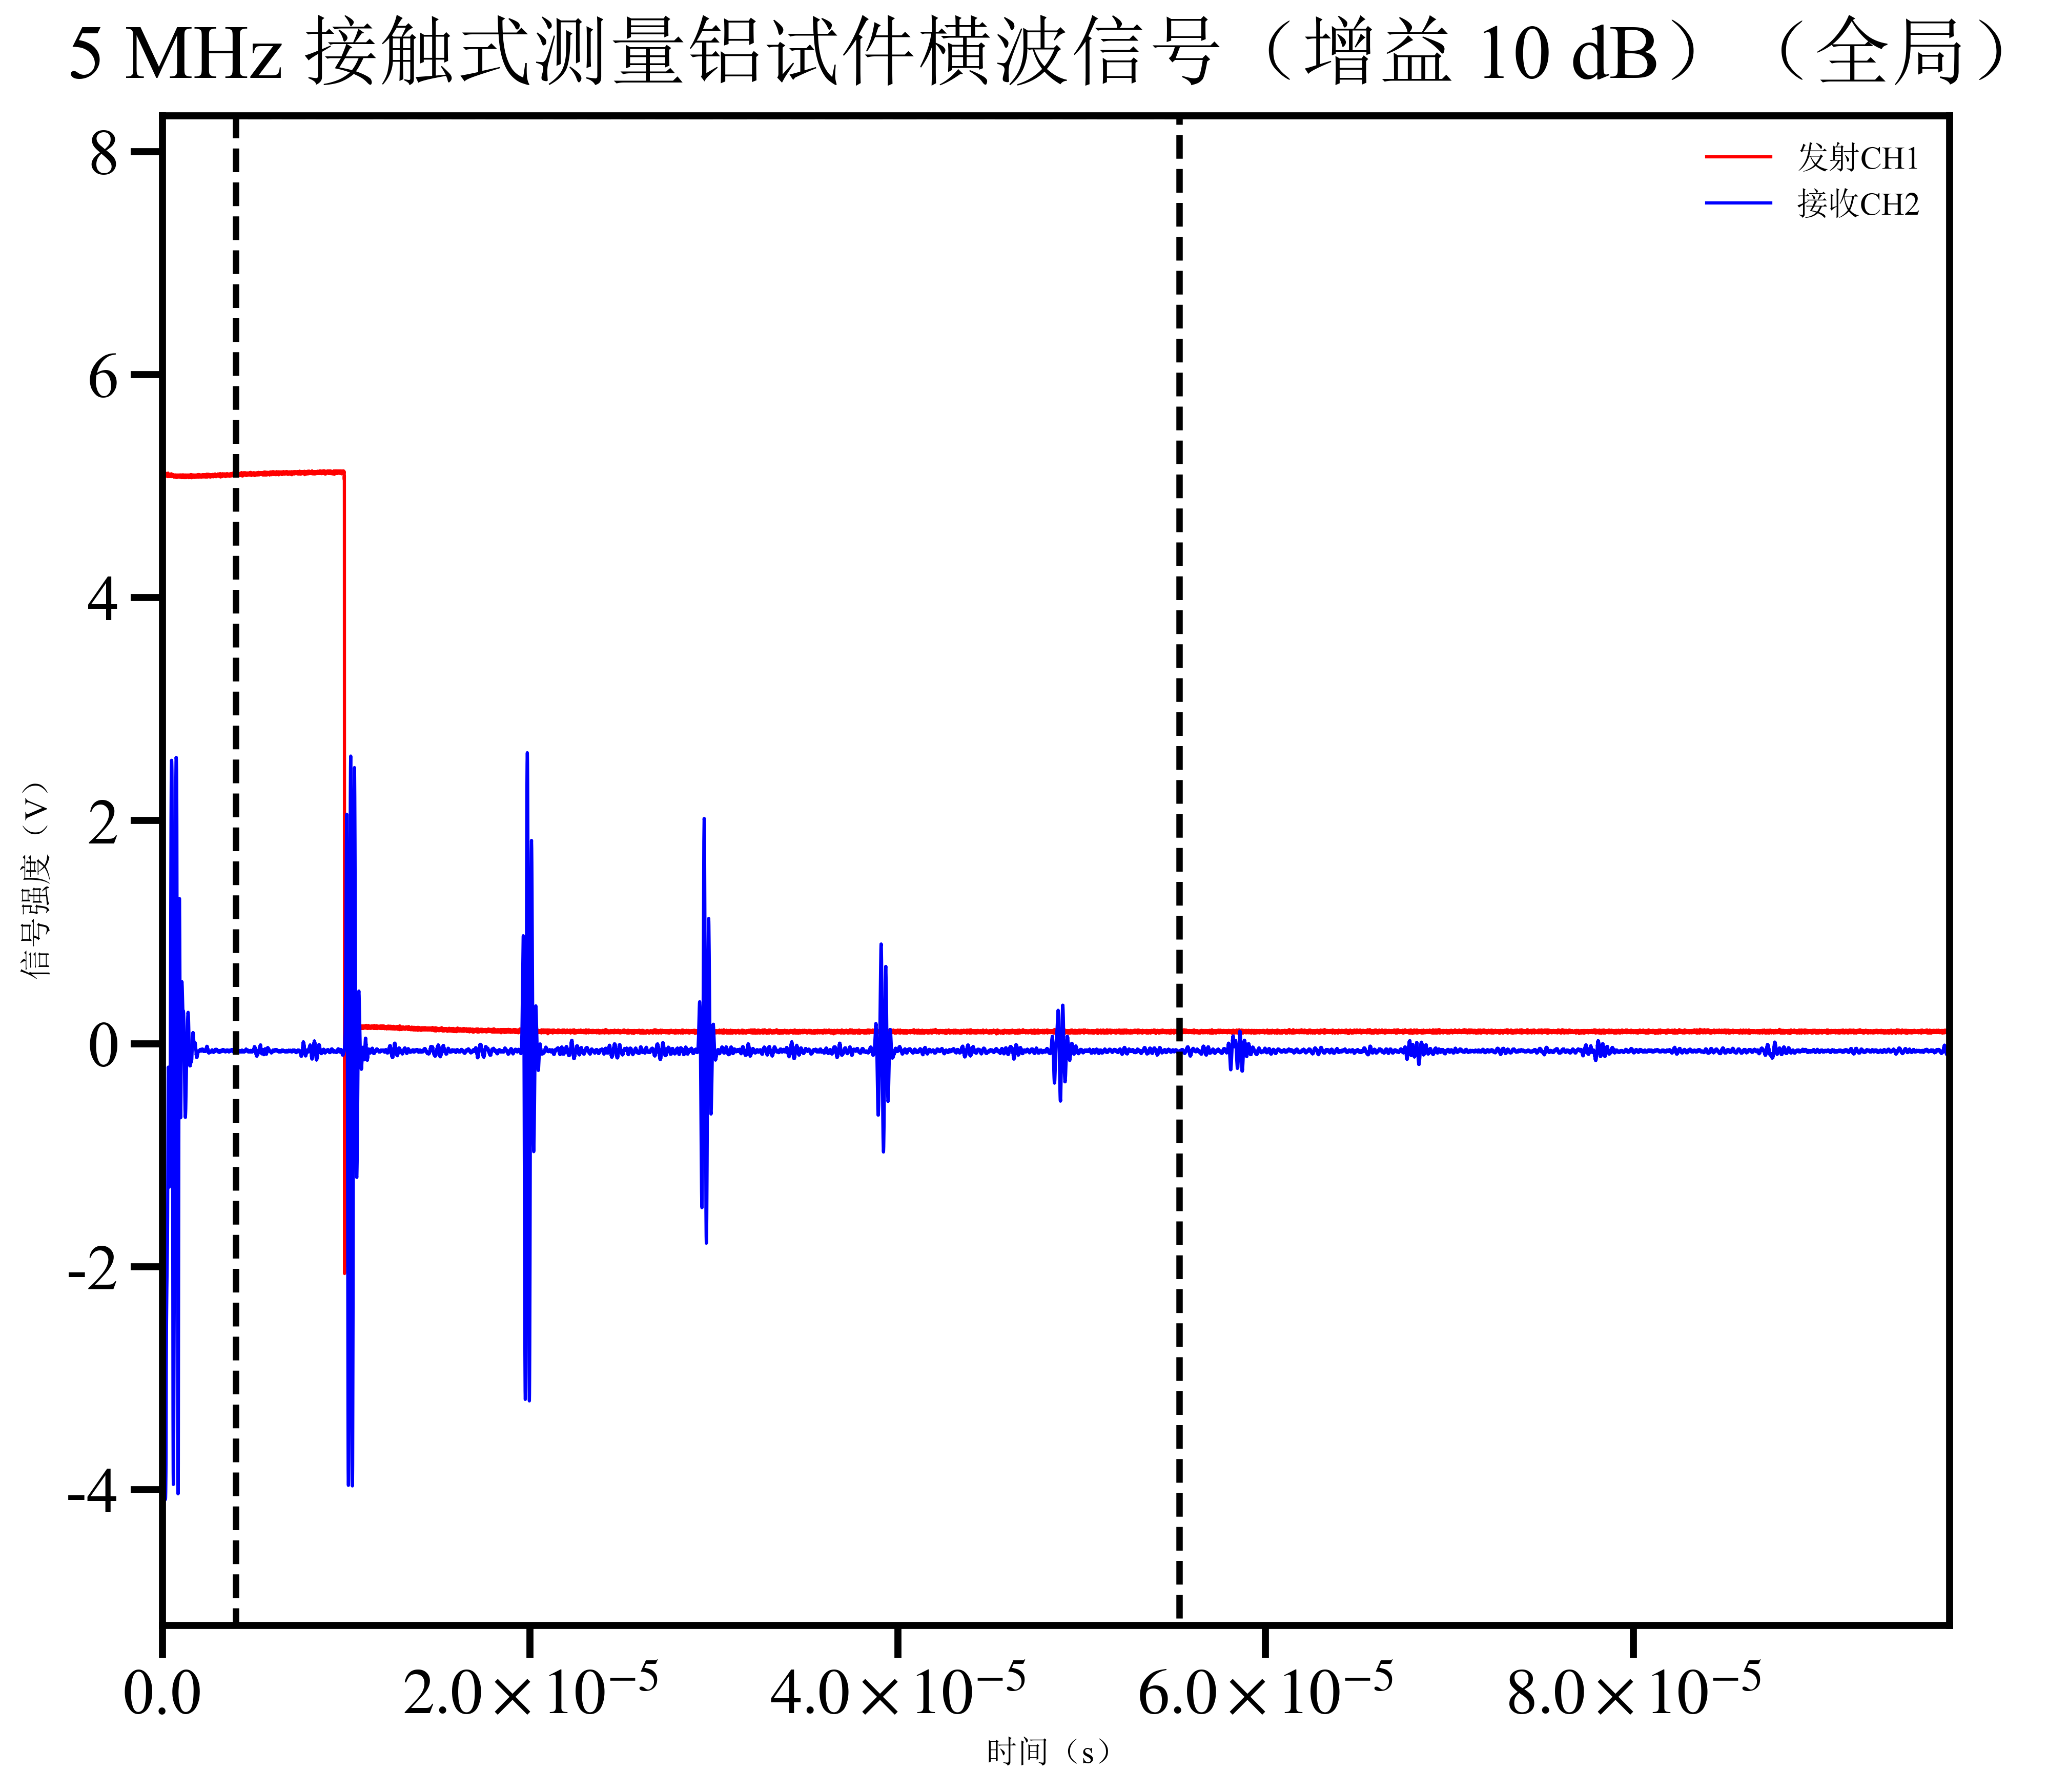
\includegraphics[width=\linewidth]{alu_5S_global.png}
  （a）输入输出信号全局图
\end{minipage}\hfill
\begin{minipage}[t]{0.48\textwidth}
  \centering
  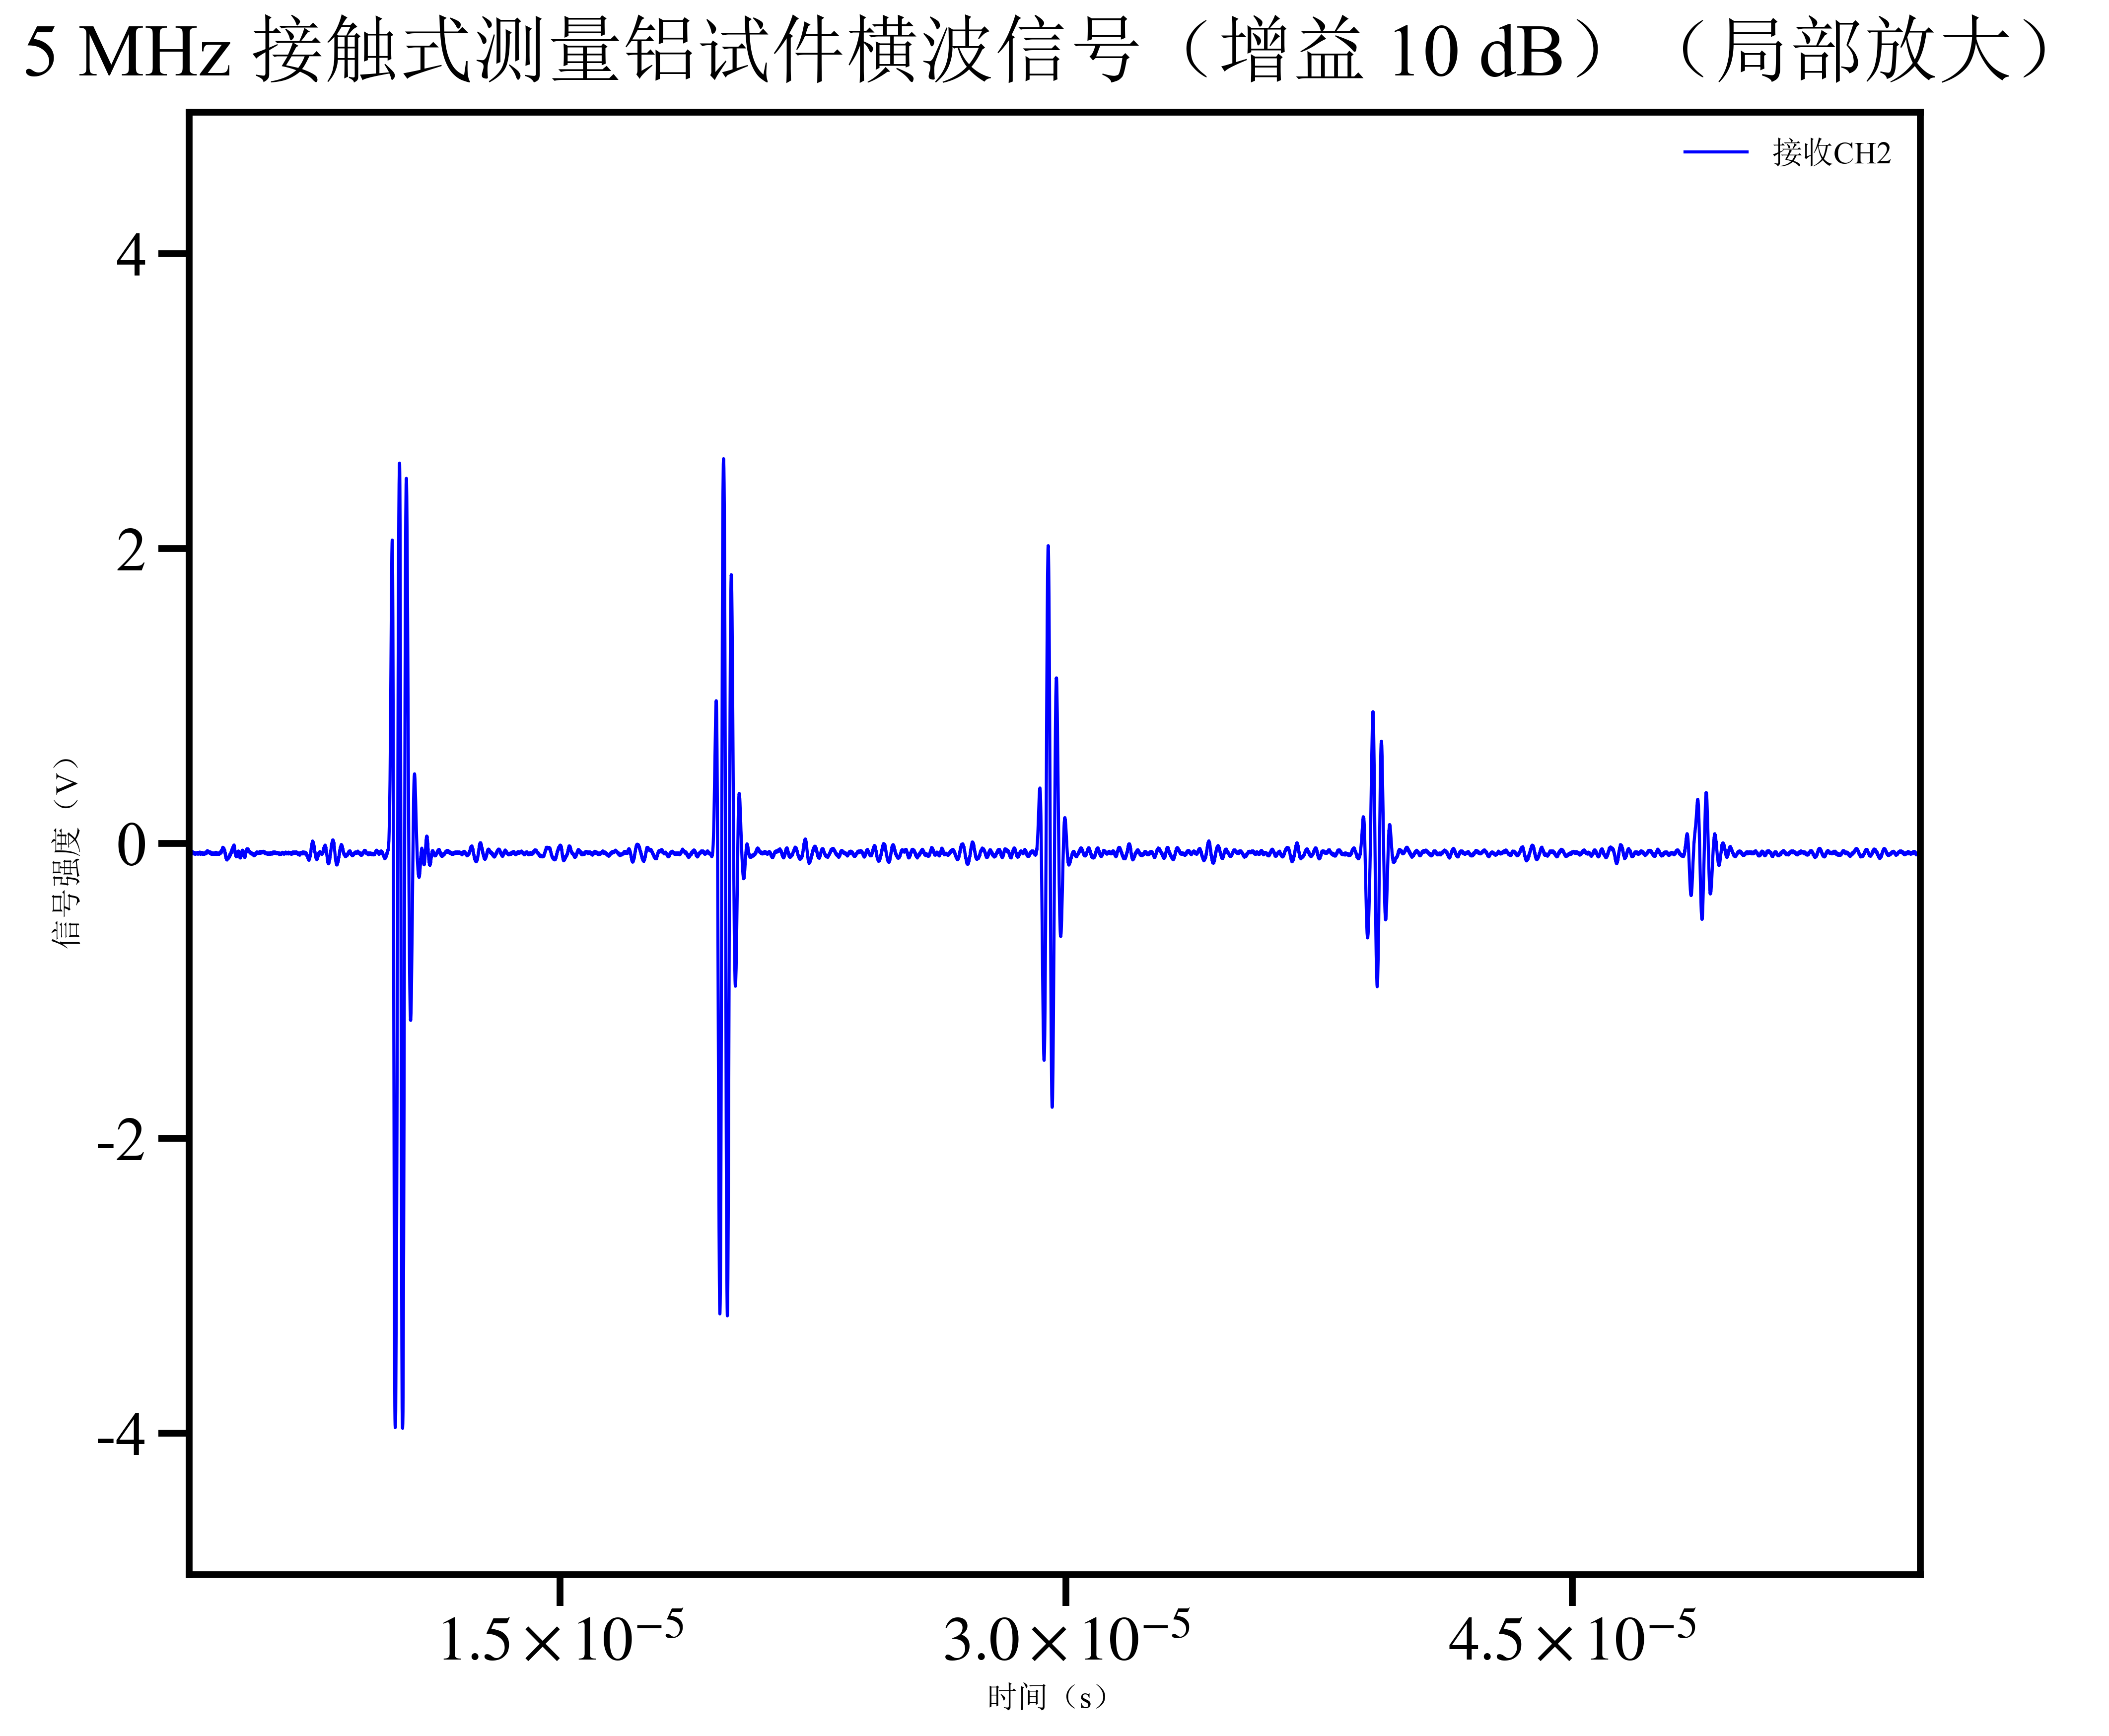
\includegraphics[width=\linewidth]{alu_5S_zoom.png}
  （b）输出信号局部放大图
\end{minipage}
\caption{5 MHz 接触式测量铝试件横波波速时信号图}
\end{figure}

\begin{figure}[H]
\centering
\begin{minipage}[t]{0.48\textwidth}
  \centering
  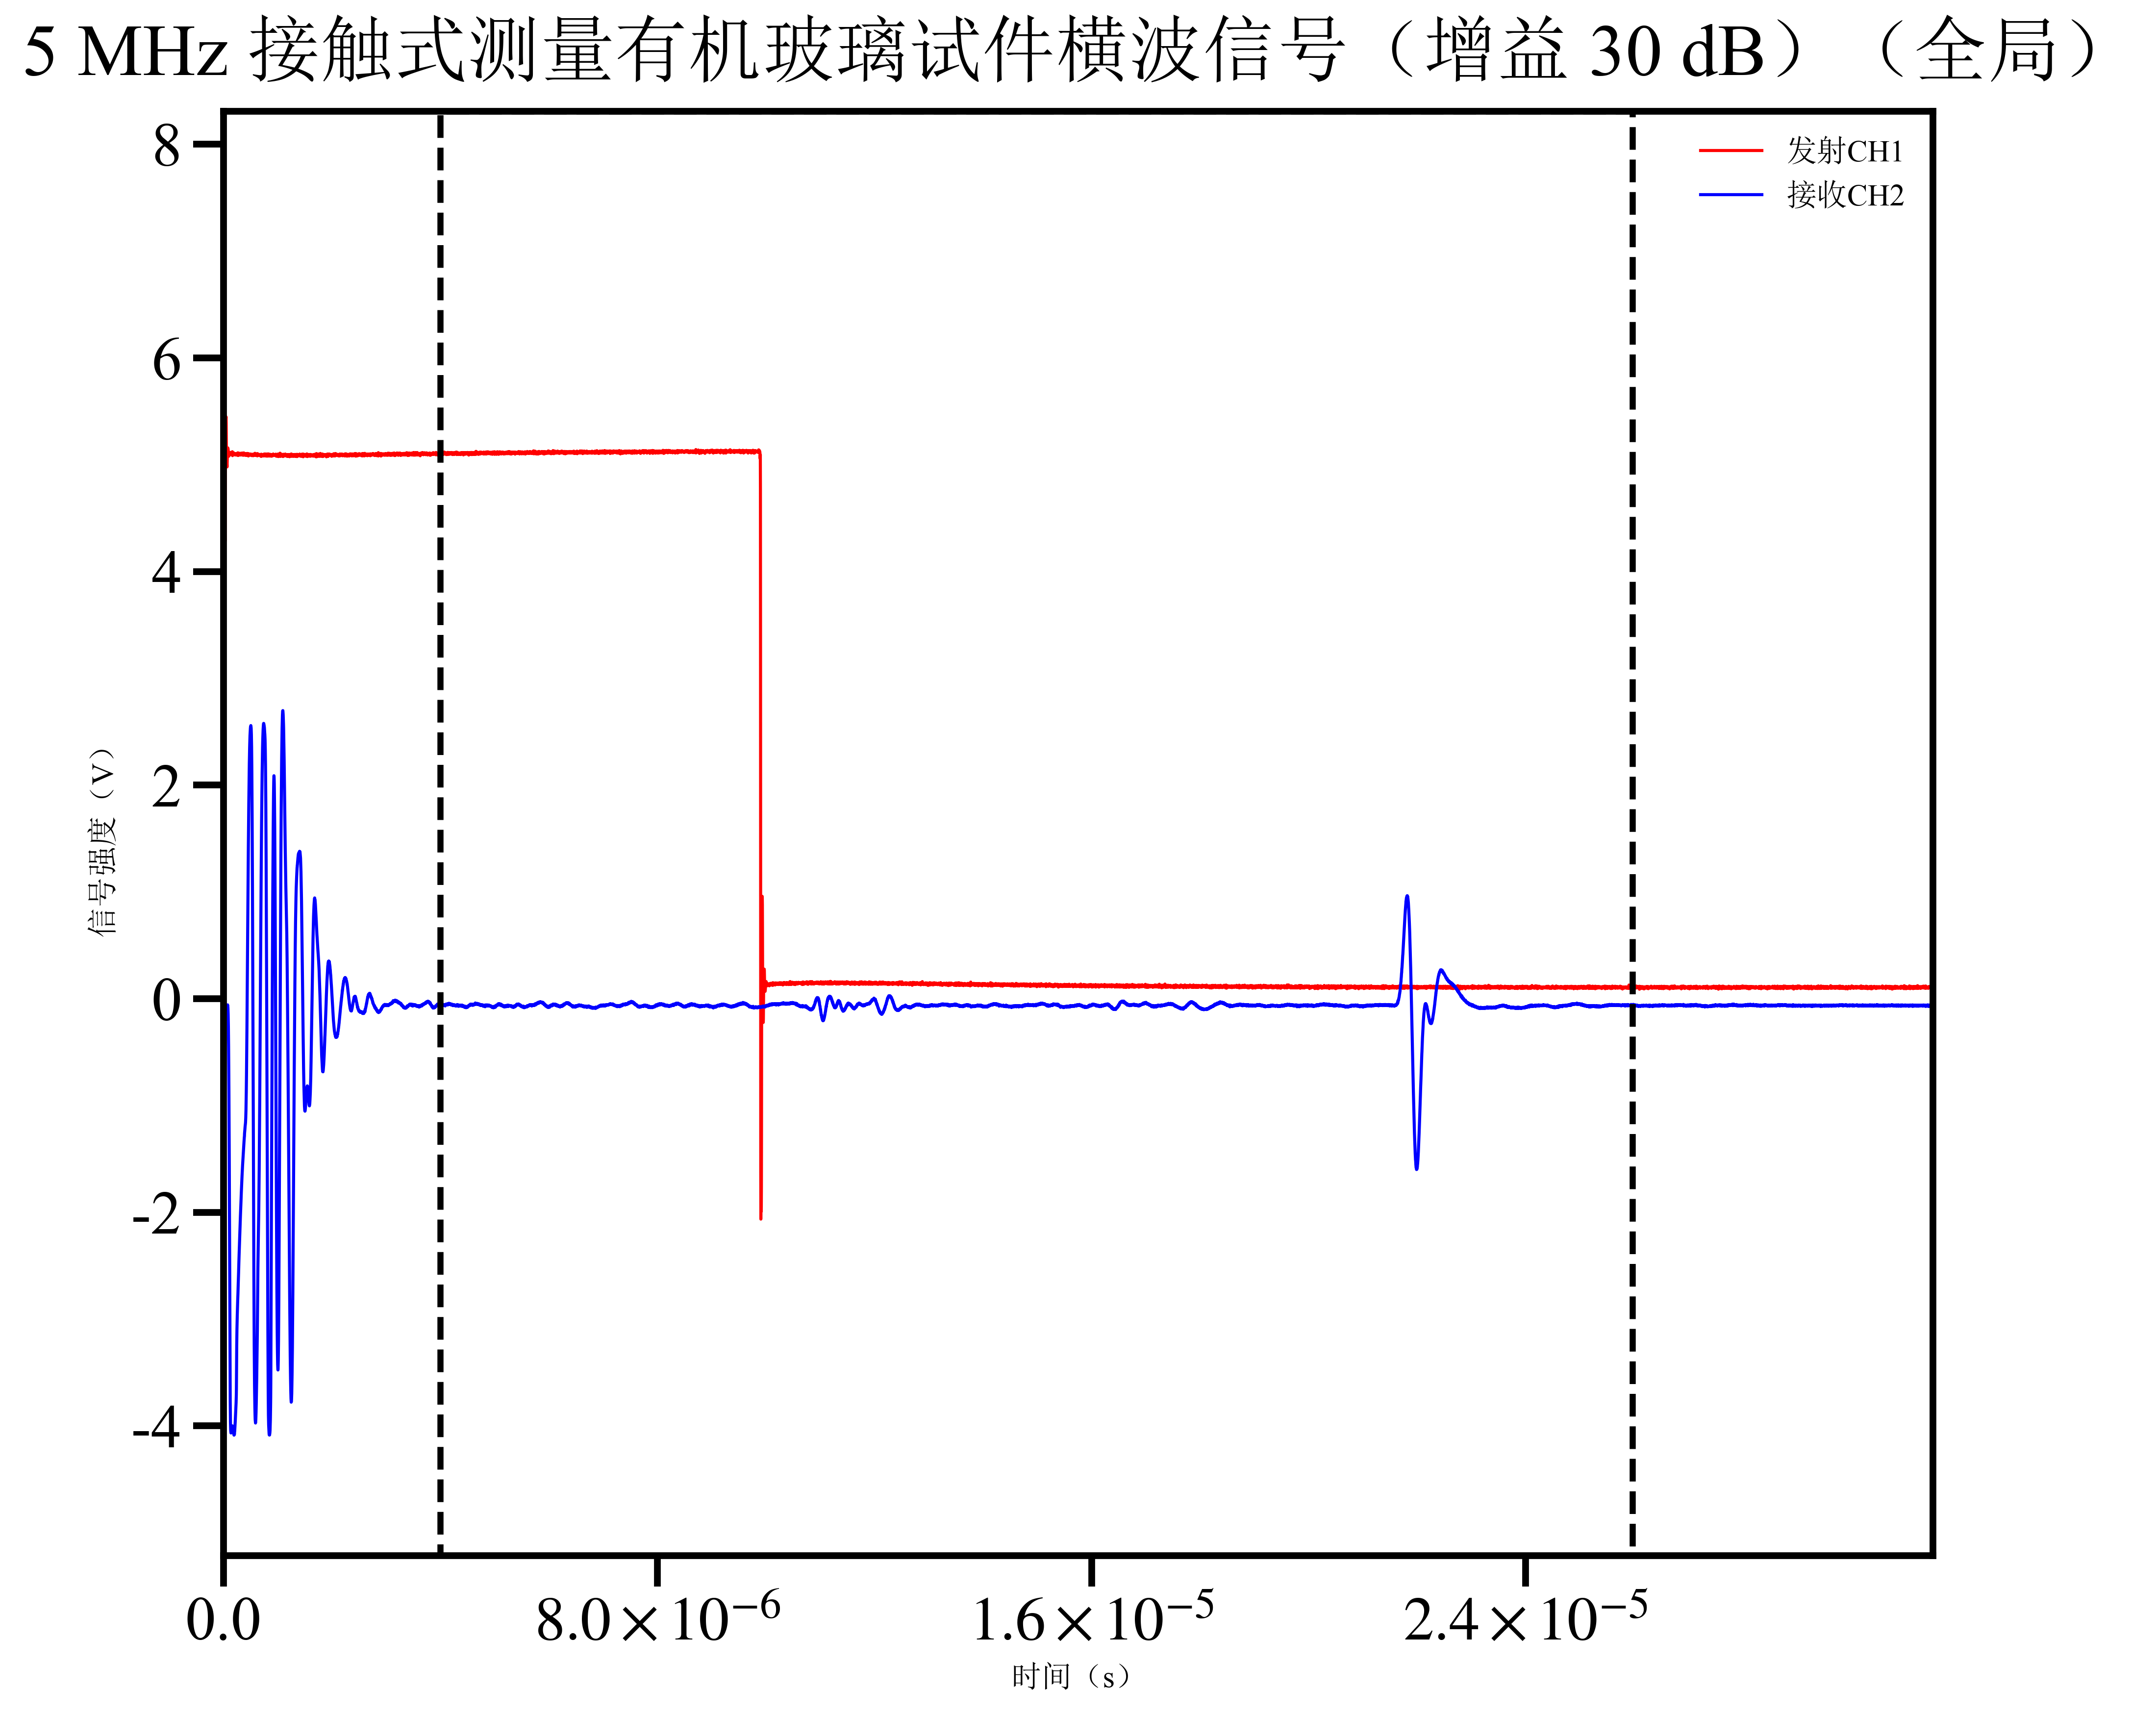
\includegraphics[width=\linewidth]{glass_5S_global.png}
  （a）输入输出信号全局图
\end{minipage}\hfill
\begin{minipage}[t]{0.48\textwidth}
  \centering
  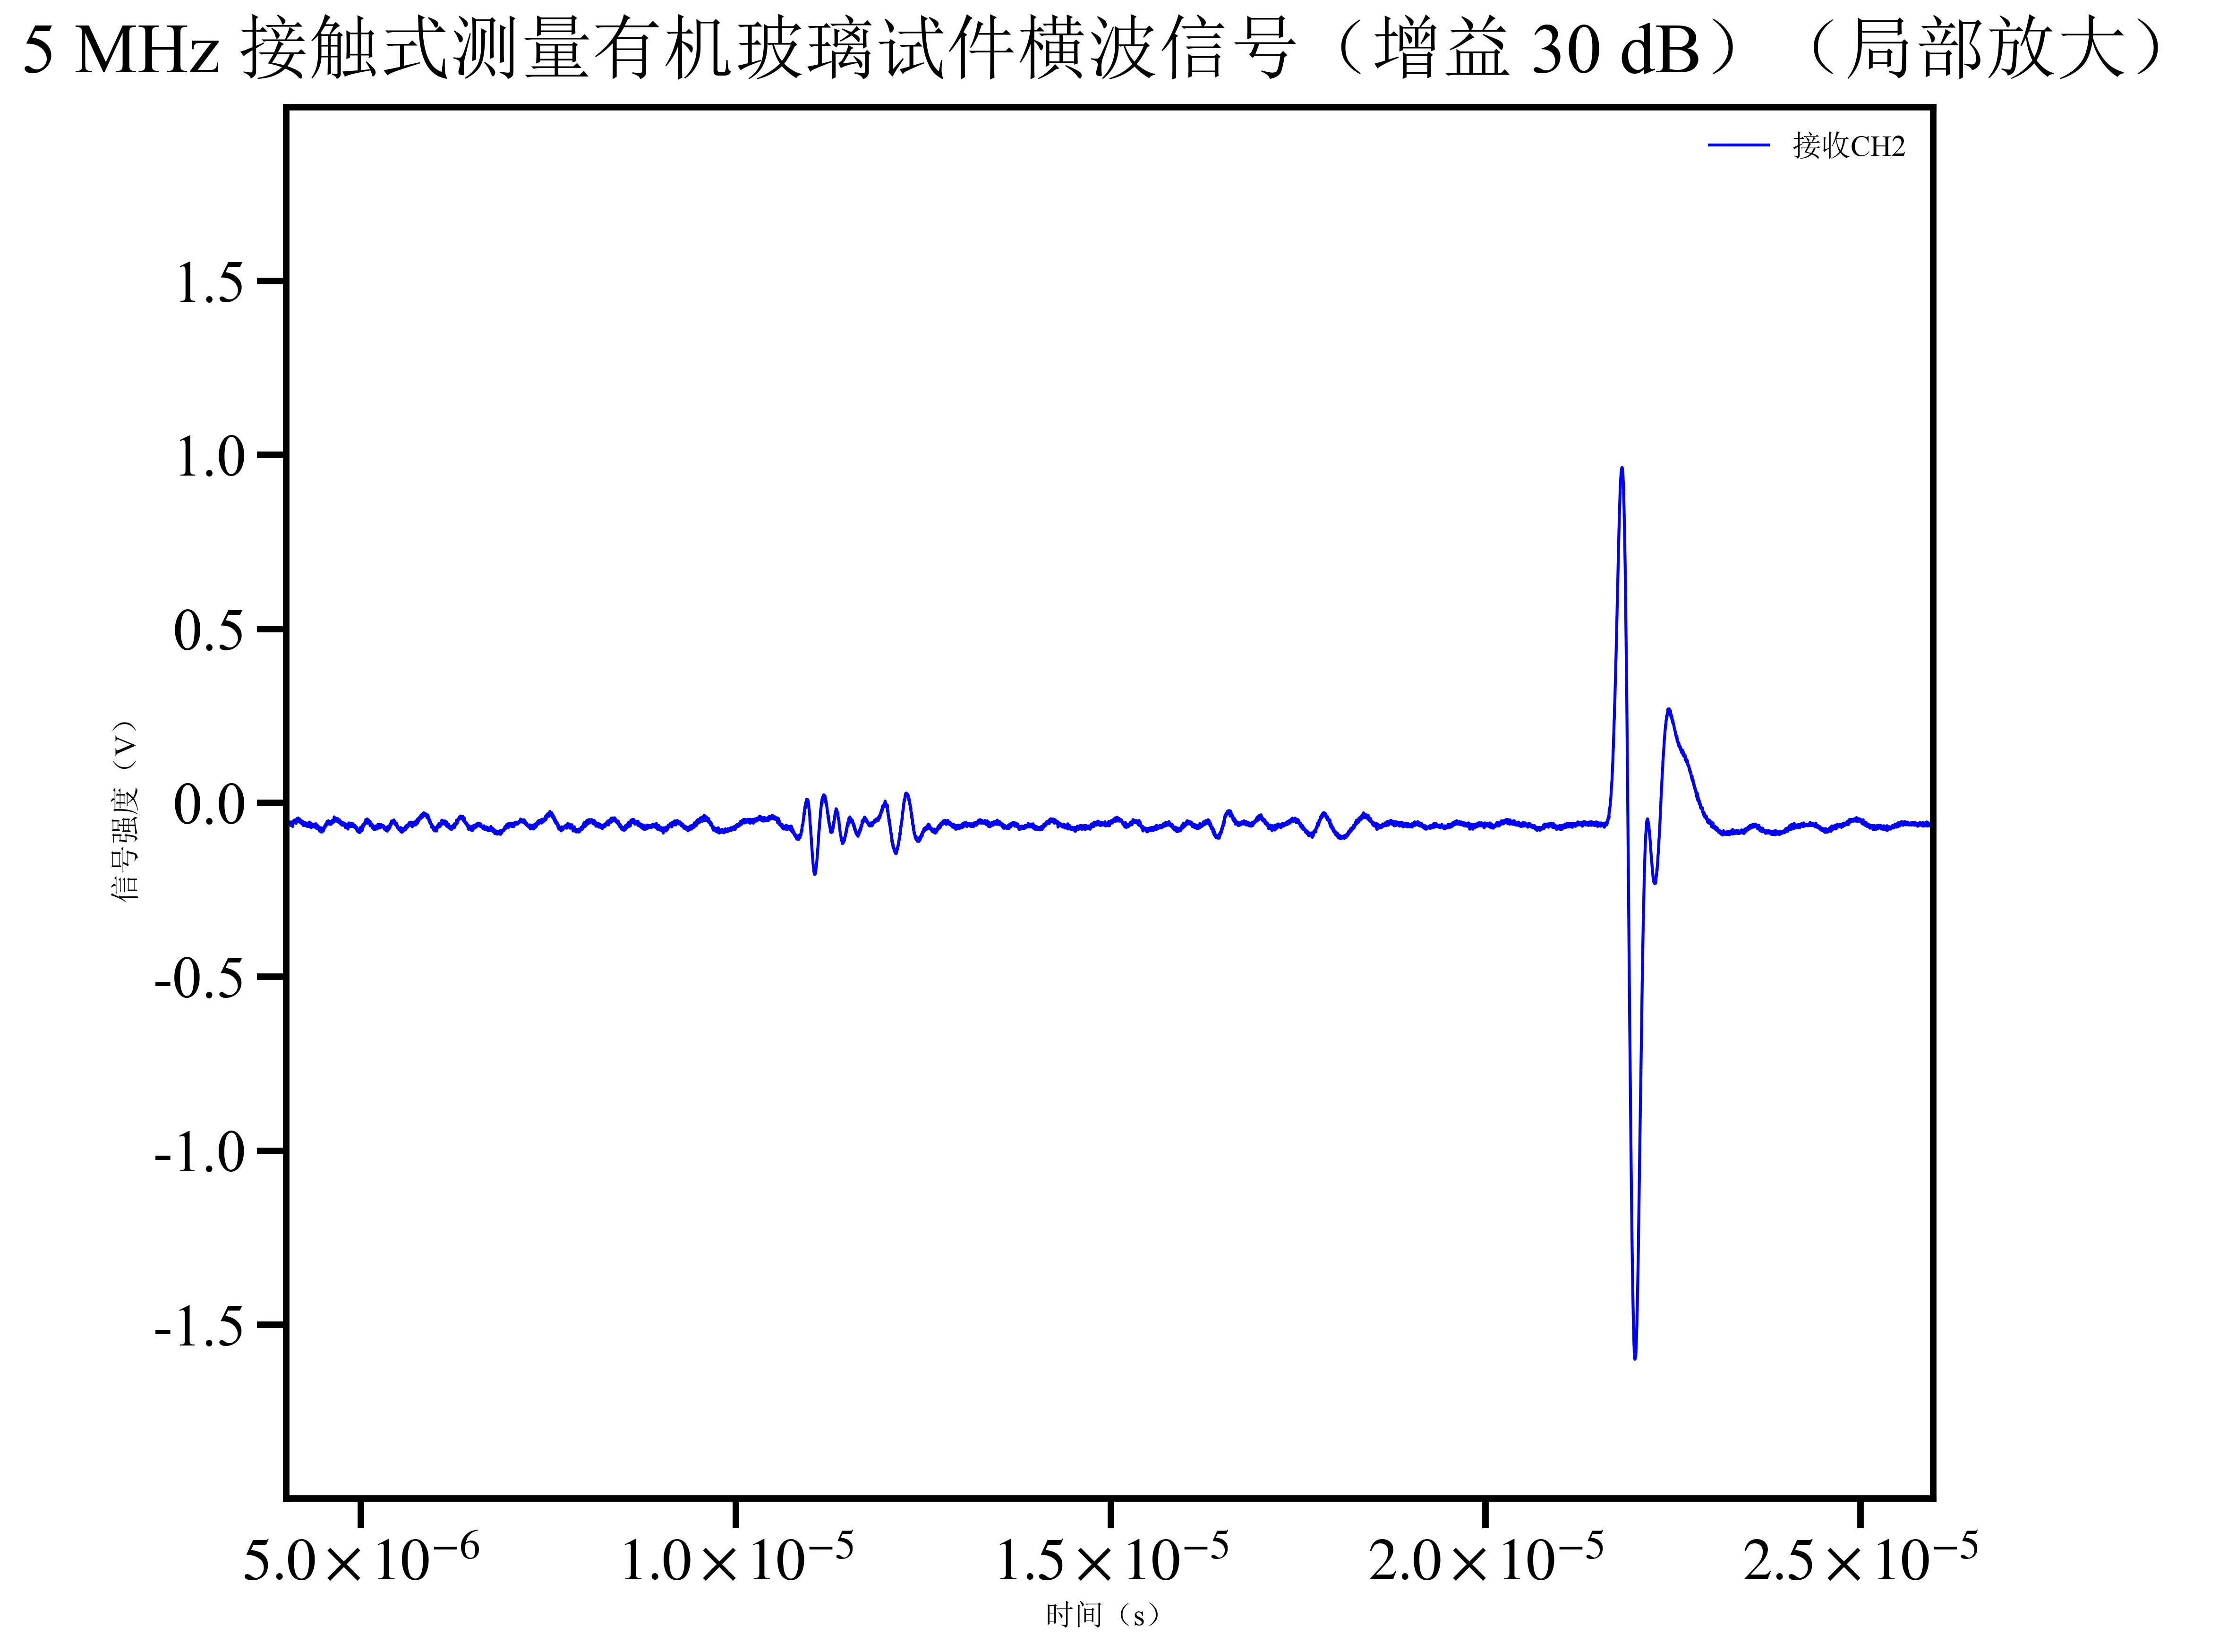
\includegraphics[width=\linewidth]{glass_5S_zoom.png}
  （b）输出信号局部放大图
\end{minipage}
\caption{5 MHz 接触式测量有机玻璃试件横波波速时信号图}
\label{fig:exp2-og-S}
\end{figure}

\begin{table}[H]
\centering
\caption{5 MHz 接触式测量三种材料的横波回波时间差}
\label{tab:exp2-S-time}
\begin{tabular}{lc}
\toprule
材料 & $\Delta t_S$（$\mu$s）\\
\midrule
钢 & 9.29\\
铝 & 9.63\\
有机玻璃 & 21.99\\
\bottomrule
\end{tabular}
\end{table}

有机玻璃横波信号中除 $22.0\,\mu$s 处的横波回波外，在 $11.1\,\mu$s 处还出现与纵波渡越时间相符的波包（$2h_{og}/C_{L,og}\approx10.3\,\mu$s），判断为横波探头激发时伴随的纵波成分；横波回波仅识别到一个清晰波包，故其 $\Delta t_S$ 取入射波与第一回波的时间差。由试件厚度与单次波形中的回波时间差计算横波波速：
\begin{subequations}
\begin{align}
  C_{S,st}&=\frac{2h_{st}}{\Delta t_{S,st}}\times10^3
  =3240\ \mathrm{m/s},\\
  C_{S,al}&=\frac{2h_{al}}{\Delta t_{S,al}}\times10^3
  =3119\ \mathrm{m/s},\\
  C_{S,og}&=\frac{2h_{og}}{\Delta t_{S,og}}\times10^3
  =1282\ \mathrm{m/s}.
\end{align}
\end{subequations}
钢、铝和有机玻璃的横波波速参考值分别取 $3230$、$3080$ 和 $1300\,\mathrm{m/s}$，对应相对误差为
\begin{subequations}
\begin{align}
  \delta_{S,st}&=\frac{|C_{S,st}-3230|}{3230}\times100\%=0.3\%,\\
  \delta_{S,al}&=\frac{|C_{S,al}-3080|}{3080}\times100\%=1.3\%,\\
  \delta_{S,og}&=\frac{|C_{S,og}-1300|}{1300}\times100\%=1.4\%.
\end{align}
\end{subequations}
分析材料非均匀性、探头贴合程度、回波能量及增益设置对结果的影响。
钢、铝横波波速分别为 $3240\,\mathrm{m/s}$ 和 $3119\,\mathrm{m/s}$，与参考值偏差均在 $2\%$ 以内，增益 10 dB 下回波列清晰、信噪比较好。有机玻璃横波衰减快，即使增益提高至 30 dB 也仅识别到一个清晰回波。横波测量对探头贴合程度和耦合剂层均匀性敏感，这是波速读数的主要不确定来源。

\subsection{计算三种材料的材料常数}
根据前面测得的 5 MHz 纵波与横波波速，由式\eqref{eq:exp2-E}计算泊松比和弹性模量。其中钢、铝纵波波速取水浸式测量值；有机玻璃水浸信号杂波较多，纵波波速取接触式 5 MHz 测量值 $2668\,\mathrm{m/s}$。计算 $E$ 时将密度从 $\mathrm{g/cm^3}$ 换算为 $\mathrm{kg/m^3}$，最后以 GPa 表示。
\begin{subequations}
\begin{align}
  \nu_{st}&=0.290, & E_{st}&=211.5\ \mathrm{GPa},\\
  \nu_{al}&=0.347, & E_{al}&=72.8\ \mathrm{GPa},\\
  \nu_{og}&=0.350, & E_{og}&=5.19\ \mathrm{GPa}.
\end{align}
\end{subequations}
参考值：钢的弹性模量为 $207\,\mathrm{GPa}$、泊松比为 $0.29$；铝为 $72\,\mathrm{GPa}$ 和 $0.33$；有机玻璃为 $3.16\,\mathrm{GPa}$ 和 $0.32$。与参考值比较的相对误差为
\begin{subequations}
\begin{align}
  \delta_{E,st}&=\frac{|E_{st}-207|}{207}\times100\%=2.2\%, &
  \delta_{\nu,st}&=\frac{|\nu_{st}-0.29|}{0.29}\times100\%=0.1\%,\\
  \delta_{E,al}&=\frac{|E_{al}-72|}{72}\times100\%=1.1\%, &
  \delta_{\nu,al}&=\frac{|\nu_{al}-0.33|}{0.33}\times100\%=5.2\%,\\
  \delta_{E,og}&=\frac{|E_{og}-3.16|}{3.16}\times100\%=64.4\%, &
  \delta_{\nu,og}&=\frac{|\nu_{og}-0.32|}{0.32}\times100\%=9.3\%.
\end{align}
\end{subequations}
分析测得的材料常数与参考值的差异，并考虑材料具体牌号、成分或状态不明确的影响。钢、铝结果与参考值吻合较好。有机玻璃弹性模量偏差较大，主要因为参考值本身不完全自洽：由参考波速 $C_L=2730$、$C_S=1300\,\mathrm{m/s}$ 反推的弹性模量约为 $5.3\,\mathrm{GPa}$，与参考值 $3.16\,\mathrm{GPa}$ 并不一致；本组测得 $E_{og}=5.19\,\mathrm{GPa}$，与波速反推值一致。
钢的弹性模量 $211.5\,\mathrm{GPa}$、泊松比 $0.290$，铝为 $72.8\,\mathrm{GPa}$ 和 $0.347$，与参考值偏差均在 $5\%$ 左右或更小，说明本组纵、横波速测量相互自洽。有机玻璃弹性模量的偏差主要来自参考值本身不自洽及材料具体牌号不明确，而非测量错误。

\section{不同频率探头测量钢、有机玻璃纵波波速及有机玻璃衰减系数}
\subsection{接触式测量钢和有机玻璃的纵波波速}
使用频率为 5 MHz 与 10 MHz 的纵波超声探头进行接触式测量，波形数据及用于计算波速的数据区域如图\ref{fig:exp2-steel-5}--图\ref{fig:exp2-og-10}所示，波峰时间差填入表\ref{tab:exp2-frequency-time}。

\begin{figure}[H]
\centering
\begin{minipage}[t]{0.48\textwidth}
  \centering
  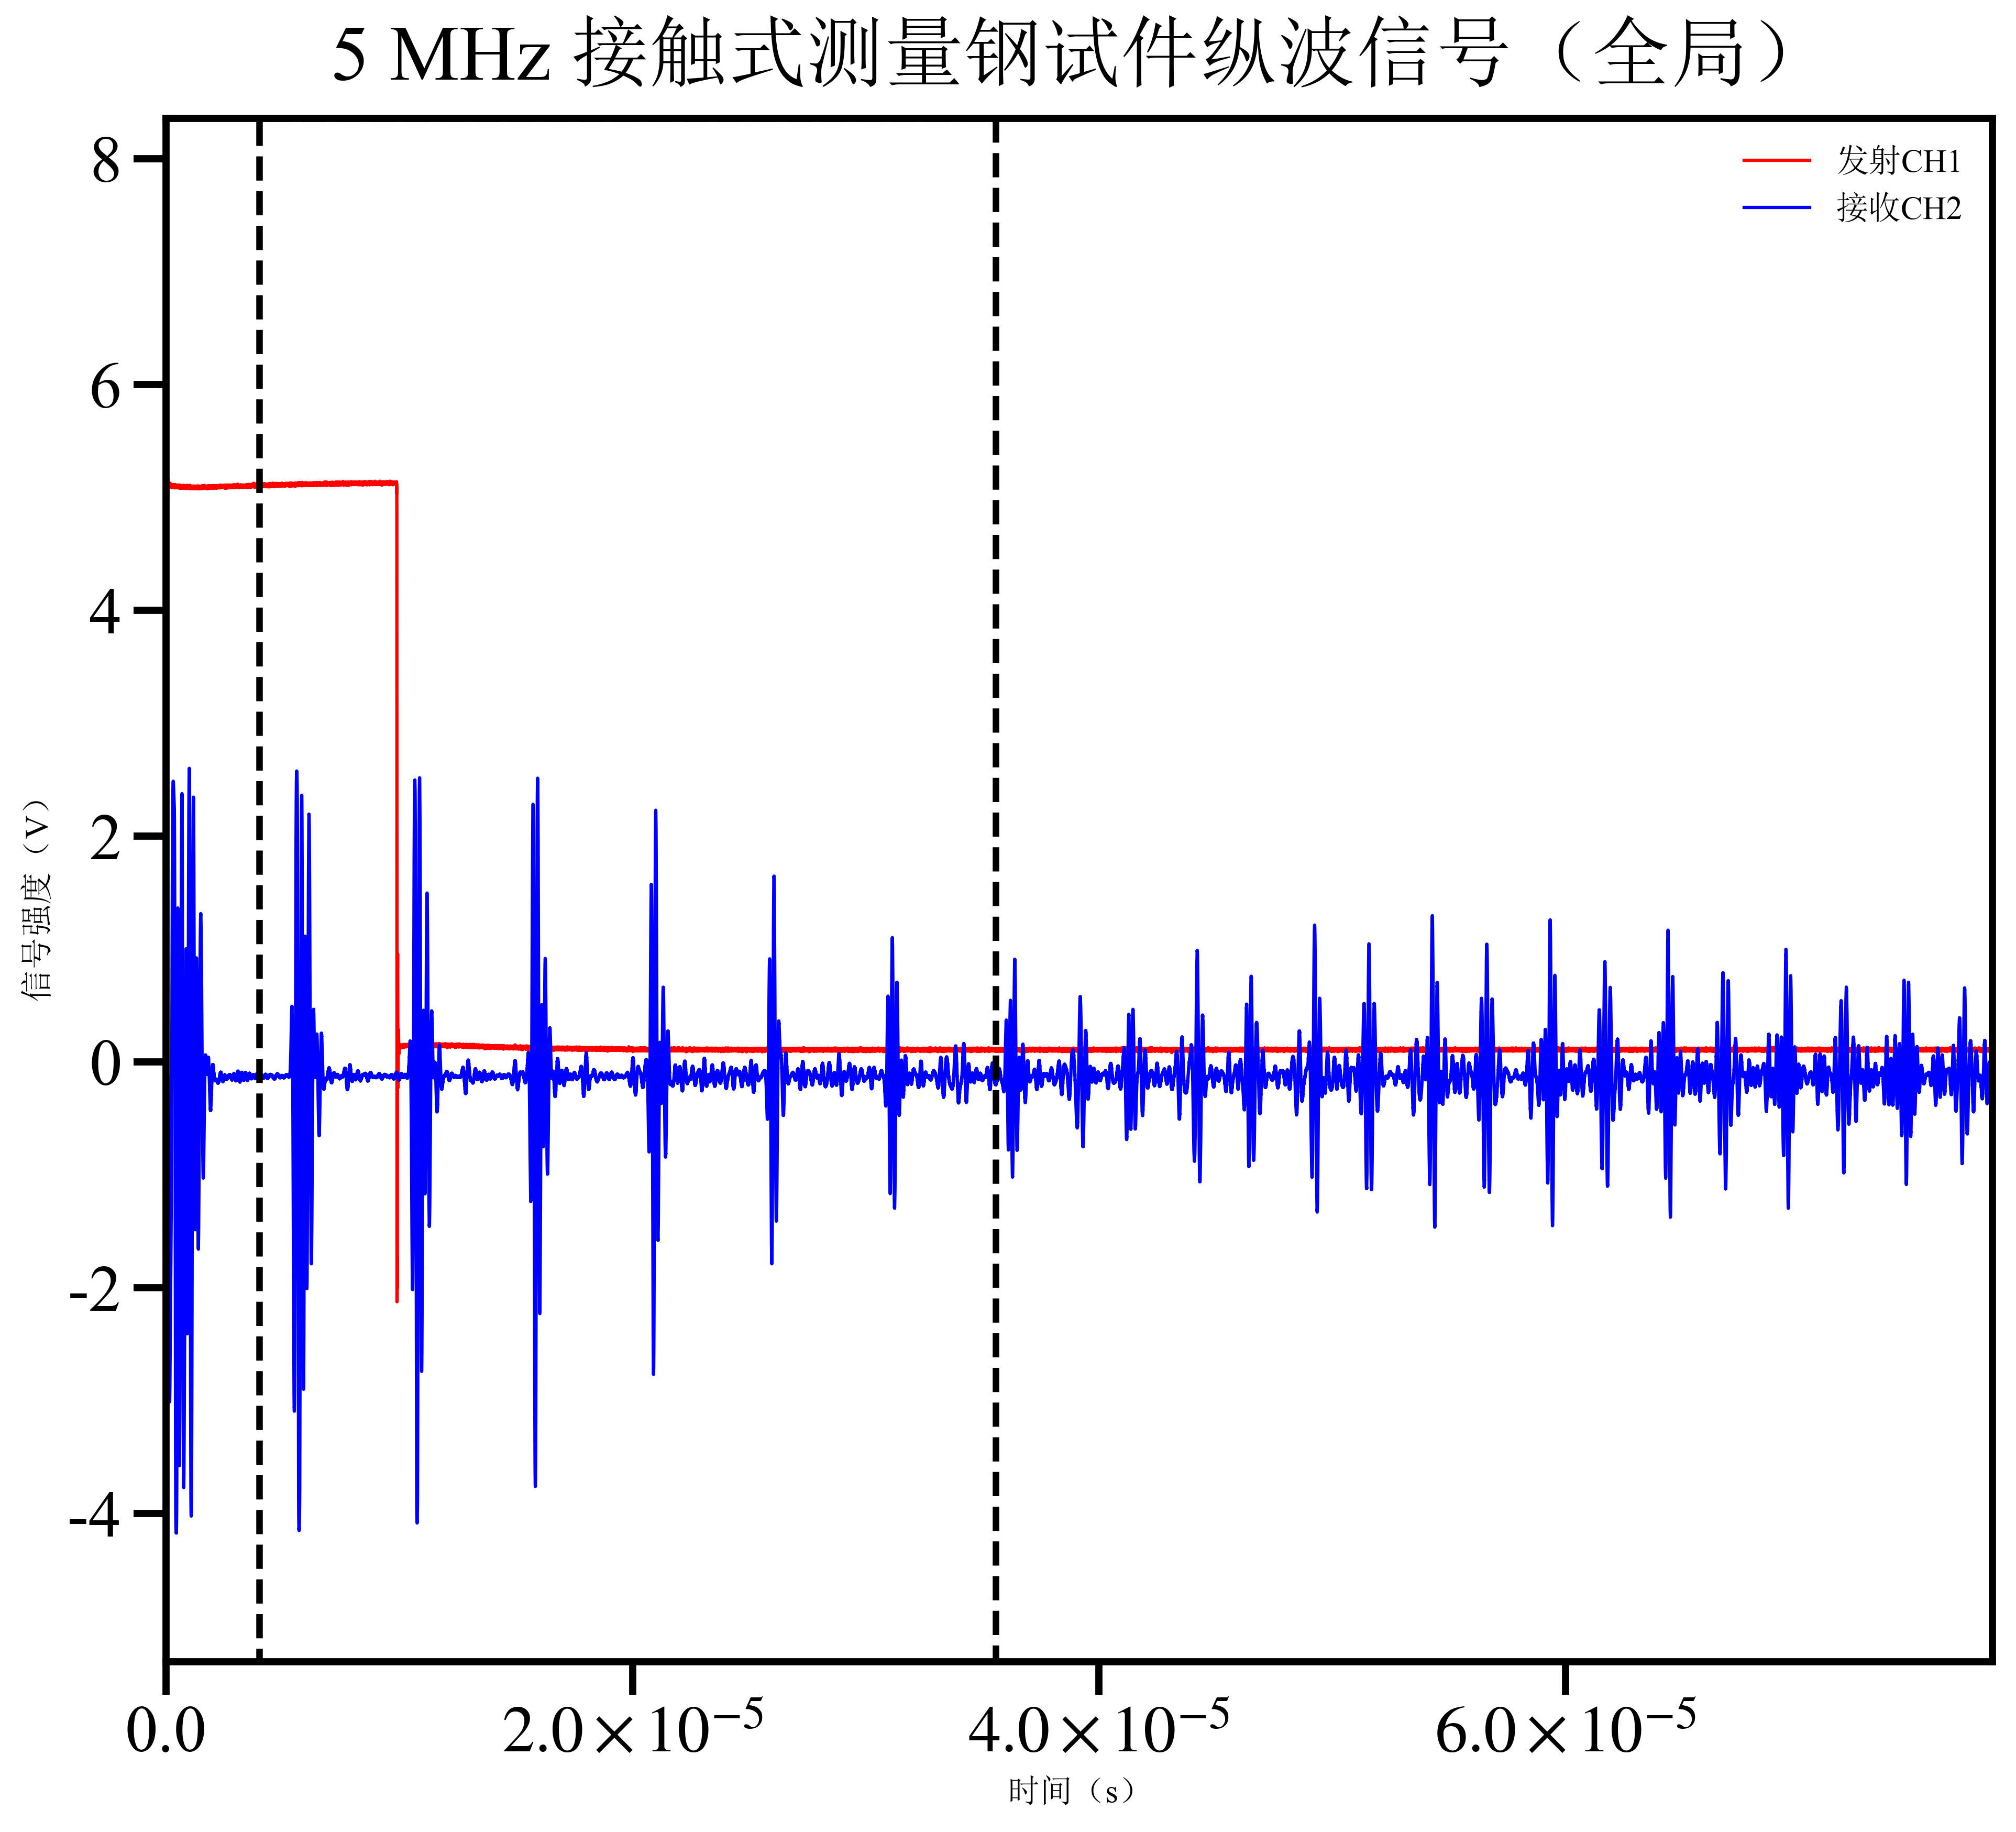
\includegraphics[width=\linewidth]{steel_5L_global.png}
  （a）输入输出信号全局图
\end{minipage}\hfill
\begin{minipage}[t]{0.48\textwidth}
  \centering
  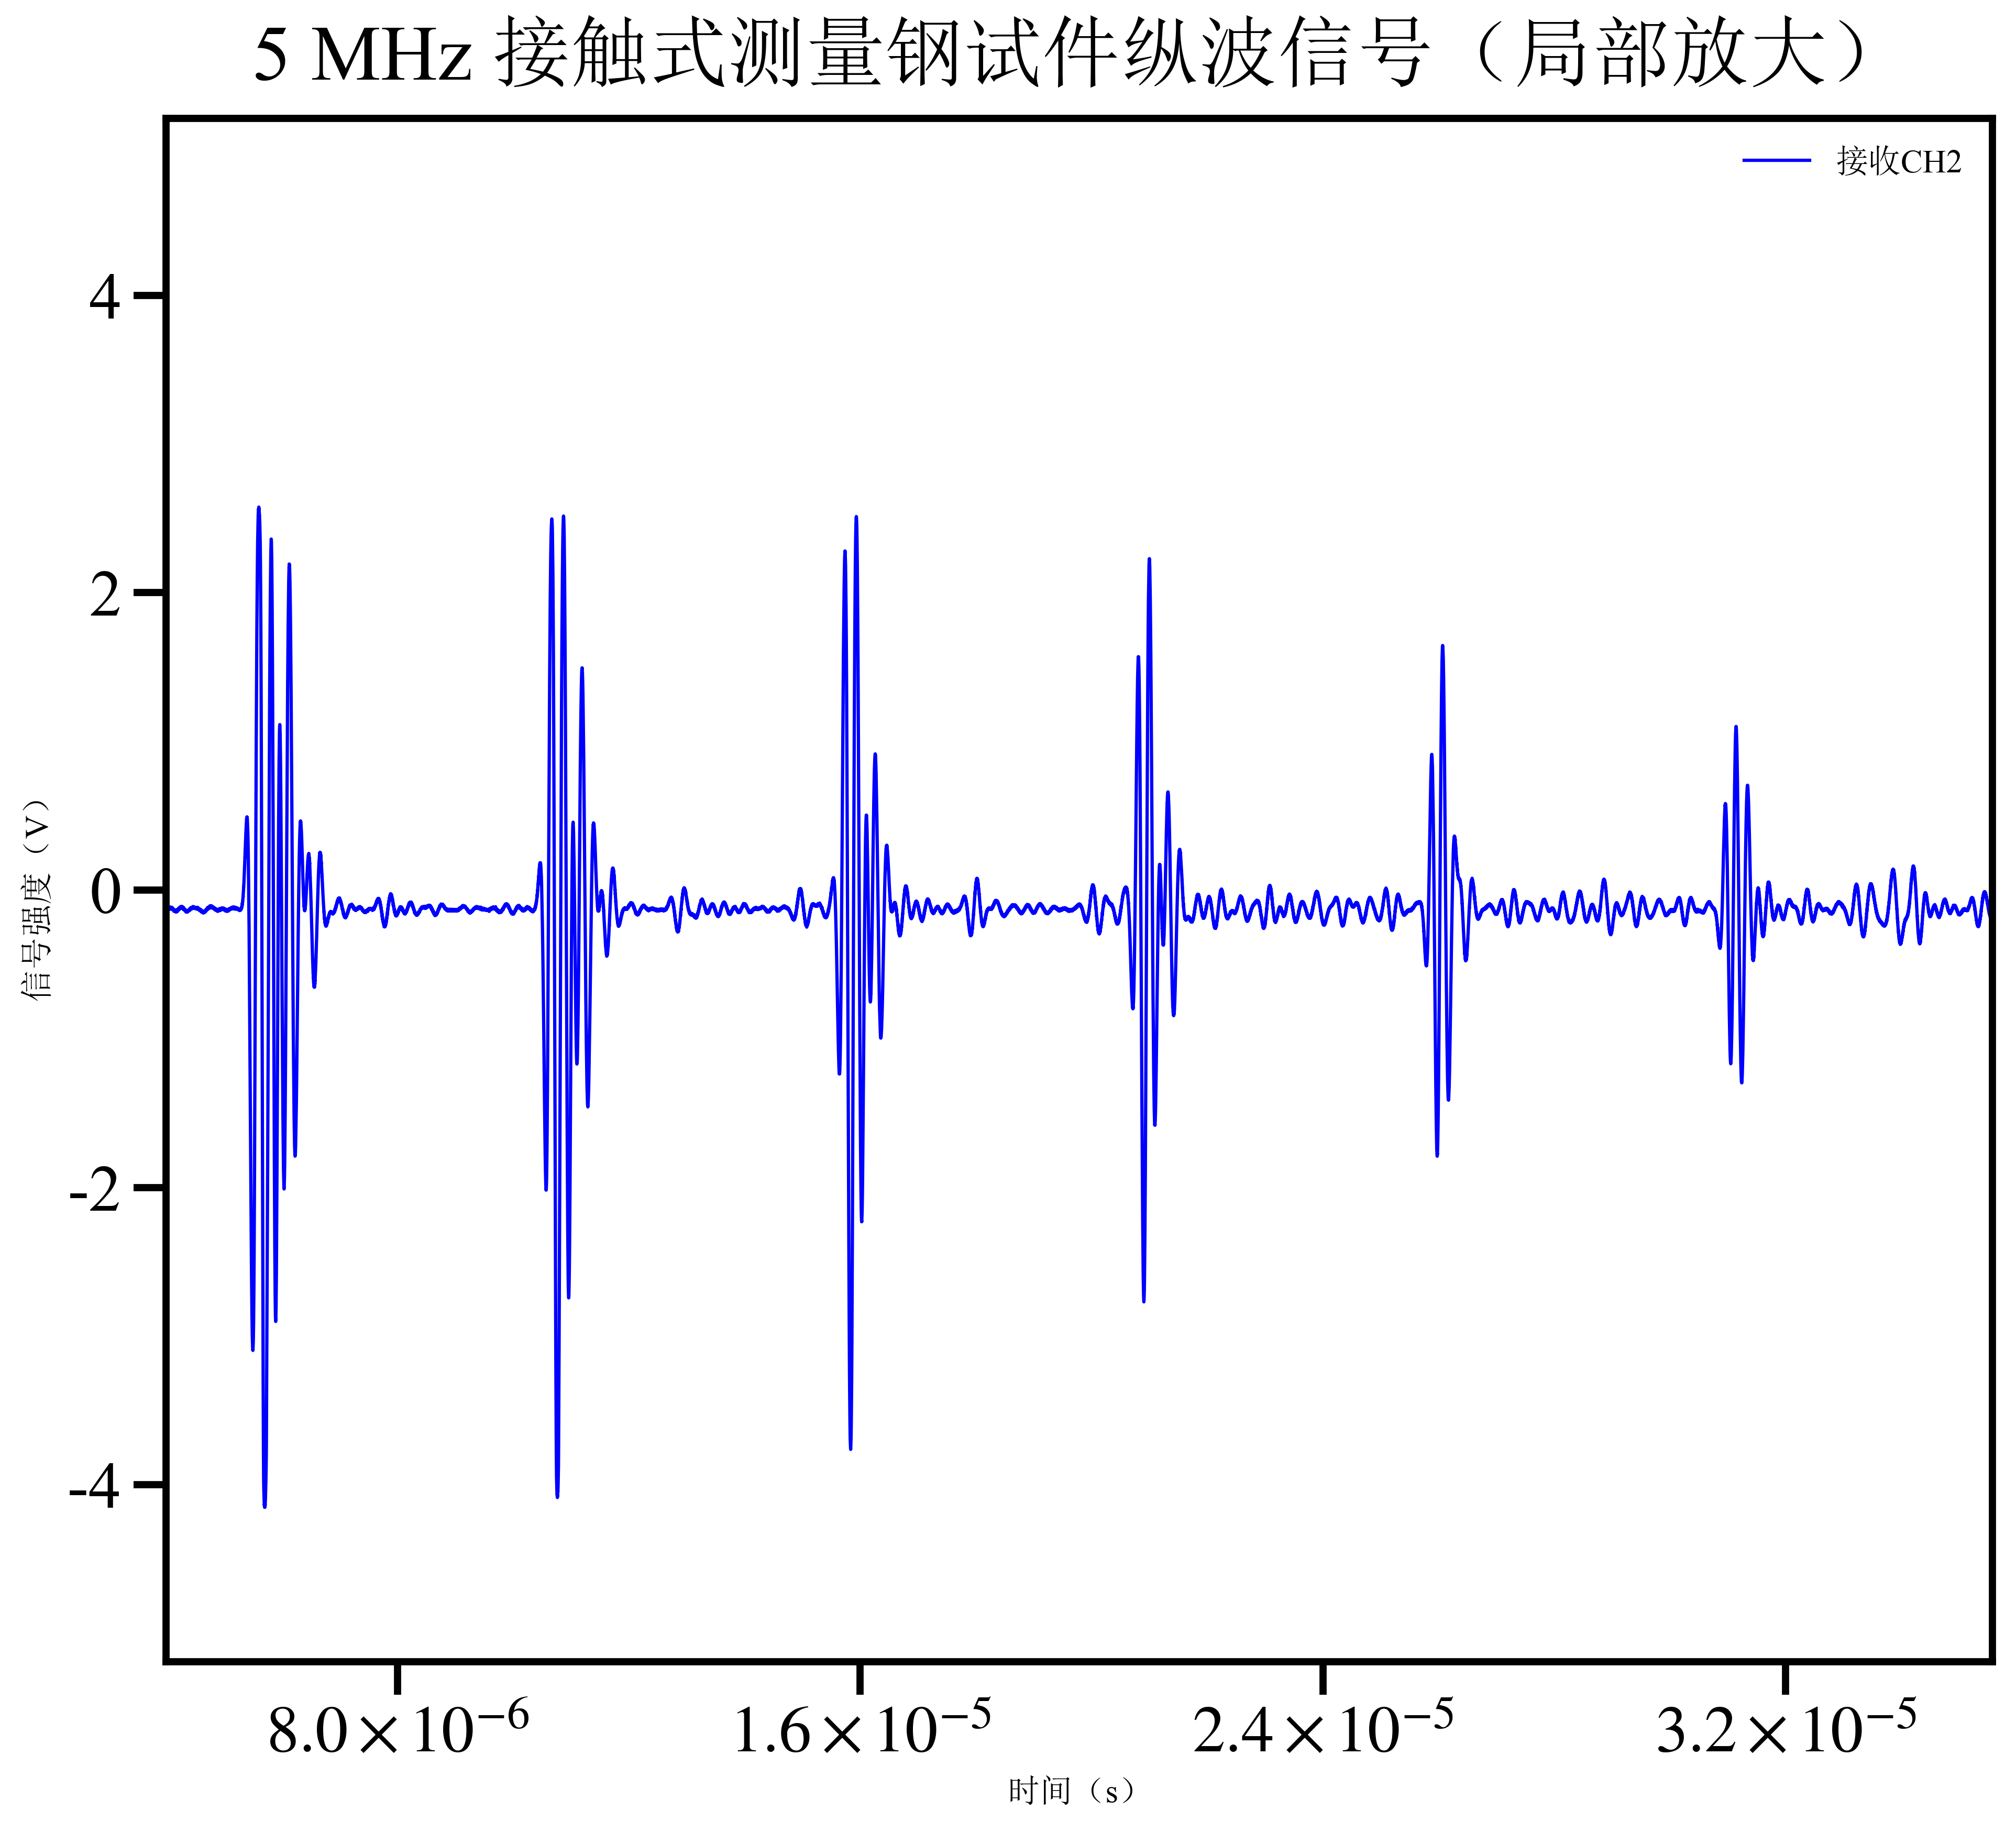
\includegraphics[width=\linewidth]{steel_5L_zoom.png}
  （b）输出信号局部放大图
\end{minipage}
\caption{5 MHz 接触式测量钢试件纵波波速时信号图}
\label{fig:exp2-steel-5}
\end{figure}

\begin{figure}[H]
\centering
\begin{minipage}[t]{0.48\textwidth}
  \centering
  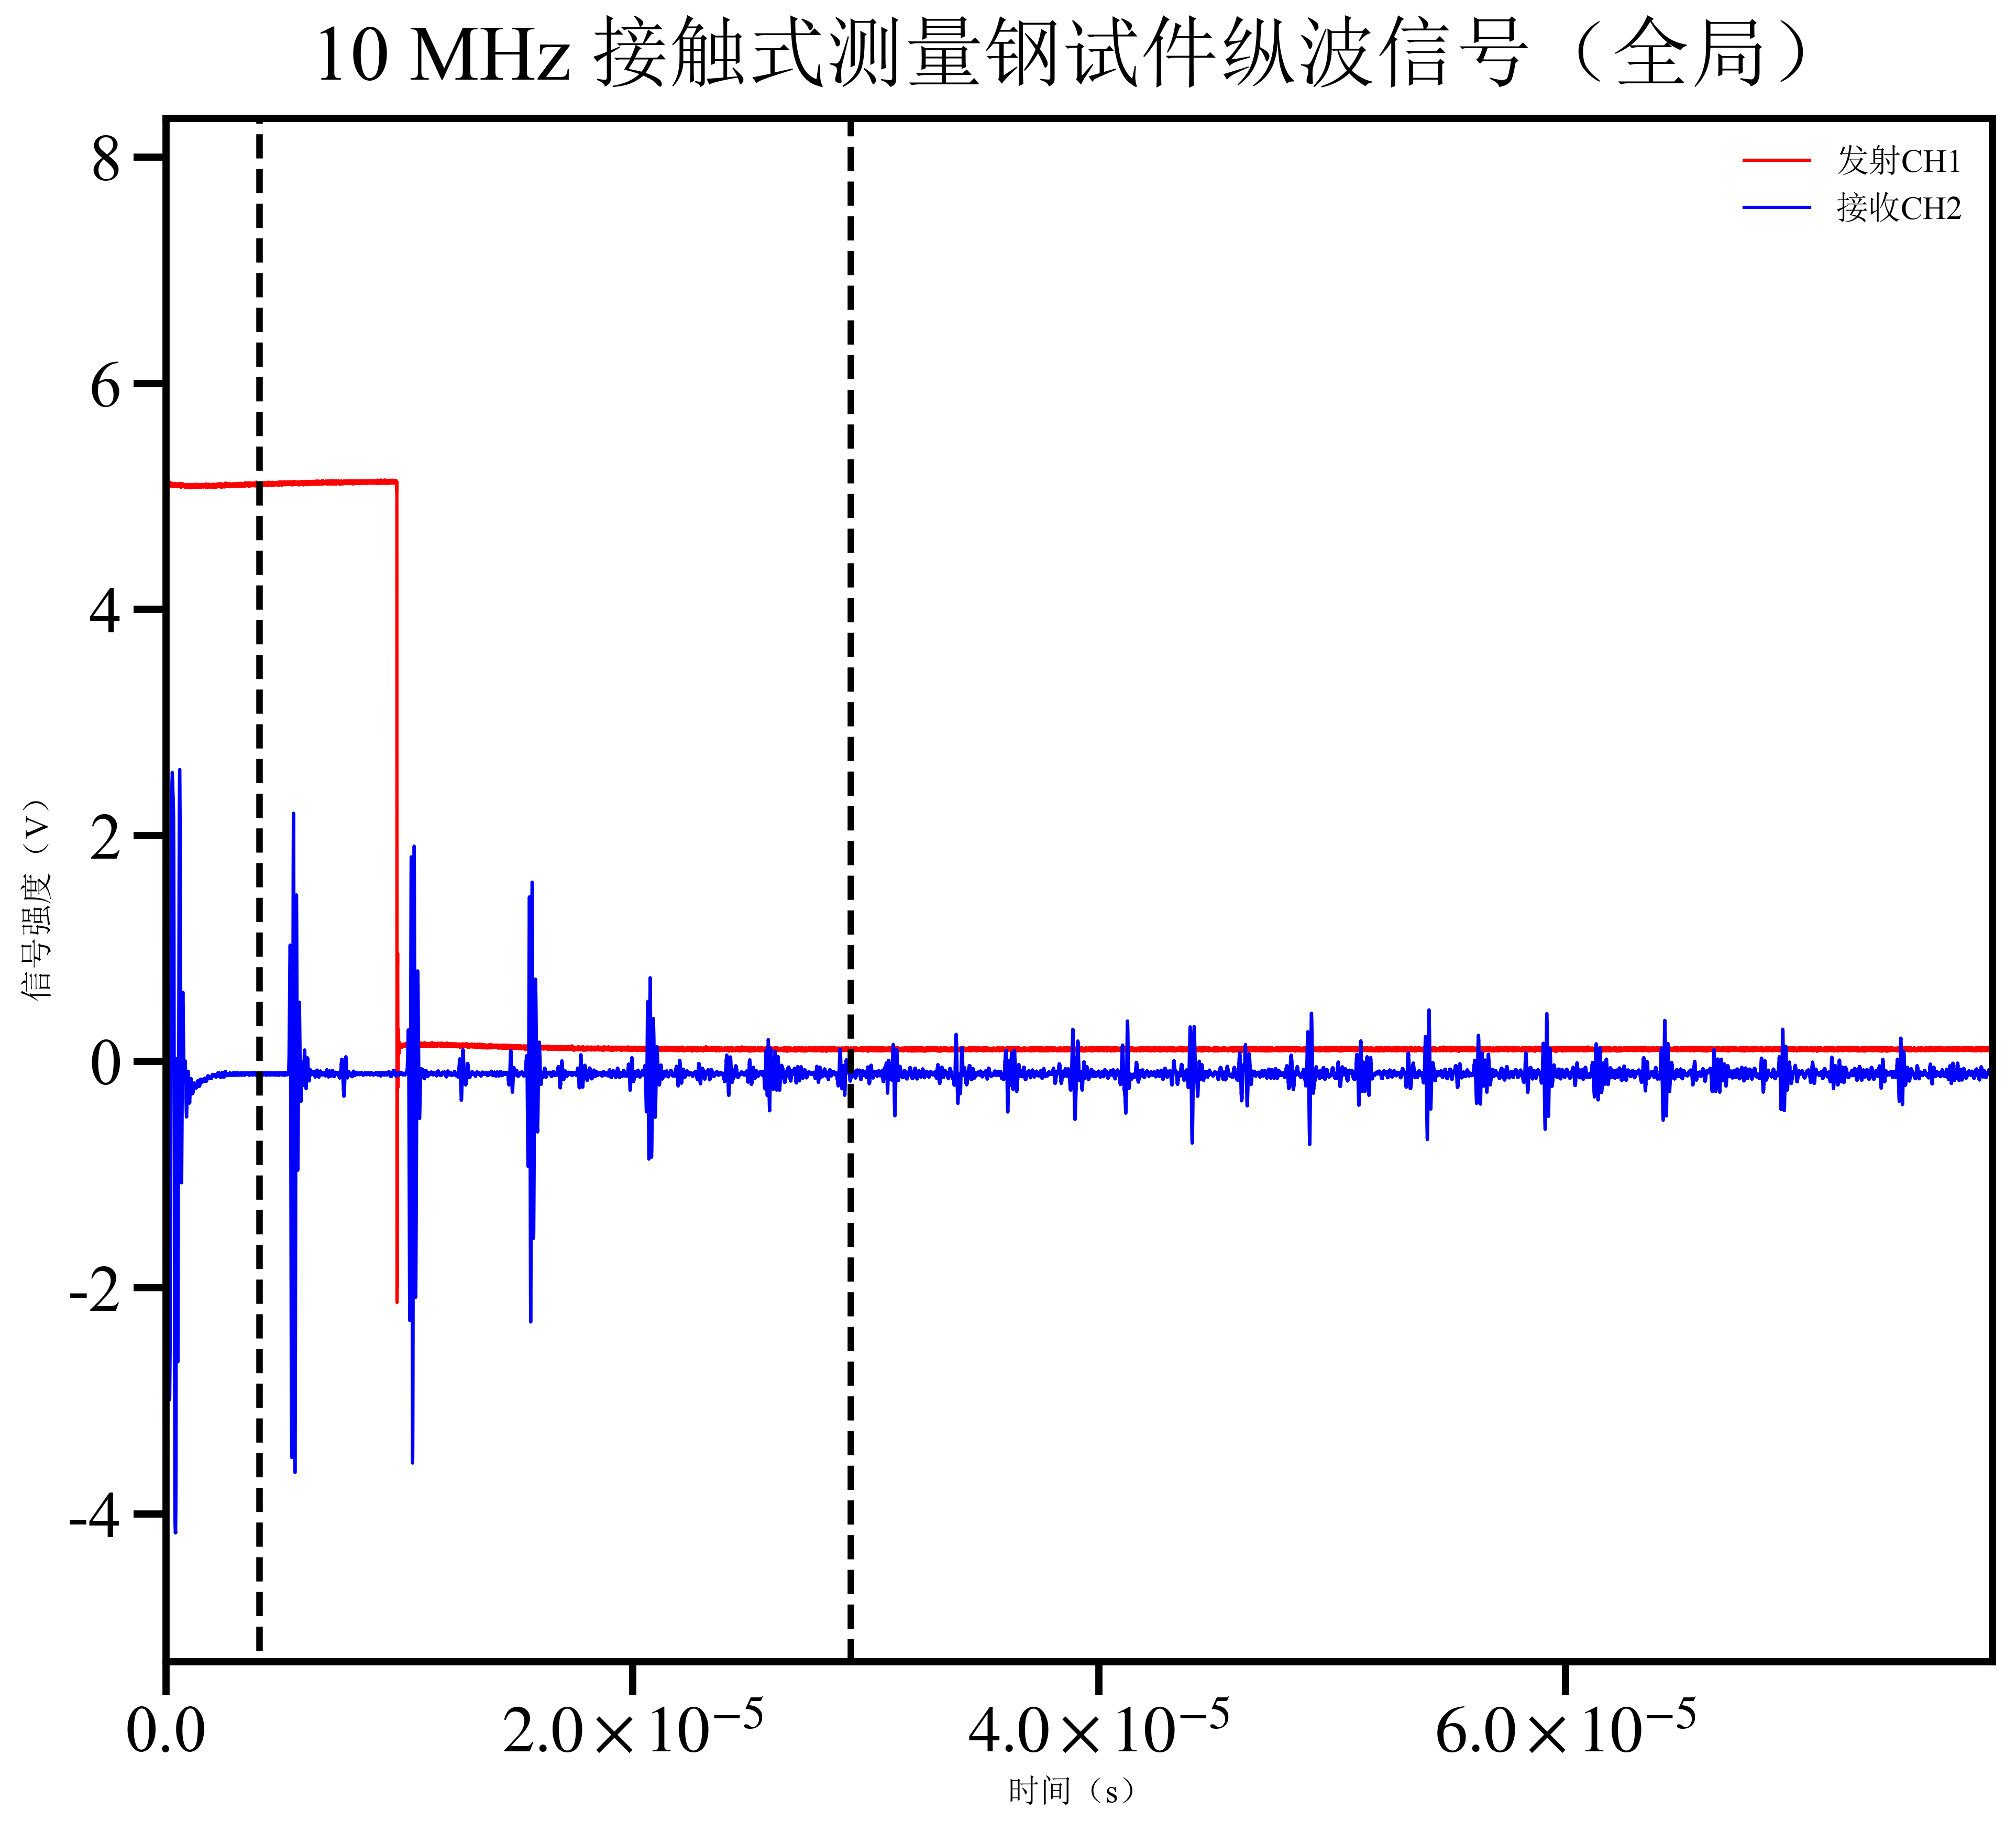
\includegraphics[width=\linewidth]{steel_10L_global.png}
  （a）输入输出信号全局图
\end{minipage}\hfill
\begin{minipage}[t]{0.48\textwidth}
  \centering
  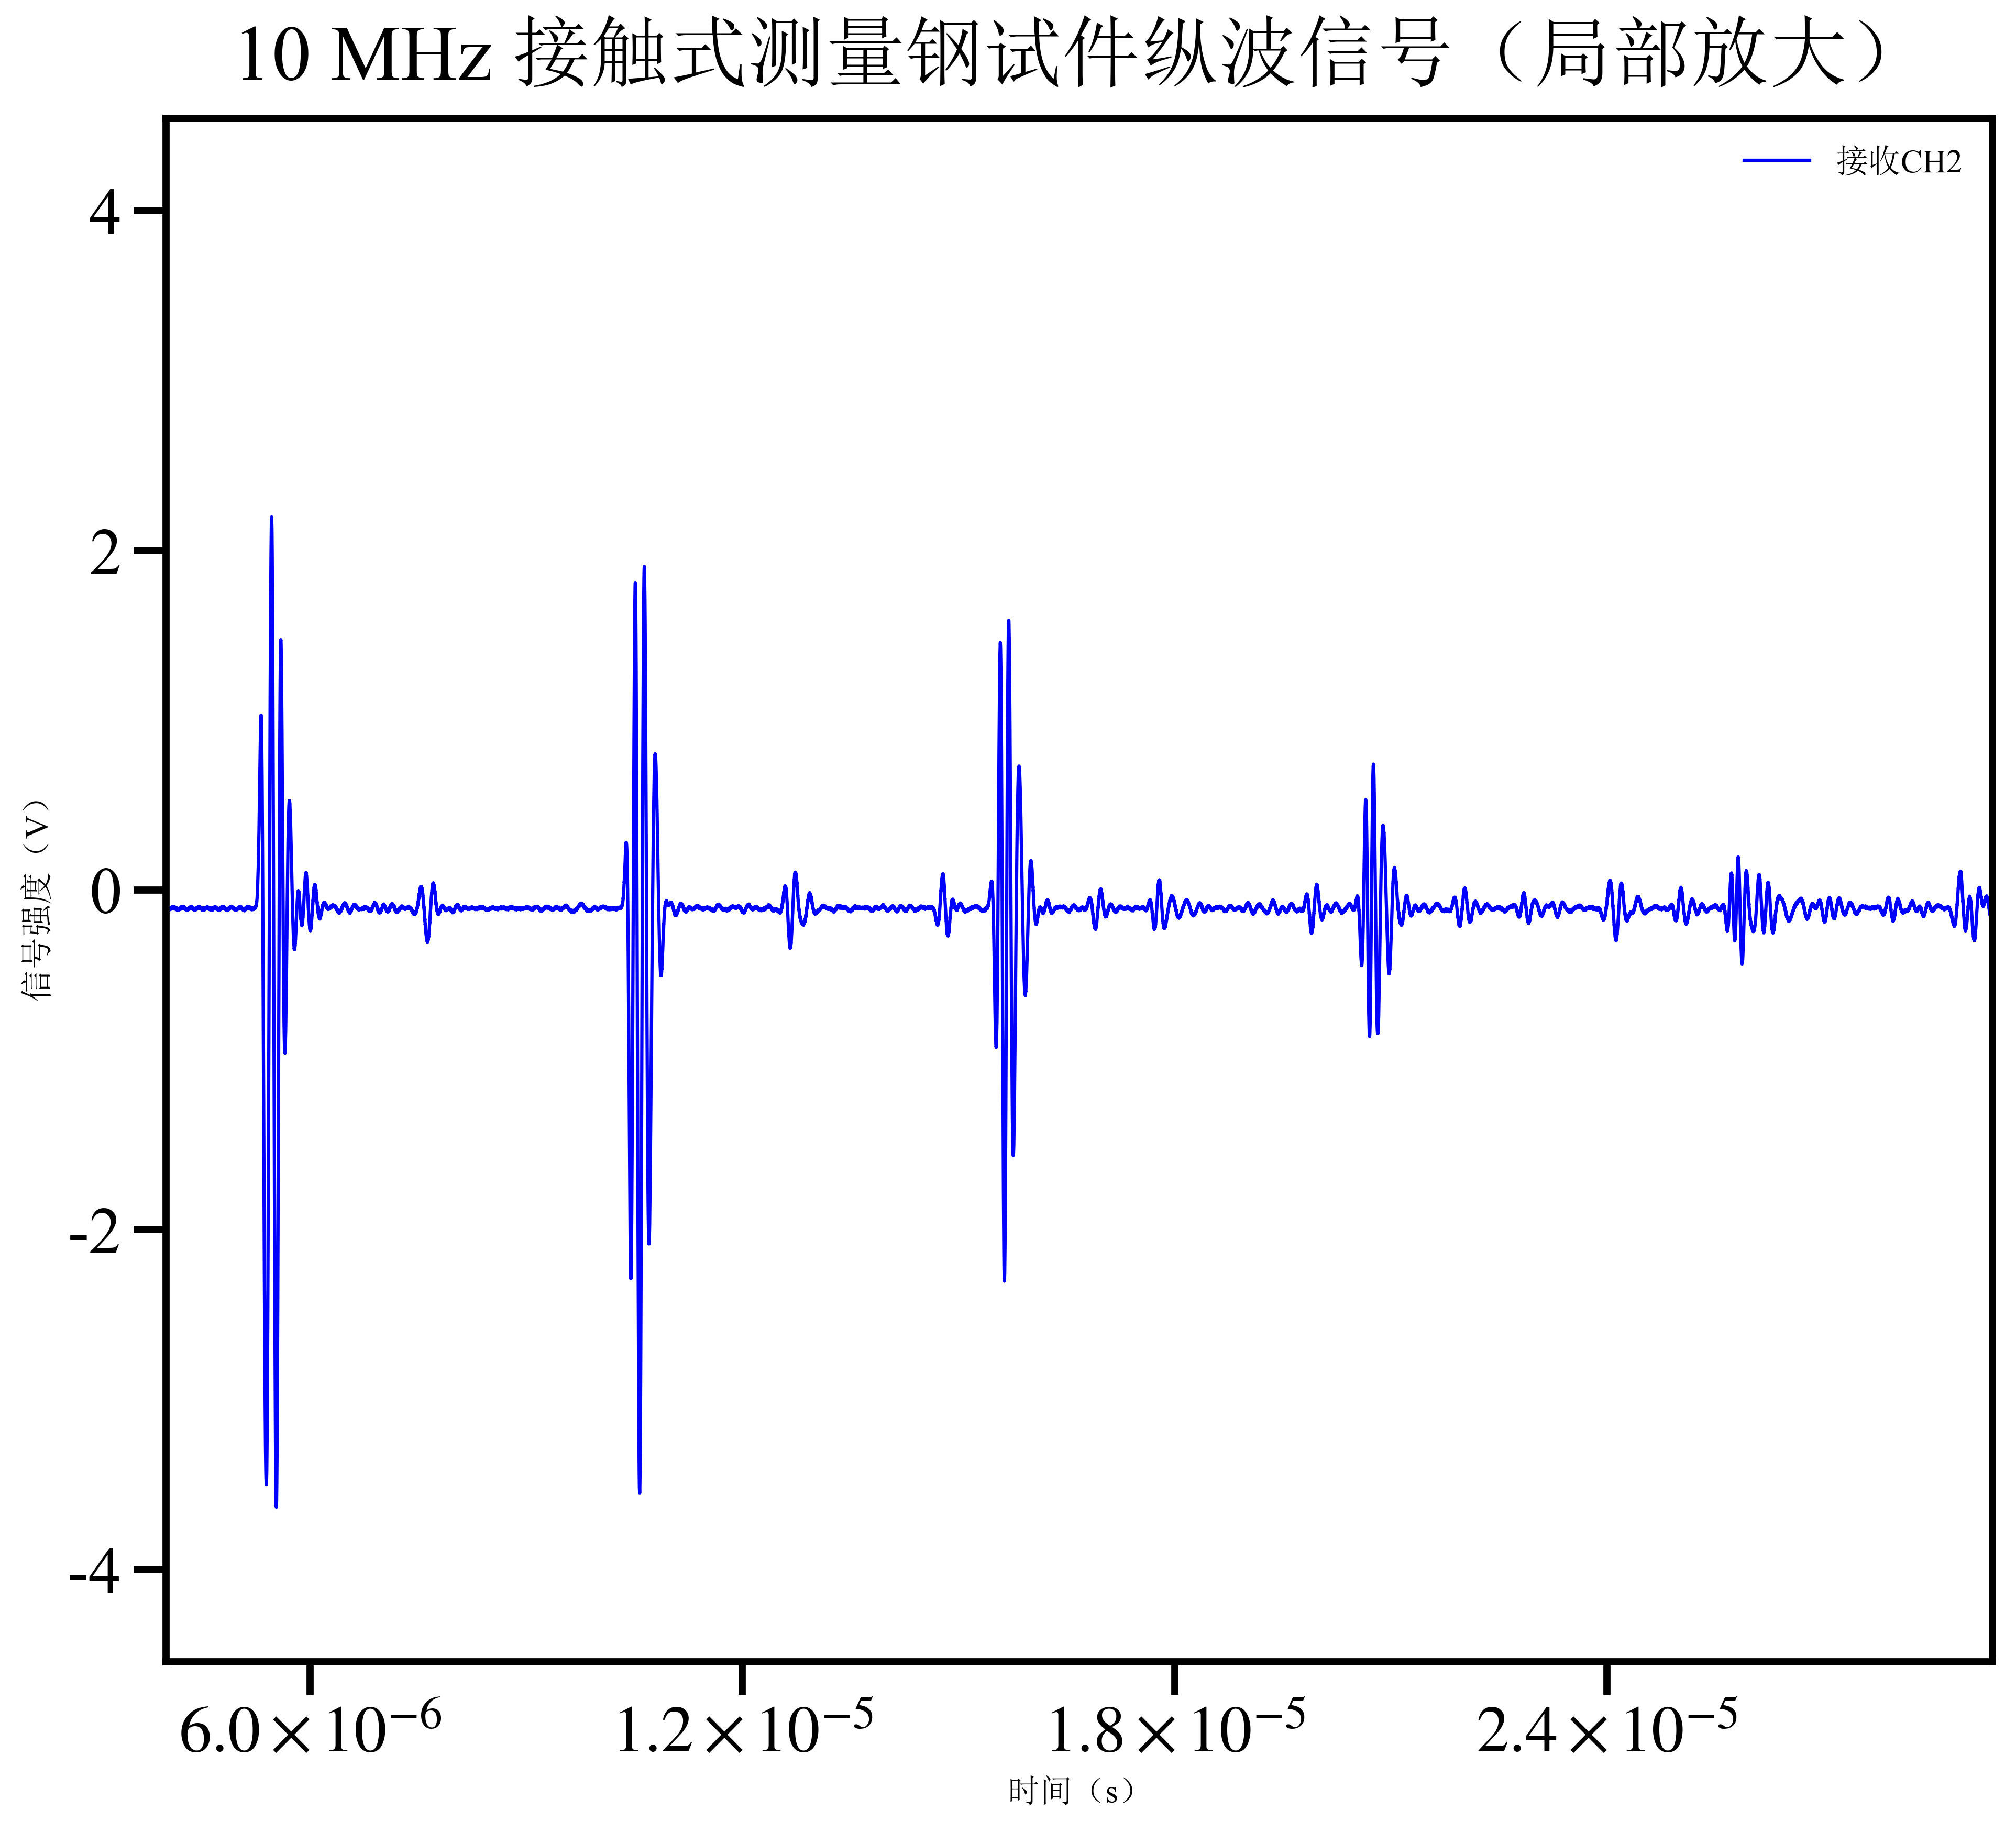
\includegraphics[width=\linewidth]{steel_10L_zoom.png}
  （b）输出信号局部放大图
\end{minipage}
\caption{10 MHz 接触式测量钢试件纵波波速时信号图}
\end{figure}

\begin{figure}[H]
\centering
\begin{minipage}[t]{0.48\textwidth}
  \centering
  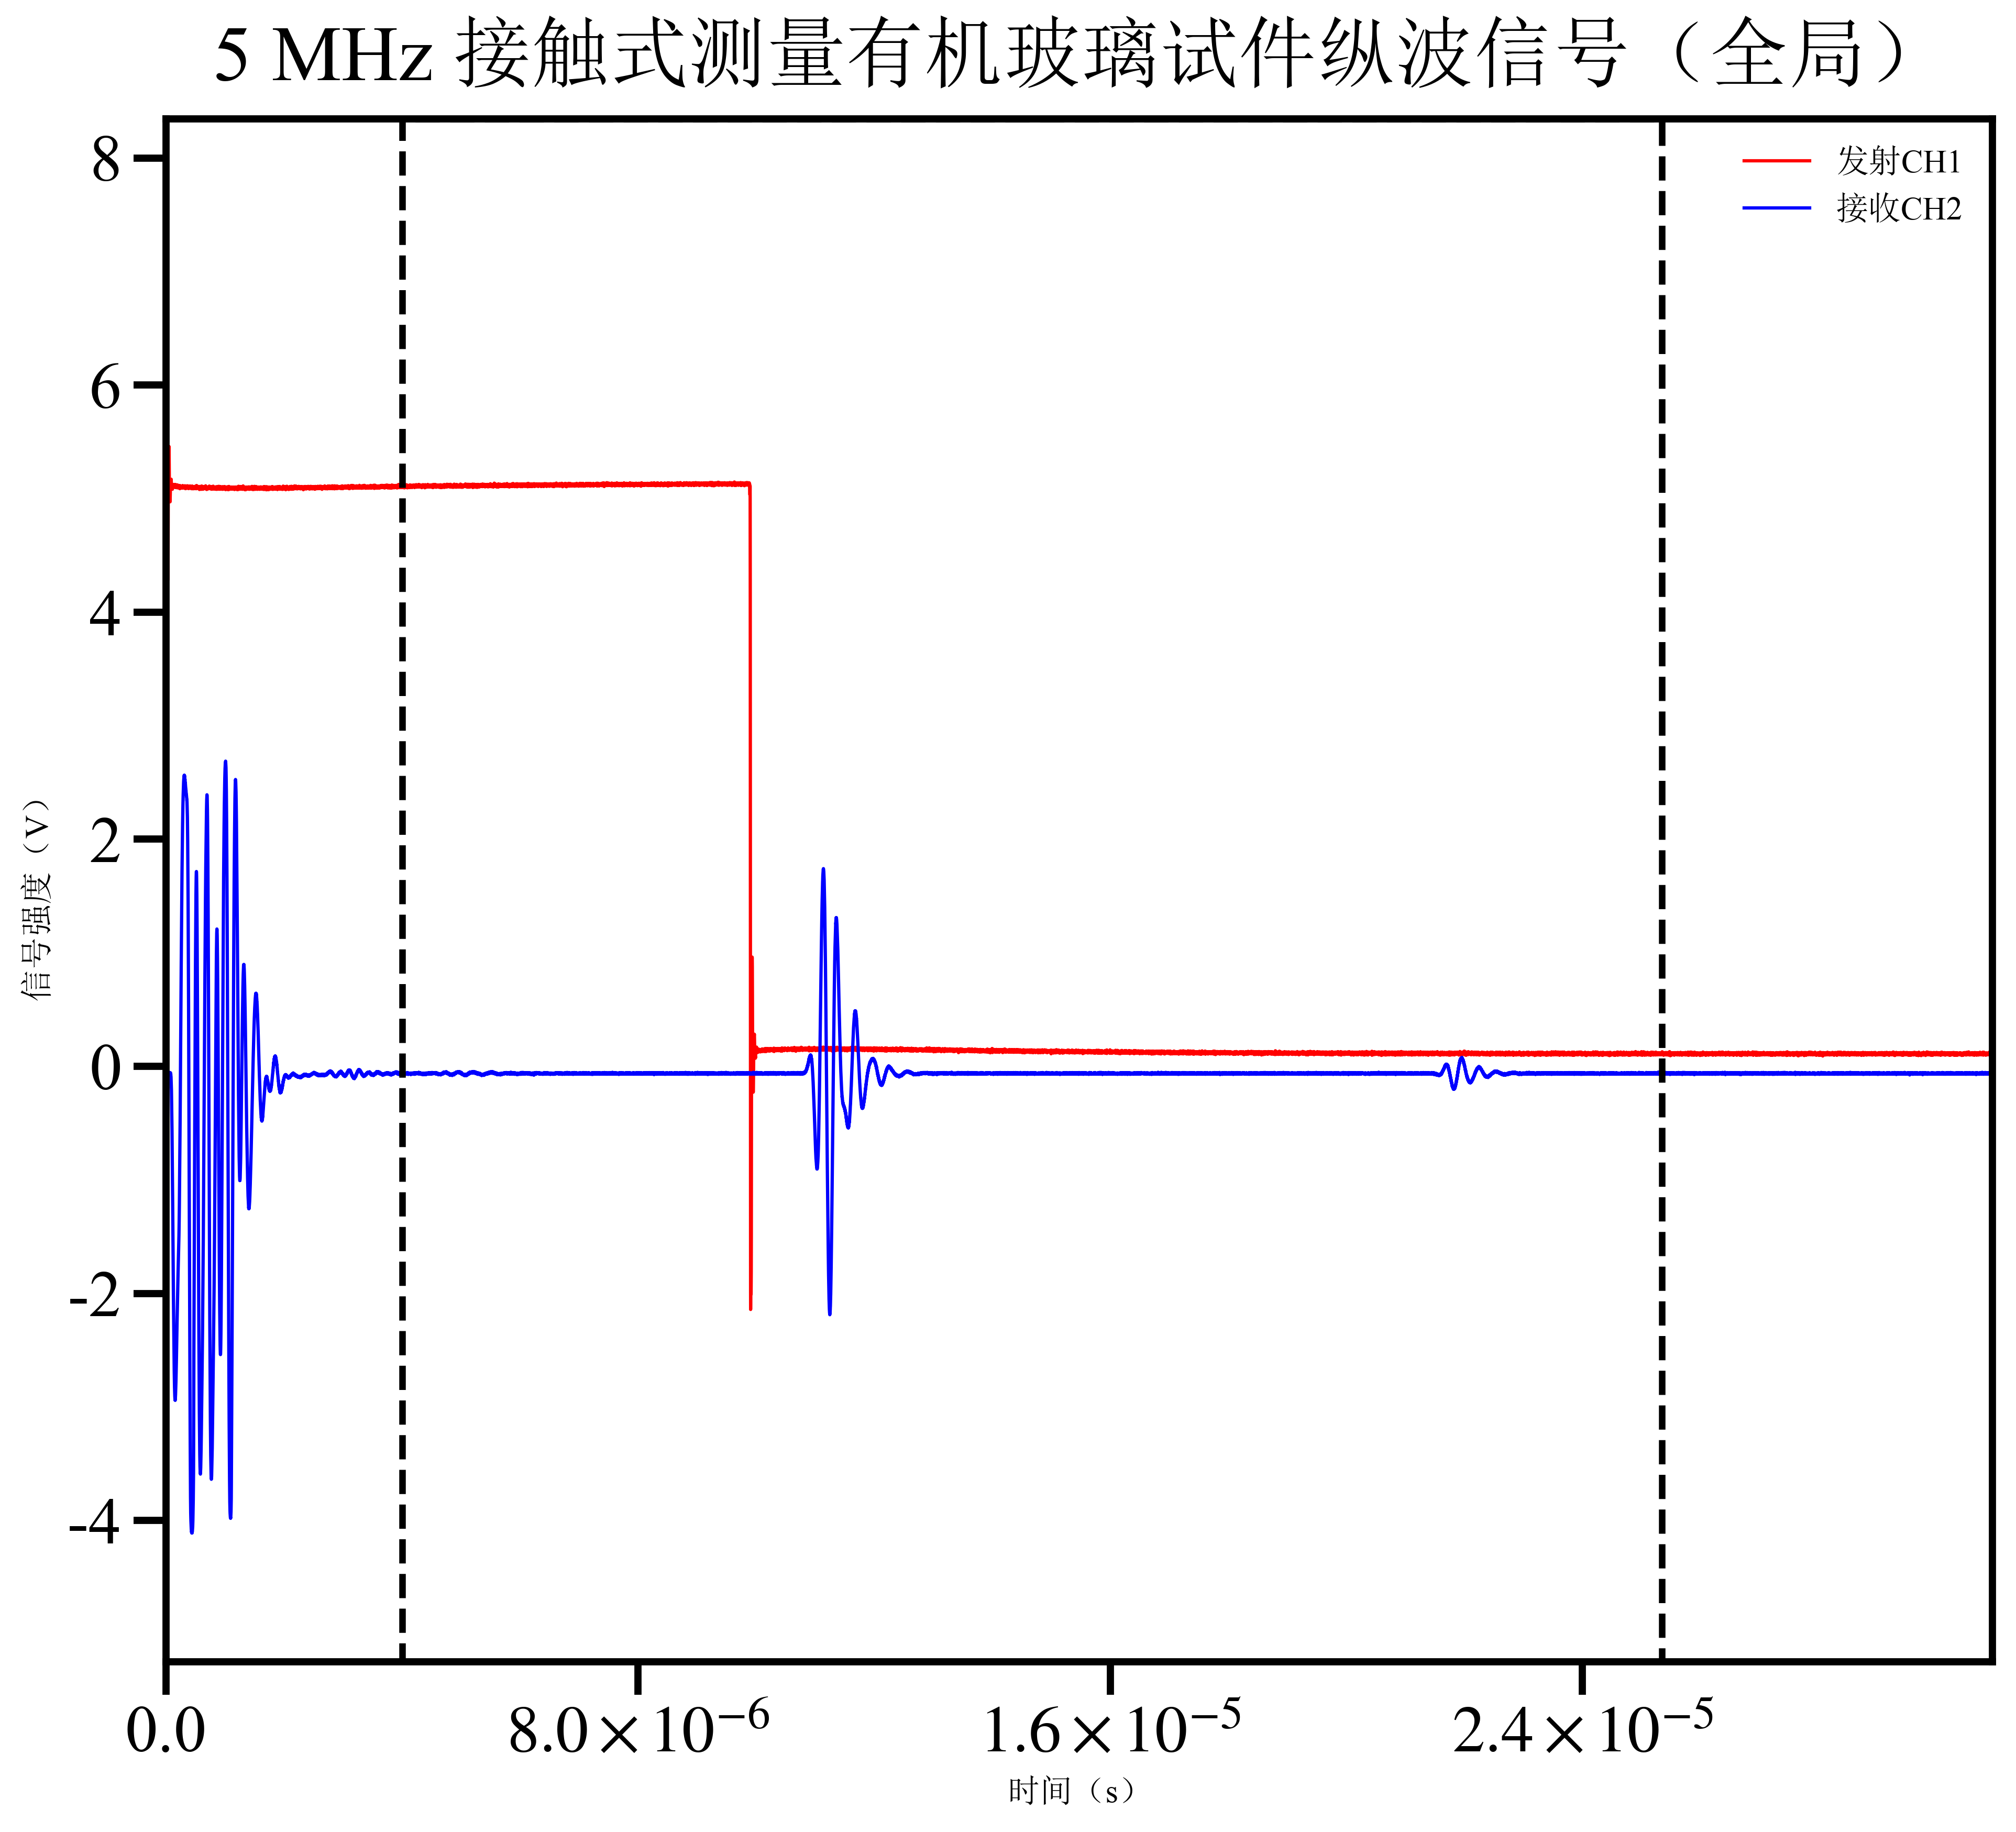
\includegraphics[width=\linewidth]{glass_5L_global.png}
  （a）输入输出信号全局图
\end{minipage}\hfill
\begin{minipage}[t]{0.48\textwidth}
  \centering
  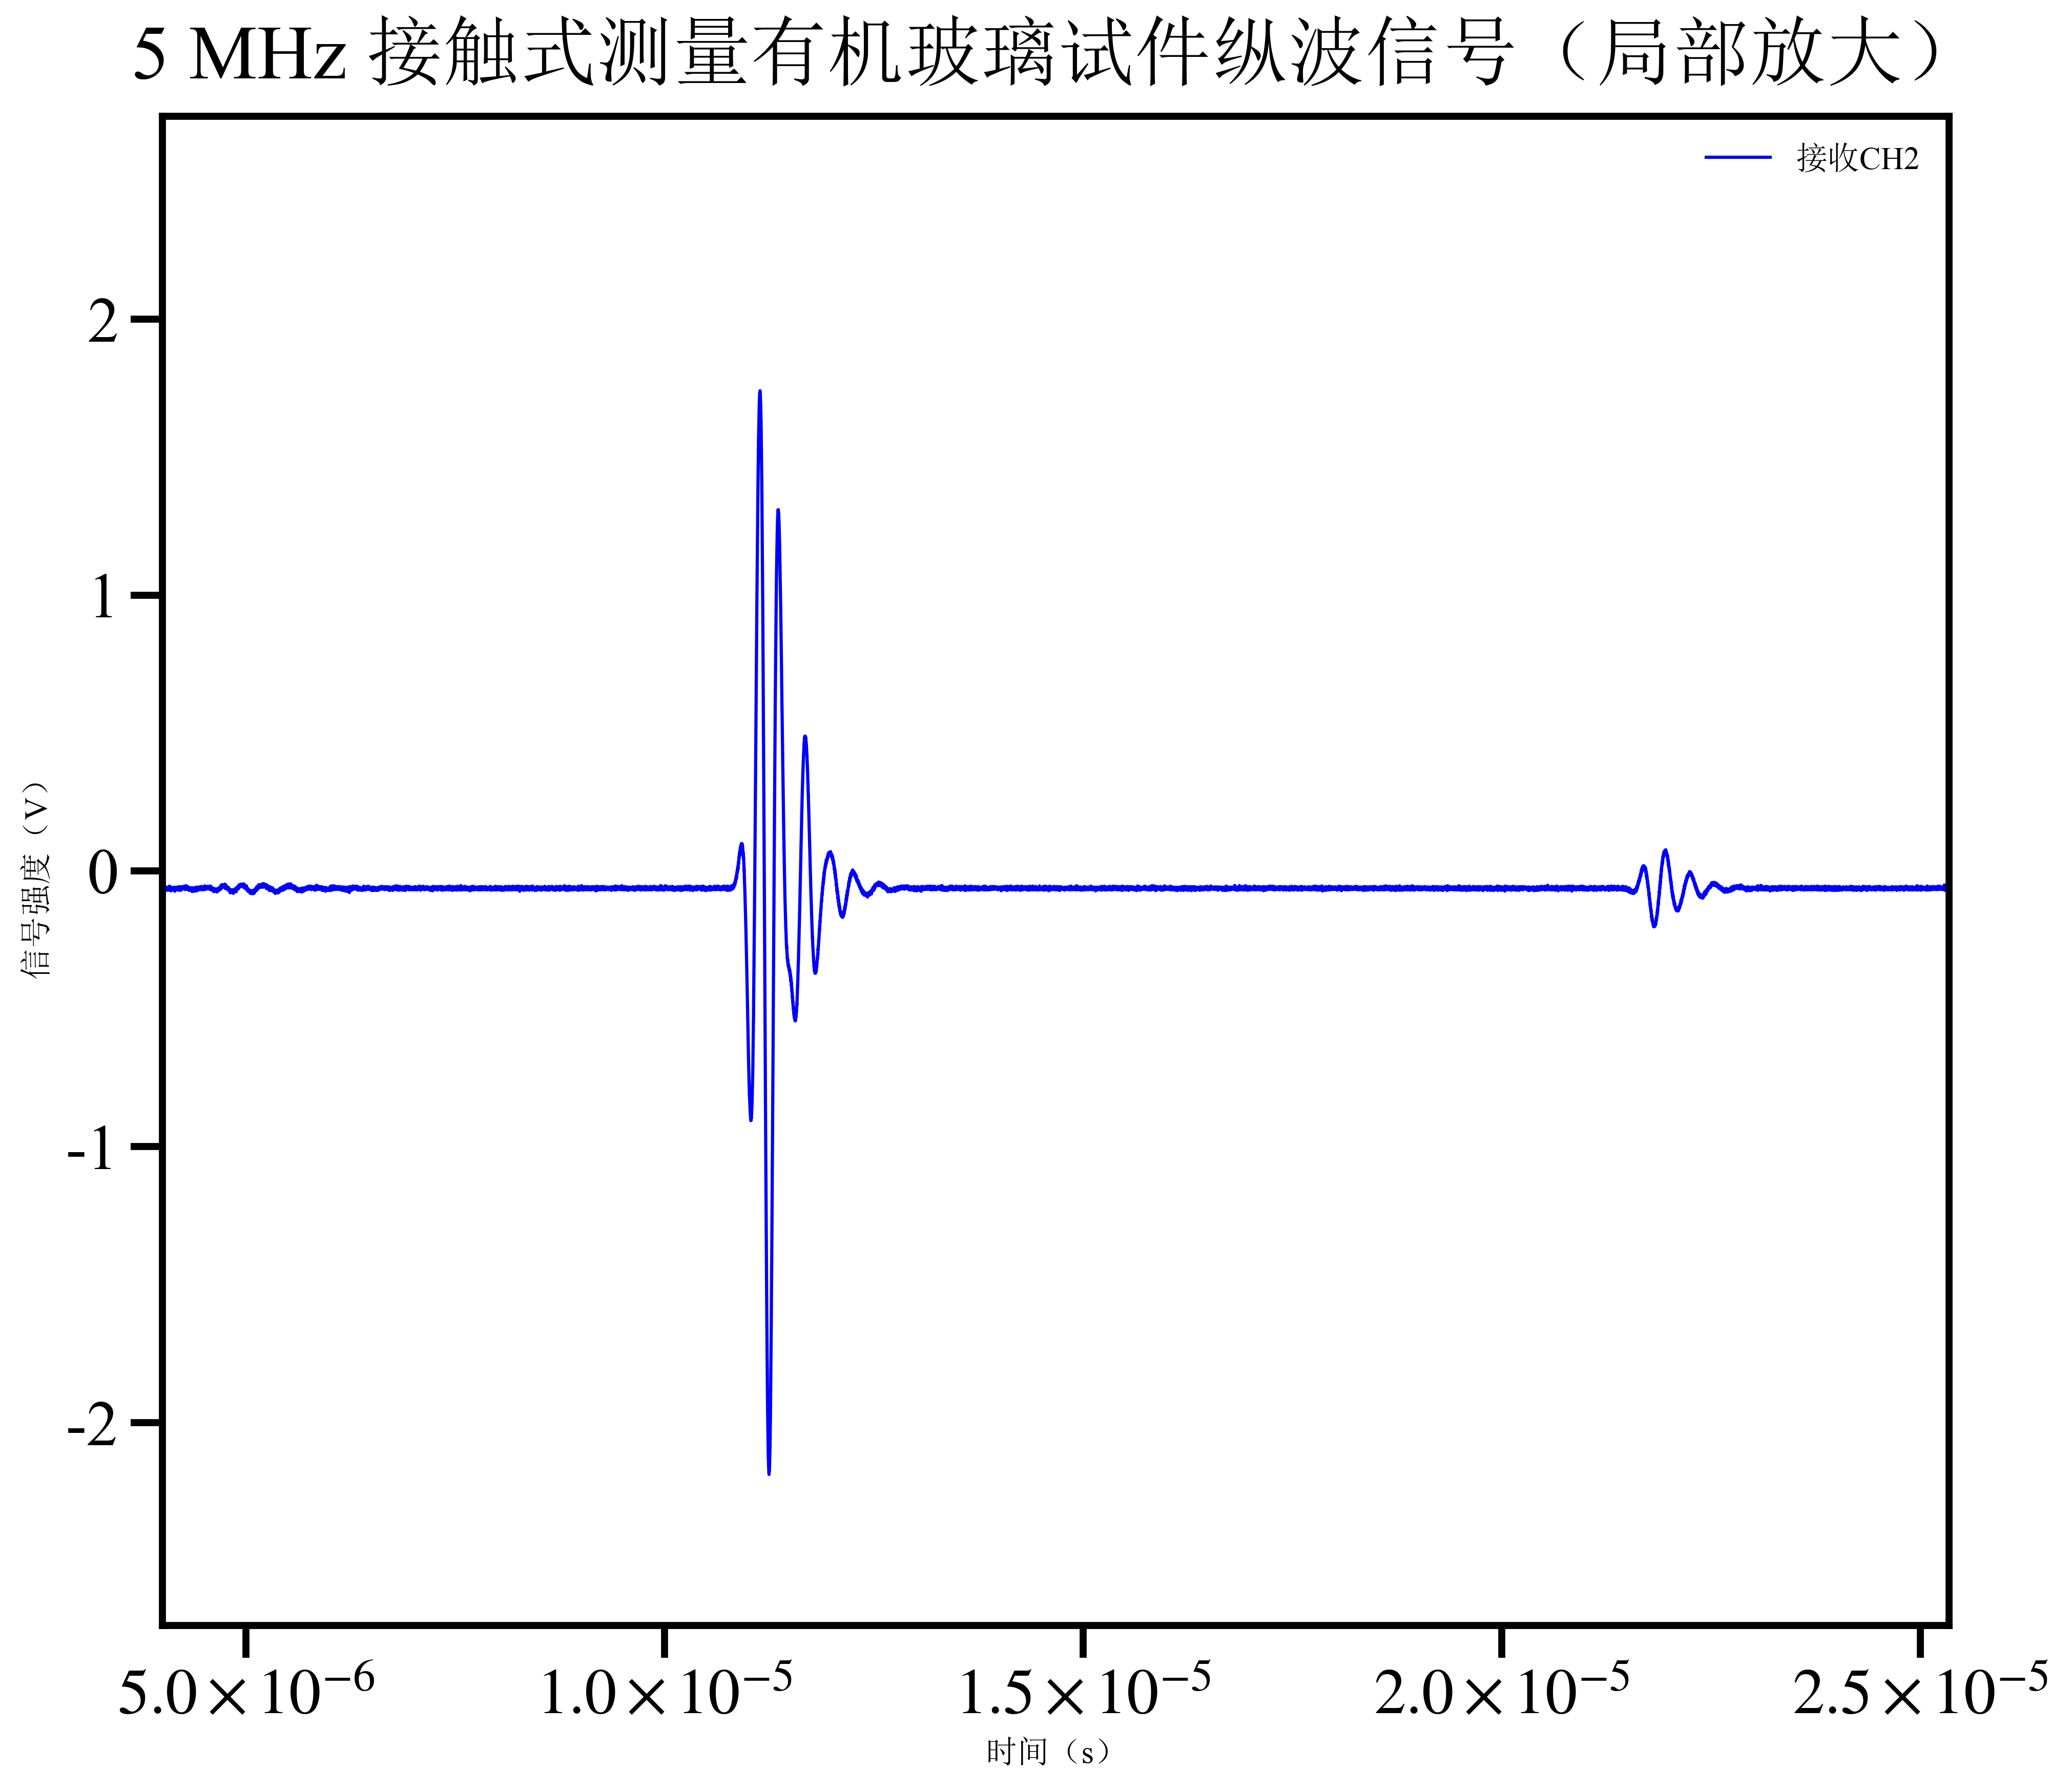
\includegraphics[width=\linewidth]{glass_5L_zoom.png}
  （b）输出信号局部放大图
\end{minipage}
\caption{5 MHz 接触式测量有机玻璃试件纵波波速时信号图}
\label{fig:exp2-og-5}
\end{figure}

\begin{table}[H]
\centering
\caption{5 MHz 与 10 MHz 接触式测量的纵波回波时间差}
\label{tab:exp2-frequency-time}
\begin{tabular}{lcc}
\toprule
材料 & 探头频率 & $\Delta t_L$（$\mu$s）\\
\midrule
钢 & 5 MHz & 5.06\\
钢 & 10 MHz & 5.06\\
有机玻璃 & 5 MHz & 10.57\\
有机玻璃 & 10 MHz & 10.90\\
\bottomrule
\end{tabular}
\end{table}

有机玻璃 10 MHz 信号中仅检出一个清晰回波，其 $\Delta t_L$ 取入射波到该回波的时间差。根据表\ref{tab:exp2-density}中的厚度及表\ref{tab:exp2-frequency-time}中的时间差，分别计算四种工况下的纵波波速：
\begin{subequations}
\begin{align}
  C_{L,st}^{5\mathrm{MHz}}&=\frac{2h_{st}}{\Delta t_{L,st}^{5\mathrm{MHz}}}\times10^3
  =5949\ \mathrm{m/s},\\
  C_{L,st}^{10\mathrm{MHz}}&=\frac{2h_{st}}{\Delta t_{L,st}^{10\mathrm{MHz}}}\times10^3
  =5949\ \mathrm{m/s},\\
  C_{L,og}^{5\mathrm{MHz}}&=\frac{2h_{og}}{\Delta t_{L,og}^{5\mathrm{MHz}}}\times10^3
  =2668\ \mathrm{m/s},\\
  C_{L,og}^{10\mathrm{MHz}}&=\frac{2h_{og}}{\Delta t_{L,og}^{10\mathrm{MHz}}}\times10^3
  =2587\ \mathrm{m/s}.
\end{align}
\end{subequations}
将本结果与水浸法结果比较，分析测量方法及探头频率对波速、杂波和读数的影响。
钢试件 5 MHz 与 10 MHz 接触式测量所得纵波波速均为 $5949\,\mathrm{m/s}$，与水浸法结果 $5960\,\mathrm{m/s}$ 仅差 $0.2\%$，测量方法与探头频率对钢试件结果的影响很小。有机玻璃 5 MHz 接触式结果为 $2668\,\mathrm{m/s}$；10 MHz 信号衰减明显，仅检出单个回波，估算值为 $2587\,\mathrm{m/s}$，仅供参考。高频探头脉冲窄、分辨力高，但材料衰减随频率升高急剧增大，在有机玻璃中尤为明显。

\subsection{接触式测量有机玻璃纵波的衰减系数}
利用试件上下表面反射波振幅的关系，可以得到纵波在有机玻璃中的衰减系数。基于图\ref{fig:exp2-og-5}和图\ref{fig:exp2-og-10}读取不同时间下的波峰数值，将数据代入公式\eqref{eq:exp2-attenuation}，结果填入表\ref{tab:exp2-frequency-attenuation}。

\begin{figure}[H]
\centering
\begin{minipage}[t]{0.48\textwidth}
  \centering
  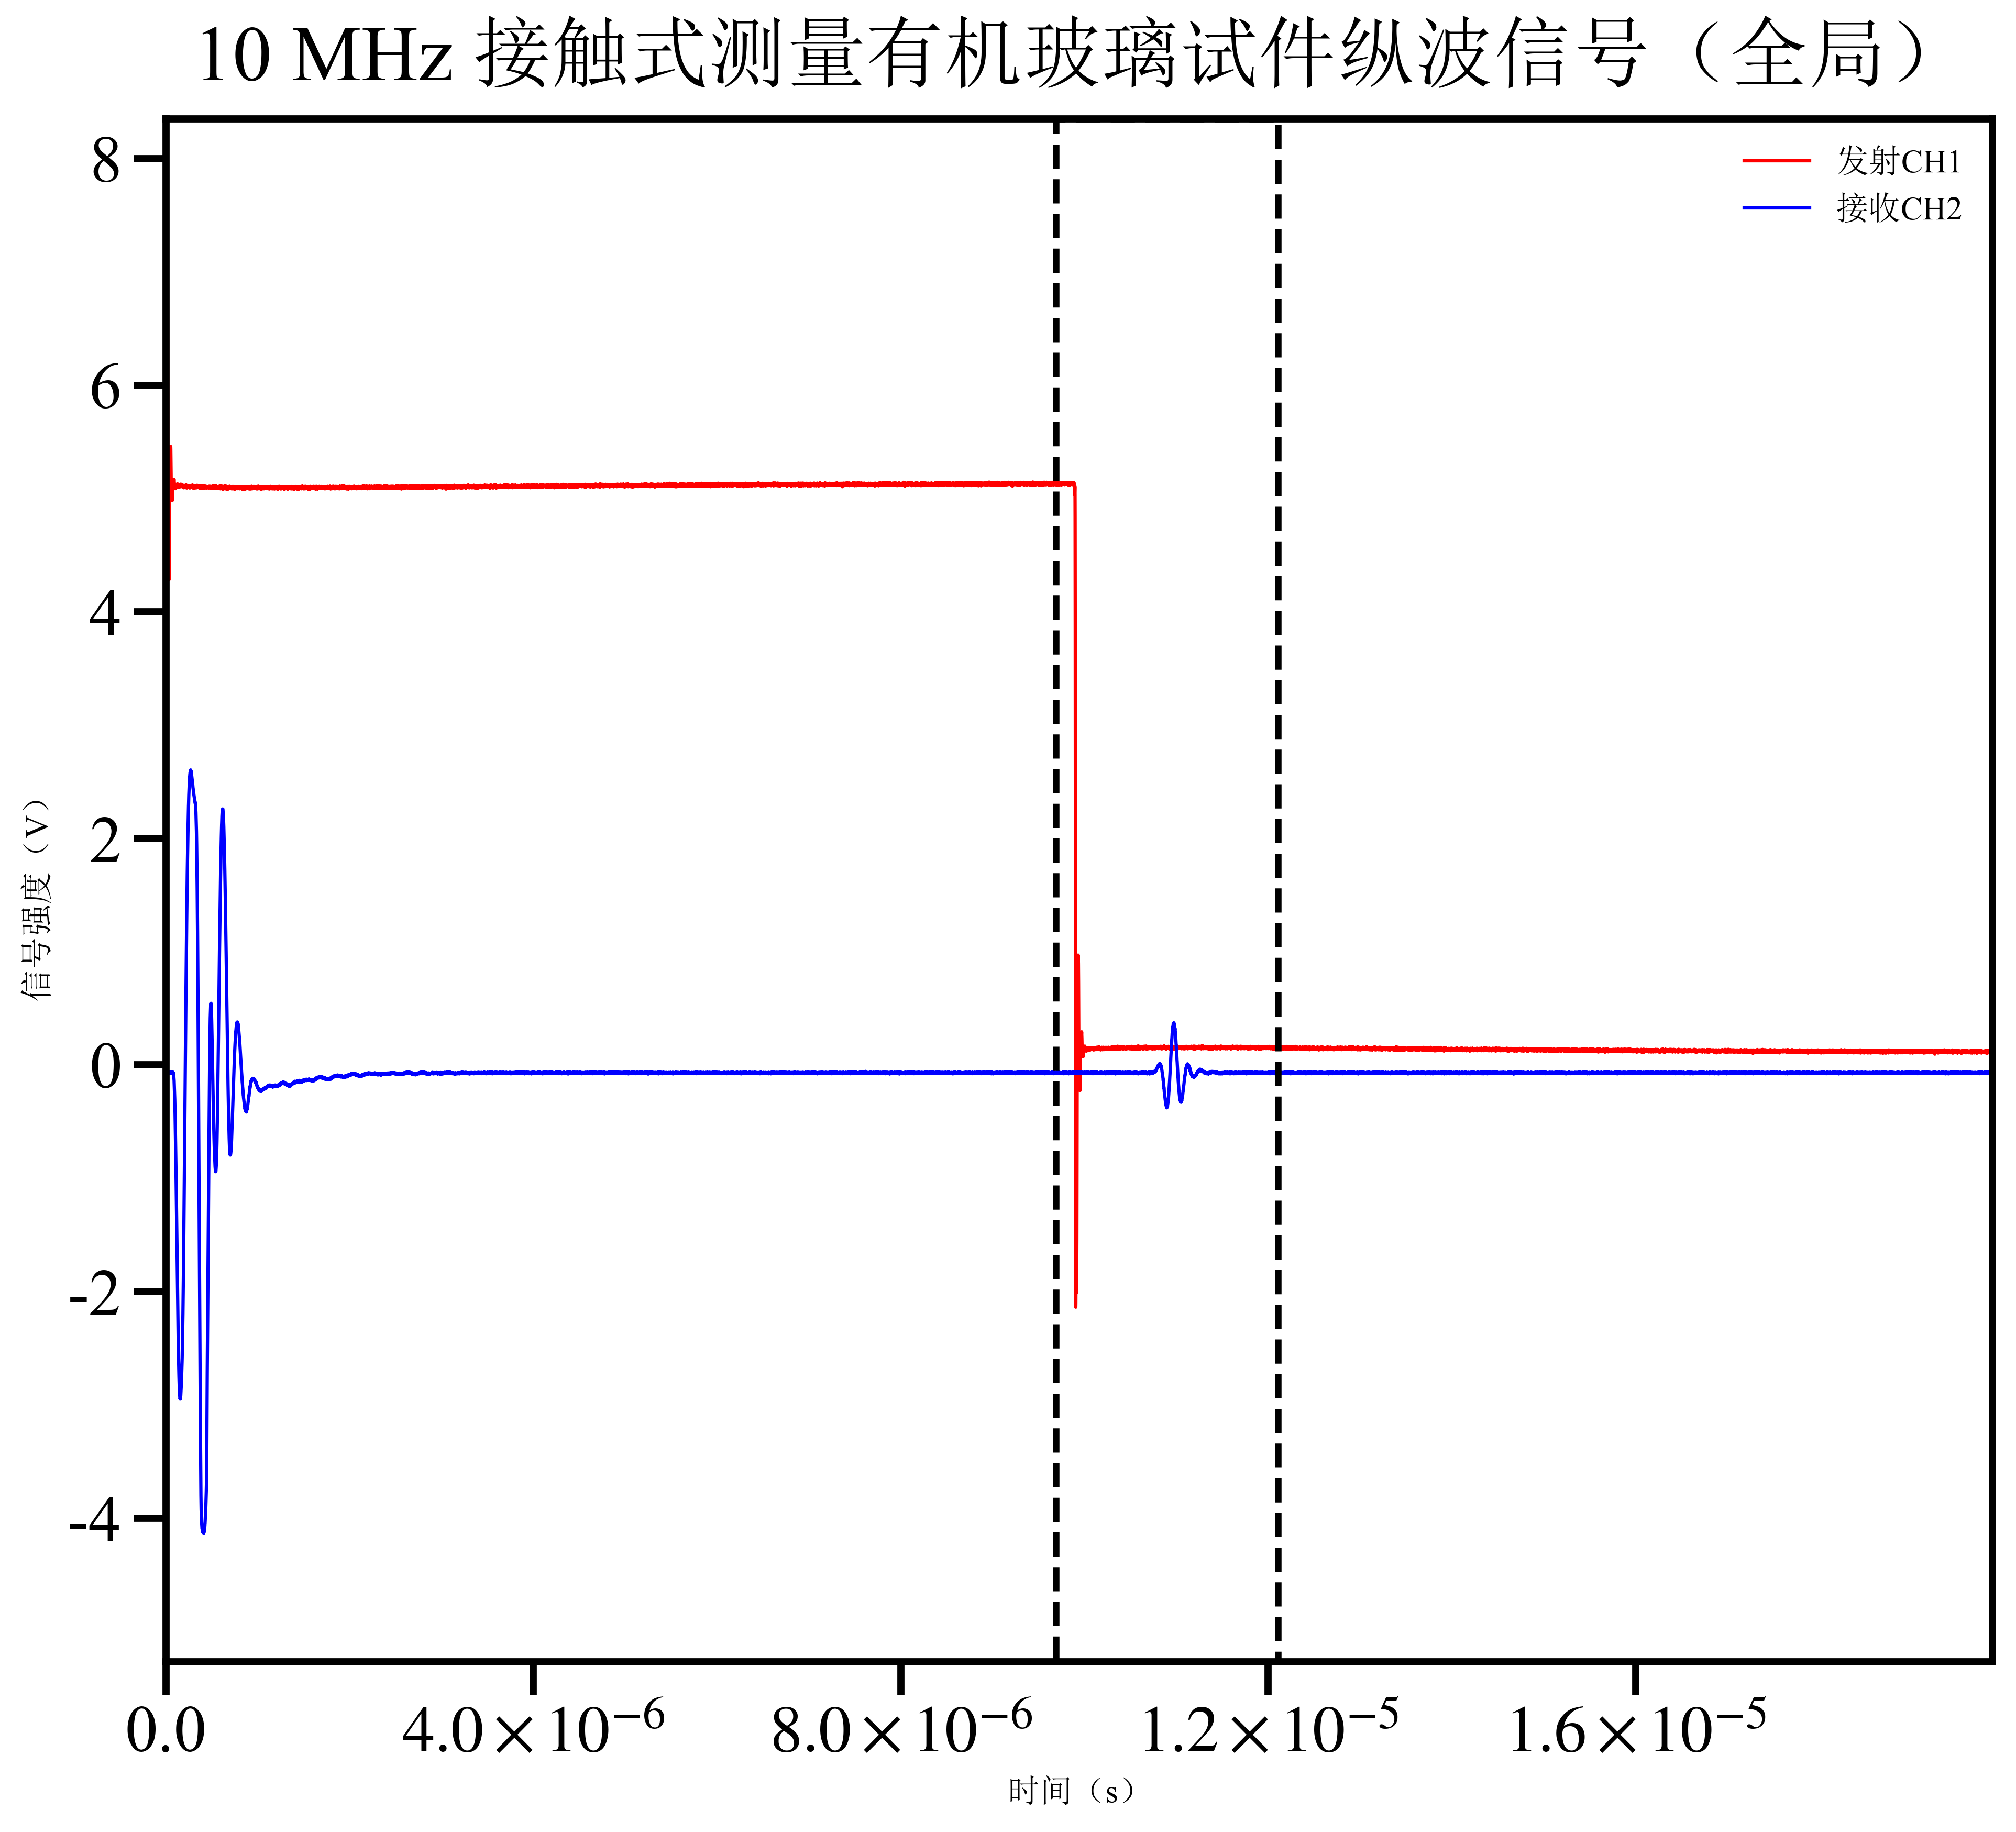
\includegraphics[width=\linewidth]{glass_10L_global.png}
  （a）输入输出信号全局图
\end{minipage}\hfill
\begin{minipage}[t]{0.48\textwidth}
  \centering
  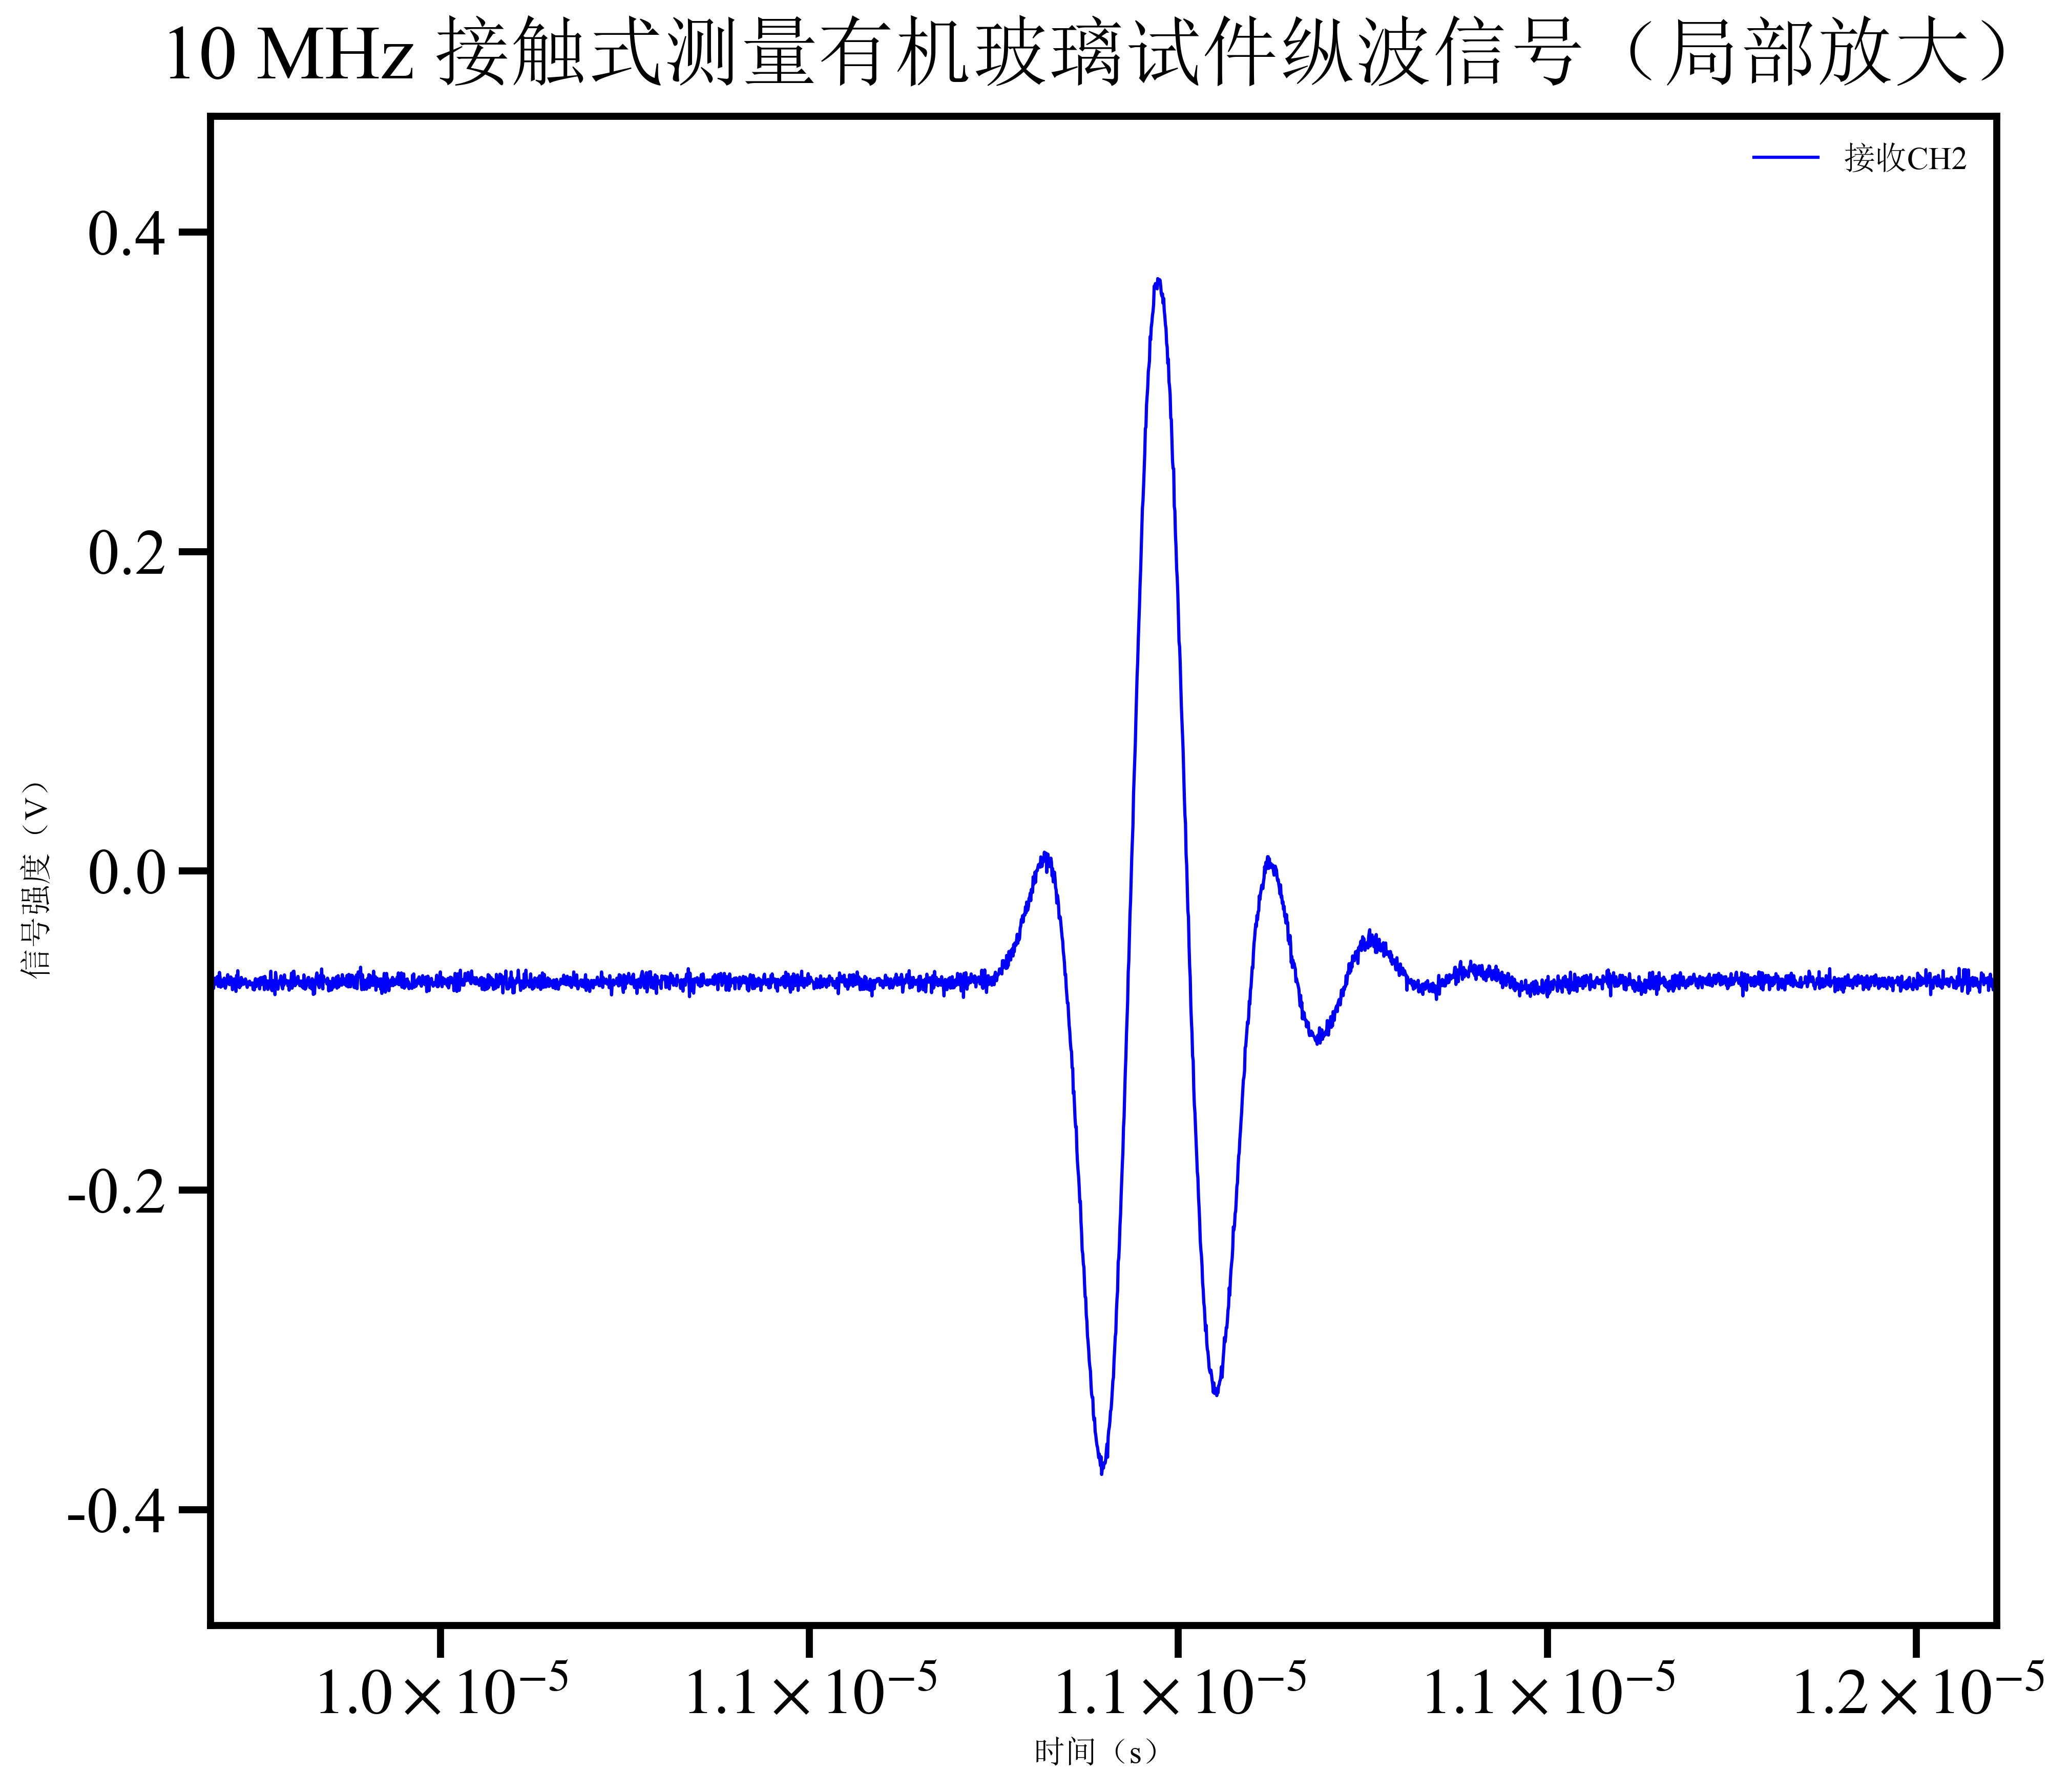
\includegraphics[width=\linewidth]{glass_10L_zoom.png}
  （b）输出信号局部放大图
\end{minipage}
\caption{10 MHz 接触式测量有机玻璃试件纵波波速时信号图}
\label{fig:exp2-og-10}
\end{figure}

\begin{table}[H]
\centering
\caption{5 MHz 与 10 MHz 接触式测量有机玻璃的纵波衰减系数}
\label{tab:exp2-frequency-attenuation}
\begin{tabular}{lccc}
\toprule
探头频率 & $P_m$（V），回波序号 $m$ & $P_n$（V），回波序号 $n$ & $\alpha_L$（dB/cm）\\
\midrule
5 MHz & 2.188，$m=1$ & 0.203，$n=2$ & 7.32\\
10 MHz & 0.378，$m=1$ & \multicolumn{2}{c}{仅检出单个回波，无法读取}\\
\bottomrule
\end{tabular}
\end{table}

将本结果与水浸法结果比较，讨论后续回波较弱、背景波、波峰选择和耦合剂均匀程度对衰减系数的影响。
有机玻璃 5 MHz 接触式测量的纵波衰减系数为 $7.32\,\mathrm{dB/cm}$，明显大于水浸法结果 $3.23\,\mathrm{dB/cm}$。接触式测量回波列短，第二回波幅值已降至 $0.203\,\mathrm{V}$，接近背景噪声，波峰选择对结果影响大；耦合剂层不均匀也会引入额外幅值起伏。10 MHz 信号仅检出单个回波，无法计算衰减系数，这与高频衰减更快的规律一致。

\section{采用脉冲回波法确定焊缝钢板中缺陷的位置及大小}
实验钢板尺寸为 $30\times30\,\mathrm{cm}^2$。首先在钢板表面绘制网格线，便于探头扫描点定位。在钢板表面涂抹适量纵波耦合剂，每次间隔 1 cm 进行 B-Scan；为提高精度，当扫描结果显示存在缺陷时改为每隔 0.5 cm 扫描一次并记录结果。

\subsection{钢板侧面垂直入射}
从钢板没有焊缝的侧面，采用 5 MHz 纵波探头进行探测。本组信号增益为 10 dB。当扫描路径上存在缺陷时，探头激励的超声波将提前被缺陷反射，在波形图中产生异常回波信号。记录缺陷反射主要出现的时间区间：$4\times10^{-5}\sim7\times10^{-5}\,\mathrm{s}$。在该区间取反射波形波峰和波谷对应信号强度绝对值中的最大值，作为该位置缺陷大小的度量，并绘制缺陷大小随位置变化的图线。

\begin{figure}[H]
  \centering
  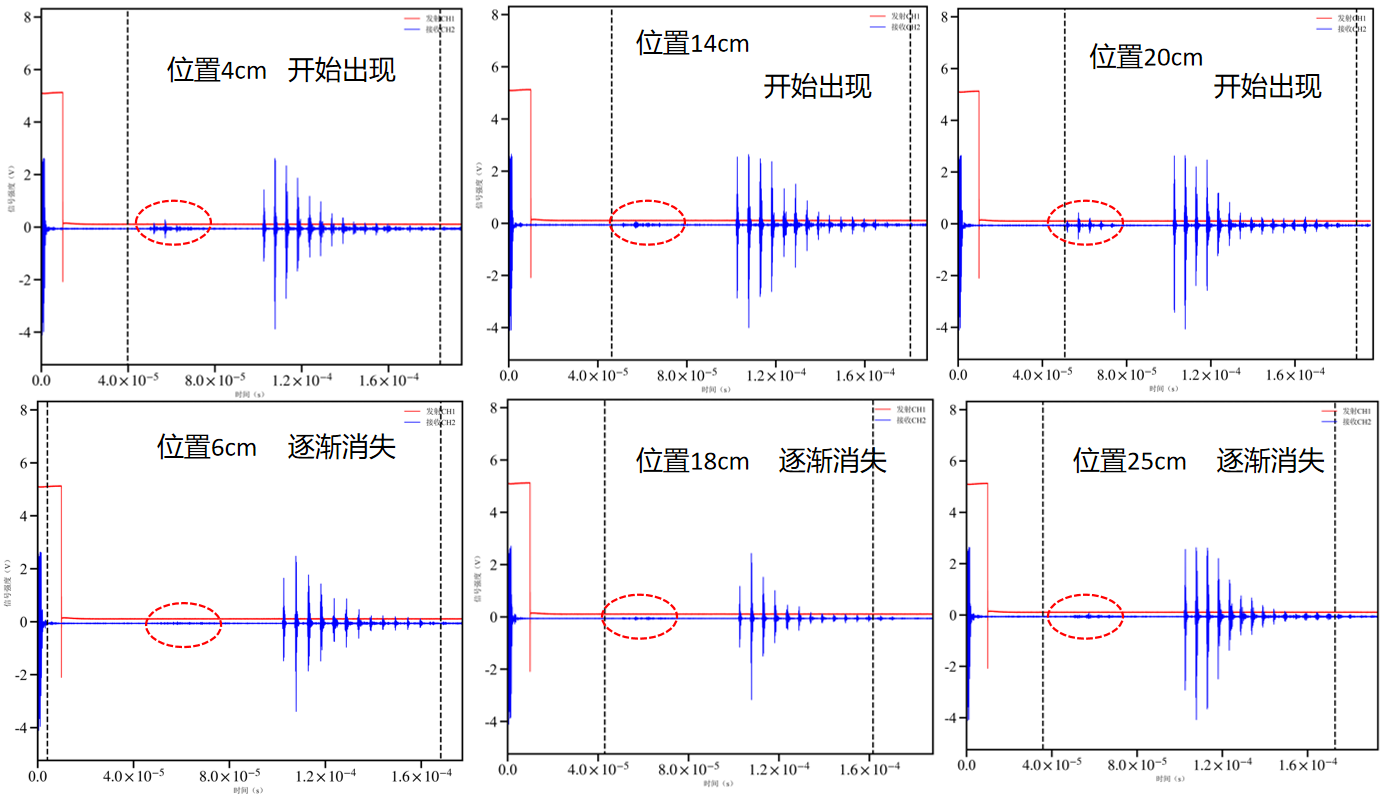
\includegraphics[width=16cm]{weld_L_summary.png}
  \caption{5 MHz 接触式纵波直探头测钢板焊缝：各位置缺陷反射信号}
\end{figure}
\noindent 缺陷位置与长度判断：缺陷信号在 4--6 cm、14--18 cm 及 20--25 cm 处出现。

\subsection{钢板表面斜入射}
在钢板有焊缝的表面采用 1 MHz 斜探头进行探测，本组信号增益为 30 dB，斜探头倾角为 $60^{\circ}$。记录缺陷反射主要出现的时间区间：$6\times10^{-5}\sim8\times10^{-5}\,\mathrm{s}$。按同样方法提取各位置缺陷反射强度并绘制损伤示意图。

\begin{figure}[H]
  \centering
  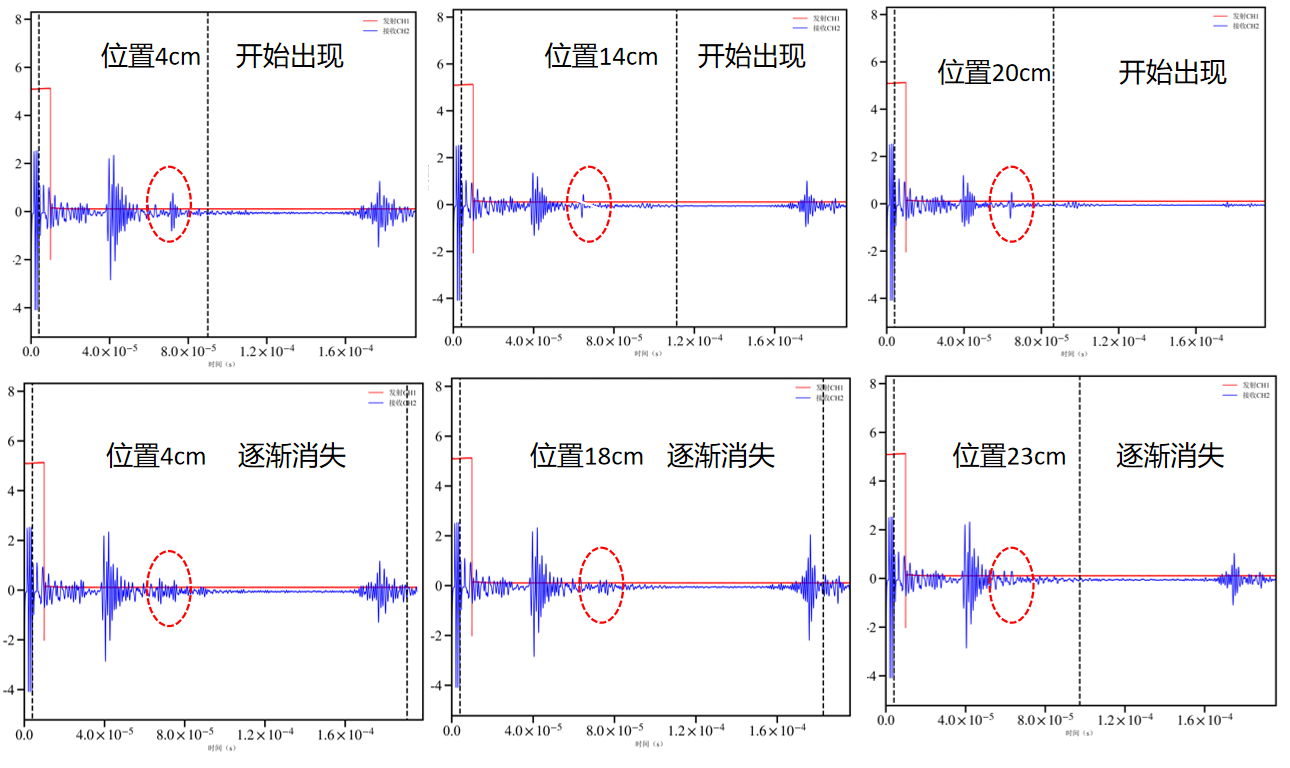
\includegraphics[width=16cm]{weld_S_summary.png}
  \caption{1 MHz 接触式斜探头测钢板焊缝：各位置缺陷反射信号}
\end{figure}
\noindent 缺陷位置与长度判断：缺陷在 4--6 cm、14--17 cm 及 20--23 cm 处出现。


\section{结果分析与讨论}
\begin{enumerate}
  \item 比较三种试件的纵波、横波波速及纵波衰减系数，并结合材料微观结构进行解释。声波在固体材料中传播时，其传播速度和能量传递效率与材料微观结构密切相关。金属材料如钢和铝在微观上主要由紧密排列的金属离子组成，周围有大量自由电子运动，这一结构赋予金属较高的密度和刚度。根据振动力学理论，较高的密度和刚度通常会提升声波传播速度并增强能量传递效率。相比之下，有机高分子材料由于分子间作用力较弱、密度较低、刚度较小，其分子链具有较强柔性，微观结构周期性弱，导致波在传播过程中发生更大的能量耗散，使其宏观表现出更低的波速和更大的衰减系数。
  \item 不同频率的超声探头各自具有优势与不足。频率较高的探头有利于发现更小的缺陷，且脉冲宽度小、分辨力高，有利于区分相邻缺陷；其波长短，半扩散角小，声束指向性好，能量集中，有利于发现缺陷并对缺陷定位。不利因素包括近场区长度大、随频率增加衰减急剧增加，并且对材料非均质性较敏感。因此，探头选择应根据具体实验需求，一般在保证检测灵敏度的前提下尽可能选用较低的频率。
  \item 在使用水浸法测量有机玻璃时，若波形图中出现较多非上下表面的回波，可分析探头是否做到完全垂直入射，以及部分波是否经过水面和底面反射造成噪音。
  \item 使用接触法测量金属试件时，若波形图中存在类似波包的结构，可考虑理想探测工况为无限大板，而实验室使用圆柱体，边界处可能发生波的反射甚至共振。
  \item 在缺陷探测中，两种探头在同一裂纹处所得的相对反射能量可能不同，因为两者对缺陷的探测角度不同。可根据这一点大致推断裂纹形状，并比较斜探头与直探头的测量结果。
\end{enumerate}
结合本组数据，补充结果分析与讨论。
本组数据中，钢、铝的纵波、横波波速与参考值偏差均在 $3\%$ 以内，且接触式与水浸式、5 MHz 与 10 MHz 的结果相互印证，说明测量系统稳定可靠。有机玻璃回波衰减快、杂波多，是误差的主要来源；其水浸信号中的杂波可能来自探头未完全垂直入射以及水面、盆底的反射。接触式测量金属圆柱试件时，回波列后可见较长的衰减尾，考虑为圆柱边界反射与共振所致。

\section{数据误差分析与提高精度的方法}
本实验每个量只记录一次，因此不计算由重复读数得到的标准差或 A 类不确定度。与参考值的相对误差仍可按前述公式计算。分析偏差时，应结合单次波形质量和实际操作判断，不能把一次读数的差异当作测量结果的离散性。
\begin{enumerate}
  \item 波速读数主要受试件厚度、探头位置和回波时间标记影响。接触式测量还应注意探头与试件是否贴合、耦合剂是否均匀；信号较弱时可合理调整增益，并保持读数规则一致。
  \item 衰减系数由同一波形的两个回波幅值计算。后续回波能量较低时，背景波和峰值选择对结果影响较大，应选取清楚、未重叠的回波，并记录所用的回波序号。
  \item 水浸法与接触法、5 MHz 与 10 MHz 探头属于不同测试条件，可比较其结果，但不能将这种差异当作同一条件下的重复测量误差。焊缝扫描中应保持探头方向和扫描间距一致。
\end{enumerate}
结合本组实际操作，补充主要偏差来源和可实施的改进措施。
本组主要偏差来源为：试件厚度等几何量均为单次读数，游标卡尺读数与测量垂直度直接影响波速基准；高衰减材料的后继回波接近噪声水平，波峰选取对衰减系数影响显著；接触式测量中探头贴合程度与耦合剂均匀性影响回波能量。可实施的改进措施包括：几何量多次测量取平均，固定波峰读取规则（统一取回波波包主峰），弱信号时适当提高增益并保持各次测量增益一致。

\end{document}
